\documentclass{tufte-book}

\usepackage{amsmath}
\usepackage{eurosym}
\usepackage[T1]{fontenc}
\usepackage[utf8]{inputenc}
\usepackage[estonian]{babel}
\usepackage[style=english]{csquotes}
\usepackage{nameref}

\hypersetup{colorlinks}% uncomment this line if you prefer colored hyperlinks (e.g., for onscreen viewing)

%%
% Book metadata
\title{Märkmeid \\infotehnoloogia\\ strateegiast}
\author[Andres Kütt]{Andres Kütt}
\publisher{Unpublished}

%%
% If they're installed, use Bergamo and Chantilly from www.fontsite.com.
% They're clones of Bembo and Gill Sans, respectively.
%\IfFileExists{bergamo.sty}{\usepackage[osf]{bergamo}}{}% Bembo
%\IfFileExists{chantill.sty}{\usepackage{chantill}}{}% Gill Sans

%\usepackage{microtype}

%%
% Just some sample text
%\usepackage{lipsum}

%%
% For nicely typeset tabular material
\usepackage{booktabs}

%%
% For graphics / images
\usepackage{graphicx}
\setkeys{Gin}{width=\linewidth,totalheight=\textheight,keepaspectratio}
\graphicspath{{graphics/}}

% The fancyvrb package lets us customize the formatting of verbatim
% environments.  We use a slightly smaller font.
\usepackage{fancyvrb}
\fvset{fontsize=\normalsize}

%%
% Prints argument within hanging parentheses (i.e., parentheses that take
% up no horizontal space).  Useful in tabular environments.
\newcommand{\hangp}[1]{\makebox[0pt][r]{(}#1\makebox[0pt][l]{)}}

%%
% Prints an asterisk that takes up no horizontal space.
% Useful in tabular environments.
\newcommand{\hangstar}{\makebox[0pt][l]{*}}

%%
% Prints a trailing space in a smart way.
\usepackage{xspace}

%%
% Some shortcuts for Tufte's book titles.  The lowercase commands will
% produce the initials of the book title in italics.  The all-caps commands
% will print out the full title of the book in italics.
\newcommand{\vdqi}{\textit{VDQI}\xspace}
\newcommand{\ei}{\textit{EI}\xspace}
\newcommand{\ve}{\textit{VE}\xspace}
\newcommand{\be}{\textit{BE}\xspace}
\newcommand{\VDQI}{\textit{The Visual Display of Quantitative Information}\xspace}
\newcommand{\EI}{\textit{Envisioning Information}\xspace}
\newcommand{\VE}{\textit{Visual Explanations}\xspace}
\newcommand{\BE}{\textit{Beautiful Evidence}\xspace}

\newcommand{\TL}{Tufte-\LaTeX\xspace}

% Prints the month name (e.g., January) and the year (e.g., 2008)
\newcommand{\monthyear}{%
  \ifcase\month\or Jaanuar\or Veebruar\or Märts\or Aprill\or Mai\or Juuni\or
  Julli\or August\or September\or Oktoober\or November\or
  Detsember\fi\space\number\year
}


% Prints an epigraph and speaker in sans serif, all-caps type.
\newcommand{\openepigraph}[2]{%
  %\sffamily\fontsize{14}{16}\selectfont
  \begin{fullwidth}
  \sffamily\large
  \begin{doublespace}
  \noindent\allcaps{#1}\\% epigraph
  \noindent\allcaps{#2}% author
  \end{doublespace}
  \end{fullwidth}
}

% Inserts a blank page
\newcommand{\blankpage}{\newpage\hbox{}\thispagestyle{empty}\newpage}

\usepackage{units}

% Typesets the font size, leading, and measure in the form of 10/12x26 pc.
\newcommand{\measure}[3]{#1/#2$\times$\unit[#3]{pc}}

% Macros for typesetting the documentation
\newcommand{\hlred}[1]{\textcolor{Maroon}{#1}}% prints in red
\newcommand{\hangleft}[1]{\makebox[0pt][r]{#1}}
\newcommand{\hairsp}{\hspace{1pt}}% hair space
\newcommand{\hquad}{\hskip0.5em\relax}% half quad space
\newcommand{\TODO}{\textcolor{red}{\bf TODO!}\xspace}
\newcommand{\na}{\quad--}% used in tables for N/A cells
\providecommand{\XeLaTeX}{X\lower.5ex\hbox{\kern-0.15em\reflectbox{E}}\kern-0.1em\LaTeX}
\newcommand{\tXeLaTeX}{\XeLaTeX\index{XeLaTeX@\protect\XeLaTeX}}
% \index{\texttt{\textbackslash xyz}@\hangleft{\texttt{\textbackslash}}\texttt{xyz}}
\newcommand{\tuftebs}{\symbol{'134}}% a backslash in tt type in OT1/T1
\newcommand{\doccmdnoindex}[2][]{\texttt{\tuftebs#2}}% command name -- adds backslash automatically (and doesn't add cmd to the index)
\newcommand{\doccmddef}[2][]{%
  \hlred{\texttt{\tuftebs#2}}\label{cmd:#2}%
  \ifthenelse{\isempty{#1}}%
    {% add the command to the index
      \index{#2 command@\protect\hangleft{\texttt{\tuftebs}}\texttt{#2}}% command name
    }%
    {% add the command and package to the index
      \index{#2 command@\protect\hangleft{\texttt{\tuftebs}}\texttt{#2} (\texttt{#1} package)}% command name
      \index{#1 package@\texttt{#1} package}\index{packages!#1@\texttt{#1}}% package name
    }%
}% command name -- adds backslash automatically
\newcommand{\doccmd}[2][]{%
  \texttt{\tuftebs#2}%
  \ifthenelse{\isempty{#1}}%
    {% add the command to the index
      \index{#2 command@\protect\hangleft{\texttt{\tuftebs}}\texttt{#2}}% command name
    }%
    {% add the command and package to the index
      \index{#2 command@\protect\hangleft{\texttt{\tuftebs}}\texttt{#2} (\texttt{#1} package)}% command name
      \index{#1 package@\texttt{#1} package}\index{packages!#1@\texttt{#1}}% package name
    }%
}% command name -- adds backslash automatically
\newcommand{\docopt}[1]{\ensuremath{\langle}\textrm{\textit{#1}}\ensuremath{\rangle}}% optional command argument
\newcommand{\docarg}[1]{\textrm{\textit{#1}}}% (required) command argument
\newenvironment{docspec}{\begin{quotation}\ttfamily\parskip0pt\parindent0pt\ignorespaces}{\end{quotation}}% command specification environment
\newcommand{\docenv}[1]{\texttt{#1}\index{#1 environment@\texttt{#1} environment}\index{environments!#1@\texttt{#1}}}% environment name
\newcommand{\docenvdef}[1]{\hlred{\texttt{#1}}\label{env:#1}\index{#1 environment@\texttt{#1} environment}\index{environments!#1@\texttt{#1}}}% environment name
\newcommand{\docpkg}[1]{\texttt{#1}\index{#1 package@\texttt{#1} package}\index{packages!#1@\texttt{#1}}}% package name
\newcommand{\doccls}[1]{\texttt{#1}}% document class name
\newcommand{\docclsopt}[1]{\texttt{#1}\index{#1 class option@\texttt{#1} class option}\index{class options!#1@\texttt{#1}}}% document class option name
\newcommand{\docclsoptdef}[1]{\hlred{\texttt{#1}}\label{clsopt:#1}\index{#1 class option@\texttt{#1} class option}\index{class options!#1@\texttt{#1}}}% document class option name defined
\newcommand{\docmsg}[2]{\bigskip\begin{fullwidth}\noindent\ttfamily#1\end{fullwidth}\medskip\par\noindent#2}
\newcommand{\docfilehook}[2]{\texttt{#1}\index{file hooks!#2}\index{#1@\texttt{#1}}}
\newcommand{\doccounter}[1]{\texttt{#1}\index{#1 counter@\texttt{#1} counter}}

% Generates the index
\usepackage{makeidx}
\makeindex

\begin{document}

% Front matter
\frontmatter

% r.1 blank page
\blankpage

% v.2 epigraphs
\newpage\thispagestyle{empty}
\openepigraph{%
Culture eats strategy for breakfast
}{Peter Drucker%, {\itshape Design, Form, and Chaos}
}
\vfill
\openepigraph{%
All warfare is based on deception
}{Sun Tzu}
\vfill
\openepigraph{%
\ldots all these must be built with due reference to durability, convenience and beauty
}{Marcus Vitruvius Pollio}


% r.3 full title page
\maketitle


% v.4 copyright page
\newpage
\begin{fullwidth}
~\vfill
\thispagestyle{empty}
\setlength{\parindent}{0pt}
\setlength{\parskip}{\baselineskip}
Copyright \copyright\ \the\year\ \thanklessauthor

%\par\smallcaps{Published by \thanklesspublisher}

\par\smallcaps{tufte-latex.github.io/tufte-latex/}

\par Litsents: Attribution-NonCommercial-ShareAlike 4.0 International, mis on saadaval \\ \url{http://creativecommons.org/licenses/by-nc-sa/4.0/}. \index{litsents}

\par\textit{Esmatrükk, \monthyear}
\end{fullwidth}

% r.5 contents
\tableofcontents

\listoffigures

%\listoftables

% r.7 dedication
\cleardoublepage
~\vfill
\begin{doublespace}
\noindent\fontsize{18}{22}\selectfont\itshape
\nohyphenation
Pühendatud ``patsiga poistele`` \\[5mm]Eriline tänu Priit Roosimägile ja Hanno Järvetile viidete, sisu ja tagasiside eest
\end{doublespace}
\vfill
\vfill


% r.9 introduction
\cleardoublepage
\chapter*{Sissejuhatus}

See dokument on kogum märkmeid ja bibliograafiat, mis on kogutud ette valmistades ja lugedes ainet IT Strateegiline juhtimine Tallinna Ülikoolis aastatel 2015 ja 2016. Sellisena ei moodusta ta tingimata tervikut vaid on oma olemuselt korvitäis mõtteid IT strateegiat puudutavatel teemadel.


\begin{figure*}[h]
	\begin{center}
		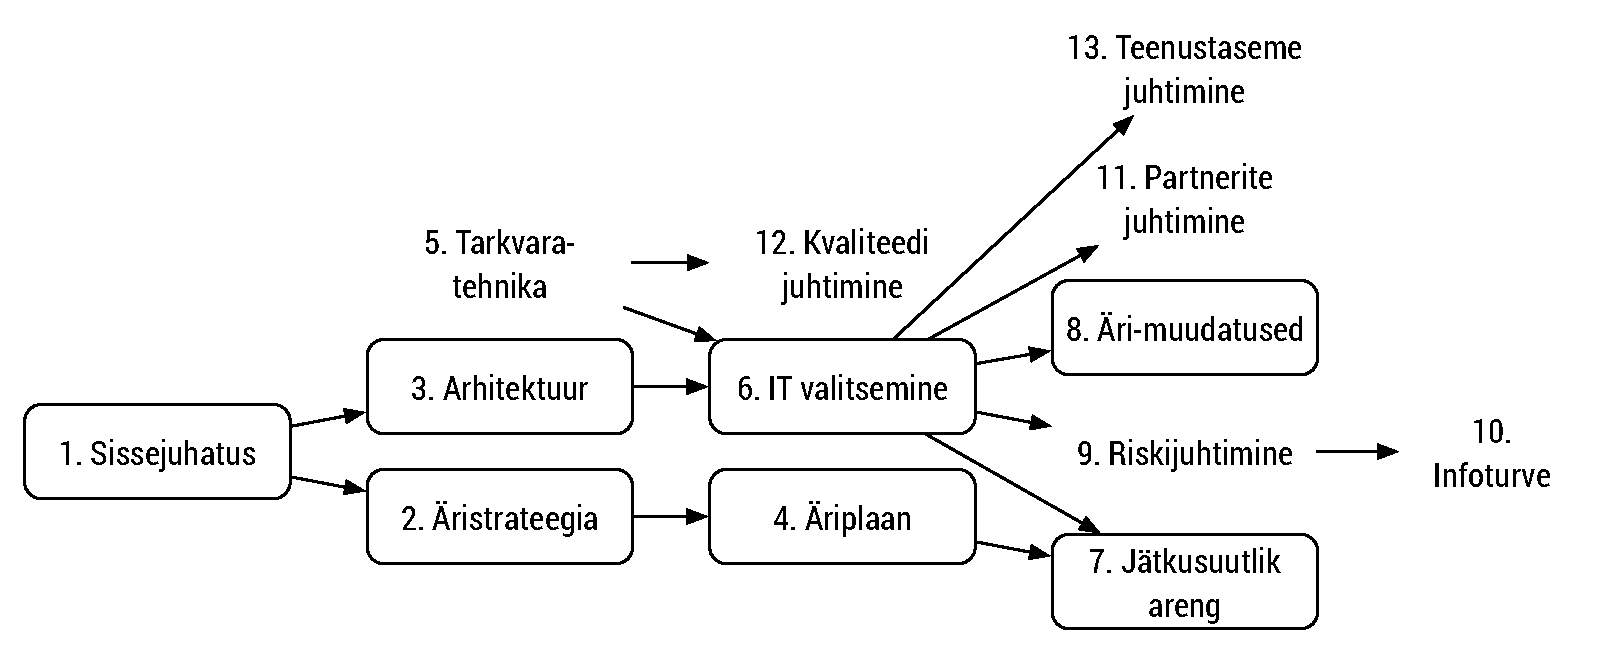
\includegraphics[width=\linewidth]{aine_struktuur.pdf}
		\caption{Teemade loogiline järgnevus ja seosed}
		\label{fig:intro:structure}
	\end{center}
\end{figure*}

Dokumendi struktuur tugineb loengute struktuurile, mis omakorda tugineb IT juhi kutsestandardile. Joonis \ref{fig:intro:structure} kujutab teemade ja peatükkide loogilisi seoseid (nooled) ja järjekorda (numbrid).

Iga peatüki lõpus on eraldi lõik aruteluküsimustega. Tegu ei ole mitte suurte lahendamatute probleemidega või isegi kõige kriitilisemate küsimustega. Need on probleemid, mille üle mõtlemine aitab usutavasti paremini mõttestada konkreetse peatüki sisu ning siduda seda IT juhi igapäevaeluga. Lisaks põgusale taustale iga küsimuse kohta sisaldab iga lõik nii autori mõtteid antud teemal kui ka loengus viibinud tudengite arutelu tulemusi.

%%
% Start the main matter (normal chapters)
\mainmatter

\chapter{Äristrateegia}
\section{Strateegia olemus}
Äritrateegiast on kõikvõimalikes vormides kirjutatud palju kuid siiski ei ole tegu valdkonnaga, kus eksisteeriks selgelt domineeriv mõttsuund. Ka strateegia enese definitsioon ei ole üheselt paigas ning seega onn paljul tavapäraselt strateegiaks peetul strateegia enesega vähe pistmist\cite{de2006strategy}. Freedman\index{Freedman, Lawrence} ütleb, et see peabki nii olema, sest ta strateegia tegeleb valikutega ning aruteluga nende üle. Valikud ise aga tuginevad laiale spektrile diskursustele.\cite{freedman2013strategy} 

Kuidas ka ei ole, \citeauthor{de2006strategy, rumelt1991strategic} toovad rea põhiküsimusi\cite{rumelt1991strategic}, millega äristrateegia selle ühel või teisel moel tegeleb:
\begin{description}\index{Strateegia!Põhiküsimused}
	\item[Eesmärgid] Mis suunas organisatsioon liigub ning, seeläbi ka vältimatult, mis suunas ta \emph{ei} liigu
	\item[Positsioon] Milline positsioon turul annab organisatsioonile suurima konkurentsieelise, olgu siis läbi olemasolevate resusrsside või turusituatsiooni. Turupositsiooni mõiste on samuti lai, kuid peamine on, et strateegia tegeleb organisatsiooni paigutamisega suhtes teiste turuosalistega. Näiteks on strateegiline küsimus, kas tegeleme pigem haljastusse või pensionäride tillukestesse aedadesse sobivate muruniidukitega.
	\item[Pakutavad tooted ja teenused] Millises sektoris organisatsioon osaleb ning milliseid teenuseid ja tooteid pakub. Kui eelmine küsimus oli seotud turuga, siis siin me saame näiteks küsida, kas me pigem tegeleme muruniidukite tootmise, hoolduse või näiteks laenutamisega
	\item[Tegevusulatus ja mitmekesisus] Kui suurt mitmekesisust pakutavates toodetes ja teenustes ning organisatsiooni tegevuses laiemalt talutakse ning kui suurt osa võimalikust toodete/teenuste spektrist kaetakse
	\item[Ressursside suunamine] Kuhu me kulutame oma piiratud ressursid. Tegemist on teatud mõttes juhtimisliku põhiküsimusega keerulise komplekti piiratud vahendite kulutamisest võimalikult kasulikul moel. Kuigi strateegia ei saa anda siin täpset vastust, peab ta vastuse leidmist toetama. Strateegia ei ütle, mitu inimest tegeleb müügi ja mitu klienditeenindusega kuid ta võib öelda, et meie jaoks on müük olulisim ning klienditeenindus pole oluline
	\item[Organisatsiooni disain] Milline on organisatsiooni struktuur, millised poliitikad kehtivad ning milliseid administratiivseid vahendeid kasutatakse. Ehk, kuidas organisatsioon määratleb ja koordineerib tööd
\end{description}


Siinkohal võib tekkida küsimus, kus nende küsimustega igapäevane tegelemine muutub taktikast strateegiaks. Freedman ütleb, et tegelikult on vahe strateegia ja taktika vahel seotud vaid organisatsiooni hierarhia ning vähemal määral otsuste mõju ning ajahorisondiga. Kuid mõlemal juhul on otsuste taga samad printsiibid. 
\begin{marginfigure}
	\begin{center}
		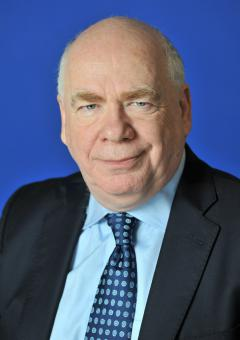
\includegraphics[width=.84\linewidth]{freedman.jpg}
		\caption{Lawrence Freedman}
		\label{fig:freedman}
	\end{center}
\end{marginfigure}

Üsna levinud on kontseptsioon \enquote{strateegilisest plaanist}\index{Strateegia!Plaan}. Ehk arusaam, et strateegia seab eesmärgid ning sammud nendeni jõudmiseks. Nii mõtlevad tihti insenerid: meil on lahendamist vajav probleem, me töötame välja plaani ja viime selle ellu. Meil on vaja kuule jõuda ning sinna me ka jõuame. Konks on selles, et kuu ei ürita raketi ehitamise käigus aktiivselt eest ära joosta. Nii arutledes on raske mitte nõustuda Freedmaniga, kes ei pea õigeks mõelda strateegiast kui plaanist\sidenote{Ta tsiteerib Mike Tysonit\index{Tyson, Mike}: \enquote{Everyone has a plan 'till they they get punched in the mouth}}. Tema argumentatsioonis tugineb strateegia alati organisatsiooni positsioonile ning positsiooni muutudes muutub ka strateegia, eesmärgid ja plaan. Strateegia praktiline iva ei ole Freedmani järgi mitte mingi konkreetse eesmärgi saavutamine vaid jõudmine praegusest paremasse positsiooni. Samuti ei lõpe miski eesmärkide saavutamisega. Revolutsioonile järgneb vajadus valitseda, konkurendi üle võtmisele vajadus ühist organisatsiooni ehitada\sidenote{\enquote{Strategy is not a three-act play. It's a soap opera}}. 


Milline siis on Freedmani konstruktiivne vaade strateegiale? Tema käsitluses on strateegia aluseks soov kontrollida tulevikku suuremal määral, kui konkurendid. Tuleviku ennustamise aluseks on aga mõttemudel. Mõttemudeli mõistet seletab ehk kõige paremini Hawking\cite{mlodinow2010grand}. Ta väidab, et me tajume maailma alati läbi mudeli ning et selle mudeli peamiseks omaduseks on tema ennustusväärtus: kui täpselt suudab mudel mineviku alusel ennustada tulevikku. \sidenote{Hea mõttemudel ei ole siiski tingimata seotud isikliku heaoluga. Giordano Bruno mudel oli valitsevast maailmakäsitlusest oluliselt parema ennustusväärtusega}. 

Seega muutub strateegias põhimõtteliseks küsimuseks sobiliku mõttemudeli loomine, praeguse olukorra mõtestamine organisatsiooni soovitud suunas liigutada aitaval viisil. Kuid organisatsioon ei koosne ainult juhist ning seega on strateegia puhul oluline, et organisatsiooni liikmed võtaksid omaks just juhi loodud malli ning suudaksid ja tahaksid seda ka tegutesse valada. See on juhi töö, mille aluseks on teatud empaatiavõime. Ei ole mõeldav asendada üht mõttemudelit teisega toda esimest esmalt mõistmata. Üheks viisiks tagada mõttemudeli jagatust on kaasata organisatsioon selle koostamisse. Tuleb nõustuda Eisenhoweriga\index{Eisenhower, Dwight D.}, kes ütles \quote{\enquote{Plans are worthless, but planning is everything}}. 

Kuigi strateegiat ei ole mõistlik vaadata liikumisega konkreetse eesmärgi poole, on strateegia kui teema mõistmiseks oluline mõista organisatsioonide liikumapanevaid jõude. \citeauthor{de2006strategy} sõnastab selle nii:

\begin{center}
	\textbf{Väärtuse loomine omanikele ning teistele osapooltele läbi kliendile väärtuse pakkumise}
\end{center}

On oluline mõista, et \enquote{väärtus}\index{Väärtus} võib tähendada oluliselt laiemat mõistete skaalat, kui lihtsalt finantstulu. Väärtust reeglina \emph{mõõdetakse} rahas kuid ta ei pruugi \emph{olla} rahaline. Nii mõnigi pillimees peab muusikastuudiot mitte sellest omanikutulu teenimiseks kui omamaks võimalust igal hetkel koos sõpradega oma hobiga tegeleda. Ehk, väärtus on oma olemuselt subjektiivne. 

Siit näeme, et organisatsiooni liikumissuund on sõltuv omanikest ning \enquote{teistest osapooltest}. Kui omaniku mõiste on reeglina juriidiliselt täpselt määratletud, siis teiste osapoolte määratlus on segasem\sidenote{Ja, globaalses kontekstis, järjest segasemaks läheb. Vt. \nameref{sec:architecture:paradigm}}. 

Oleme näinud, et strateegia on oma olemuselt dünaamiline nähtus. Teda suunavad vähemalt kolm võtmefaktorit:
\begin{itemize}
	\item Strateegia ise läbi organisatsiooni positsiooni ning seega ka strateegia nihutamise
	\item Organisatisooni omanike\index{Omanik} ja arvesse võetavate \enquote{teiste osapoolte} ringi muutused
	\item Omanike ja teiste osapoolte arusaam väärtusest\sidenote{Eriti keeruline strateegiline olukord tekib, kui omanike ja muude huvigruppide arusaam väärtusest aeglaselt lahku triivivad}
\end{itemize}
\begin{marginfigure}
	\begin{center}
		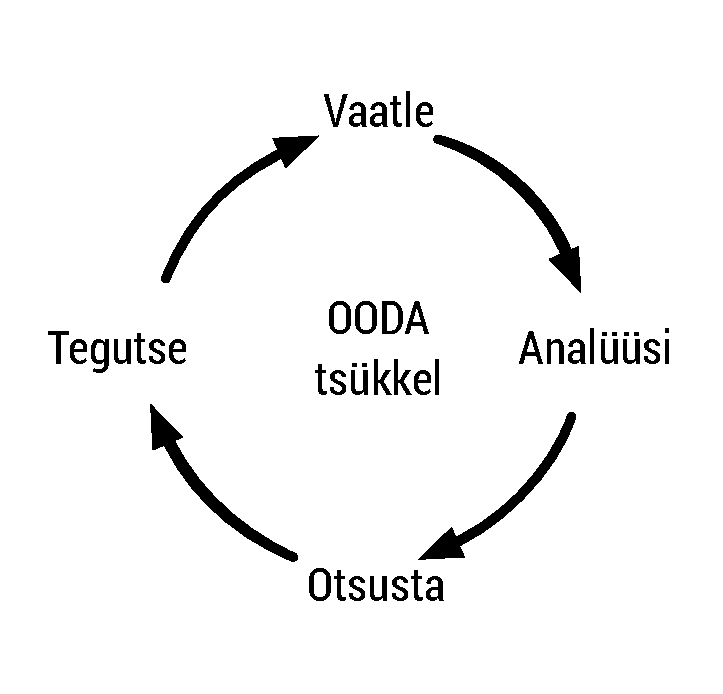
\includegraphics[width=\linewidth]{ooda.pdf}
		\caption{OODA/VAOT tsükkel}
		\label{fig:ooda}
	\end{center}
\end{marginfigure}

Strateegiast kui dünaamilisest nähtusest aitab ehk mõelda VAOT\sidenote{Originaalis \emph{OODA. Observation, Orientation, Decision, Action}} tsükkel, mille autoriks on John Boyd\index{Boyd, John}. Boyd oli inseneritaustaga lendur ja militaarteoreetik kelle karjäärist paistab harvanähtav võimekus tegeleda probleemidega väga laial abstraktsiooniastmete skaalal. Oma kogemusest lahinglendurina suutis ta sünteesida mõjukaid teooriaid, neid populariseerida ning suunata ka nende  rakendamist. Tema VAOT tsükkel koosneb järgmistest, järjest korduvatest, sammudest:

\begin{description}
	\item[Vaatle] Kogu andmeid olukorra kohta
	\item[Analüüsi] Analüüsi ja sünteesi kogutud andmeid lähtudes oma hetkepositsioonist ja mõttemudelist
	\item[Otsusta] Määra, jällegi tuginedes oma mõttemudelile, kindlaks tegutsemissuund
	\item[Tegutse] Vii otsused ellu
\end{description}


Boyd'i idee seisnes selles, et võitmiseks\sidenote{Freedman osundab, et võit on strateegilises mõtlemises liigselt rõhutatud. Tõpeoolest, Napoleoni strateegia tugines suuresti otsustavale võidule kuid ka tema 1812. aasta sõjakäik näitas, et see ei ole alati võimalik. Tänapäevases tehnoloogiliselt keerulises olukorras on nii militaarselt kui äriliselt üha raskem vastast otsustava löögiga põlvili sundida. Strateegia oluliseks komponendiks on võimekus oodata, koalitsioone moodustada ja mitte kohe rünnata.} tuleb luua olukordi, kus ollakse suuteline vastasest kiiremini õigeid otsuseid tegema. Nii ei ole teisel osapoolel võimalik õigesti käituda: olukord muutub enne, kui te reageerida jõuab. Sellest ka keskendumine otsustusprotsessile ning adapteerumisele mitte ühele konkreetsele olukorrale vaid muutuvale situatsioonile üldiselt.

\section{Strateegiamõtte ajaloost}
Strateegia mõiste sellisena, nagu me teda täna tunneme, kerkis esile militaarvaldkonnas 18. sajandil. Sõna \emph{stratagos} tähendabki kreeka keeles kindralit ja seega on strateegia läbi ajaloo olnud seotud just militaarvaldkonnaga.

\index{Sõjakunst}Siiani on kasutatav näiteks klassikaline\sidenote{Tegu on sel määral klassikalise teosega, et ka selle kommentaarid on juba klassika. Ongi mõistlik hankida kõige põhjalikuma võimaliku kommentaariumiga väljalase, kommentaarid koondavad strateegiamõtte väga paljude sajandite jooksul} sõjakunsti õpik The Art of War\cite{tzu2013art}. Seal määratleb autor muu hulgas viis võidu peamist osist. Nende otsene rakendatavus tänapäeval on heaks näiteks vanameistri mõttesügavusest. Tema järgi võidab see, kes

\begin{description}
	\item[Kes teab, millal võidelda ja millal mitte] Inglise keeles on kena ütlemine \emph{\enquote{pick your fights}} ja seda siin mõeldaksegi. Hea strateeg otsustab oma võitluste üle teadlikult ning oskab sedalaadi otsuseid teha.
	\item[Kes teab, kuidas toimida tugevama ja nõrgema vastasega] Strateegia peab sõltuma kontekstist ja konkurentidest. Tugevama vastasega jõudu katsuma minna ei ole nutikas ning nõrgema vastase hävitamine tekitab vaid probleeme.
	\item[Kelle armee kõik astmed on täidetud samast vaimust] Siin kehastub Peter Druckeri\index{Drucker, Peter} ütlus \emph{\enquote{Culture eats strategy for breakfast}}\index{Kultuur}\sidenote{Seda kuulsat tsitaati ei leia ühestki Druckeri kirjutisest. Ütluse omistas talle esmakordselt Mark Fields\index{Fields, Mark} Fordist 2006. aastal ning, väidetavasti, ripub see siiani Ford Motor Company \emph{war room}i seinal}. Mõte on selge: ilma jagatud väärtuste, tõekspidamiste ja uskumusteta on väga keeruline organisatsiooni ühtsena toimima panna
	\item[Kes, olles ise valmis, ootab, tabamaks vastane ootamatult] Ühest küljest korratakse siin esimest mõtet kontrollist olukorra üle kuid teisalt tuuakse sisse ka vastasele ootamatu käitumine ning seega ka eristumine\sidenote{Vt. pikemat arutelu eristumisest lõigus \nameref{sec:governance:bp}}
	\item[Kellel on suveräänist segamata sõjaline võimekus] Seda strateegia aspekti käsitletakse teistest suhteliselt harvem kuid tegu on kindlasti olulise strateegilise eelisega. Strateegiliseks manööverdamiseks vajab juht vabadust otsustada, alluvate respekti ning teadmist, et teda usaldatakse. Kõike seda Sun Tzu ka ütleb. 
\end{description}

Sun Tzu kriitikud, sealhulgas Freedman\index{Freedman, Lawrence}, väidavad, et tema \enquote{ole nutikam kui teised} lähenemine ei ole tingimata korratav ega eelist andev. Jõult nõrgema vastase kaval nõks võib läbi minna kuid ei pruugi. Ning kui kõik üritavad üksteist üle kavaldada, on tulemuseks patiseis. Siiski on Sõjakunstis kindlasti väärtuseks suund otsese vägivaldse konflikti vältimisele ka siis, kui ollakse ülekaalus.

Juhtimisse jõudis strateegia alles eelmise sajandi kuuekümnendatel surevestatuna suuresti korporatsioonide jõudmisest ekspansiivse kasvu piirideni. Kuna seadused hakkasin piirama edasist ühinemist ja turu haaramist, tuli keskenduda kasumlikkusele. Seega on varane strateegiamõte suuresti suunatud organisatsioonide sisse\sidenote{Ehk, ta on olemuselt sarnane IT juhi väljakutsetega, kes samuti tegeleb olemasolevast maksimumi võtmisega.} ja ei tegele eriti konkurentsiga. 

Strateegia kui valdkonna arengust seitsmekümnendatel ja kaheksakümnendatel (ning suurepärase nimekirja klassikalistest artiklitest) annab \citeauthor{rumelt1991strategic} essee\cite{rumelt1991strategic} .

\section{Hea ja halb strateegia}
\label{sec:strategy:goodbad}

\begin{marginfigure}
	\begin{center}
		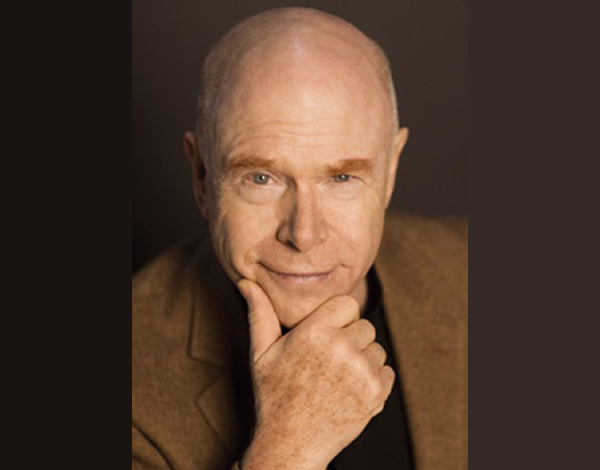
\includegraphics[trim={5cm 0 5cm 0},clip,width=.7\linewidth]{richard_rumelt.jpg}
		\caption{Richard Rumelt}
		\label{fig:rumelt}
	\end{center}
\end{marginfigure}

Üks põnevamaid tänapäevaseid arhitektuurimõtlejaid on Richard Rumelt\index{Rumelt, Richard}. Tema taust on inseneerias, seitsmekümnendatel osales ta kosmosesondi Voyager 1 konstrueerimisel. Tema ehk kuulsaim teos \enquote{Good strategy/bad strategy}\cite{rumelt2011good}. Raamatu allikaks on frustratsioon kuristikust srateegia ning tavaliselt strateegiaks nimetatu vahel\sidenote{Hea ülevaate tema seisukohtadest annab \url{https://www.youtube.com/watch?v=UZrTl16hZdk}}. Kui Steve Jobs\index{Jobs, Steve} 1997. aastal uuesti Apple juhiks sai, ei usutud tema edusse. Ometi suutis ta organisatsiooni mitte ainult päästa vaid ka ümber pöörata tehes asju, mida õpitakse ülikoolis esimesel kursusel. Ta loobus kõigest mittevajalikust keskendudes Apple äri tuumale. Rumelt ütleb, et keegi tegelikult ei oota, et keegi päriselt sel viisil strateegiaga tegeleb. Ehk, hea ja koherentne strateegia on haruldane ning üllatav.

Eespool kirjeldatud vaade strateegiale sisaldas sõnu nagu \enquote{turg} ja \enquote{konkurents} kehastades seega probleemi ökonomeetrilist aspekti. Kuigi kahtlemata õige, ei ole selline lähenemine kergesti rakendatav vabakonna, avaliku sektori ja näiteks koolide puhul ehk olukordades, kus turust ja teenustest rääkimine on keeruline\sidenote{Vt. pikemat arutelu \cite{rumelt1991strategic}}. Siia kuuluvad ka IT organisatisoonid, kes küll opereerivad ärilises keskkonnas kuid kelle tegevuse mõõdikud on harva puhtalt majanduslikud.

Rumelt pakubki alternatiivi sõnastades mitte strateegia definitsiooni vaid \enquote{hea} ja \enquote{halva} strateegia tunnused. 

Tema järgi on halb strateegia\index{Strateegia!Hea ja halb} selline:
\begin{description}
	\item[Keskendub eesmärkidele] Strateegia on tihti kombinatsioon toredatest asjadest ja asjadest, mida me tahaksime saavutada. Eesmärkide sõnastamine on kahtlemata oluline aga strateegia peaks ütlema ka midagi nende saavutamise kohta. Kui meie straeegia on \enquote{20\% kasumimarginaali ja 20\% käibekasvu aastas}, siis mida me siis ikkagi selle saavutamiseks teeme?
	\item[On pehme ja kohev] Selline strateegia on ebamäärane kasutades raskesti defineeritavaid mõisteid ja ebaselgeid kontseptsioone. \enquote{Oleme kliendikeskne innovatsiooniliider läbi tarneahela sünergia võimendamise} kõlab uhkesti aga strateegia ei saa olla otsuste aluseks ilma, et ta oleks üheselt ja selgelt arusaadav. 
	\item[Ei sisalda probleemi] Räägitakse asjadest, mida me loodame saada, rääkimata olukorrast, kus me oleme. Et kuhugi minema hakata, on oluline kokku leppida, kus parasjagu ollakse ja kuidas seda olukorda mõttestatakse. On oluline vahe, kas organisatsioon on \emph{ainult} või \emph{juba} kaheksakümneprotsendiline turuosa
	\item[Sarnaneb Tootsi peenrale] Selline strateegia sisaldab hirmpikka loetelu eri asjadest, millega organisatsioon peaks tegelema ning mida kõike saavutama. Paraku on suur osa olulisi eesmärke üksteist välistavad ning nii ei ütle selline strateegia midagi peale selle, et selle koostaja ei suuda valikuid teha
\end{description}

Hea strateegia tunnused pakub Rumelt välja järgmised:
\begin{description}
	\item[Tal on selge kolmeosaline tuum] Hea strateegia peab sisaldama diagnoosi (kuidas me mõttestame meie ees seisva probleemi\sidenote{Huvitaval kombel teeb Rumelt eelduse, et kõigil on probleemid. Et kõigil on keskne hulk jõude, milledele vastu seismine nõuab pingutust. On üsna keeruline ette kujutada, millised on need jõud näiteks Apple või Google puhul. Kahtlemata on neil väljakutseid kuid tõenäoliselt on raske välja tuua üht ja eksistentsiaalset.} tuuma), juhtpoliitikat (milles meie lahendus seisneb) ja koherentset tegevusplaani (millised sammud võetakse ette probleemi lahendamiseks)
	\item[Sisaldab saavutatavat eesmärki] Hea strateegia osa on miski, mida on võimalik teatud pingutusega usutavalt saavutada. See miski peab olema konkreetne ning suhteliselt lühikese ajahorisondiga. Selline eesmärk annab tegevusele suuna ning aitab hinnata progressi
	\item[Eeldab entroopiat ja inertsi] \index{Entroopia}Strateegia rakendamise puhul on kõige suuremaks raskuseks tõenäoliselt organisatsioon ise. Algne plaan muutub ajas ja organisatsiooni hierarhias liikudes järjest hägusamaks ja sellega tuleb arvestada. Samuti on alust eeldada, et muutused organisatsioonis vastuseisu tekitavad ning plaan peab seda peegeldama
\end{description}

\section{Strateegia kasutusest}
\label{sec:strateegia:kasutu}
Oma strateegia ajaloos osundab Freedman, et Lääne kultuuriruumis kerkis strateegia kui oluline kontseptsioon esile alles kaheksateistkümnendal sajandil seoses sõja kui sellise keerukuse kasvuga\cite{freedman2013strategy}. Ühest küljest tekkis arvamus, et sõda, nagu teisedki eluvaldkonnad võiks süsteemsest mõtlemisest kasu saada. Kuid teisalt muutus sõda oma massiarmeede ja logistika-ahelatega ühte peasse mahtumiseks liiga keeruliseks. Enam ei olnud võimalik strateegia formuleerimist ja ellu viimist mõistlikult ühendada. Ka äristrateegia esile kerkimist seostab ta ettevõtete praktilise vajadusega liikuda kvantitatiivselt kasvult kvalitatiivsele.

See, loomulikult, ei tähenda, et varasemalt kuidagi oskamatult sõditud või firmasid juhitud oleks. Puudus lihtsalt praktiline vajadus eraldiseisva strateegia kontseptsiooni järele. Piisas kas lihtsast õnnest või usust geniaalsesse sõjapealikkusse. Strateegia oli suuresti välja hääldamata ning juurtega kommetes ning tavades\sidenote{Keeley war before civilization via Freedman}

Siit tuleneb oluline järeldus: strateegiat ei ole alati vaja. Kuna töö on ressursi- ja ajamahukas (ning kasutu strateegia taustal võib kergesti rumalasse olukorda jääda), siis on oluline mõista, millal strateegiaga tegeleda ei ole mõtet.

Skype\index{Skype} varastel aastatel puudus ettevõttel strateegiadokument selle klassikalises mõttes. Ei toimunud ka eraldi strateegia arendamise protsessi. Ometi võis juhusliku kontoris kohatud inimese käest saada küsimusele \enquote{millega te siin tegeleme?} konkreetse ja ammendava vastuse. Ja need vastused langesid põhijoontes kokku. Kuidas nii? Meie ees toona seisnud probleem oli väga konkreetne ja üheselt arusaadav ka ilma suuri sõnu tegemata. Oli vaja ise ellu jäädes telekomiturg pikali lükata. Suhteliselt väikeses kitsa ringi inimeste ümber koondunud organisatsioonis on tegemist vajav selge ka ilma eksplitsiidse strateegiata. 

Piibel ütleb, et \enquote{võidujooks pole kiiretele ja lahing tugevatele}. Ja, tõesti, suure hulga ressursside igasugune enam-vähem mõistlik kasutamine viib reeglina soovitud tulemusele ka ilma suurema strateegiata. Võib kuluda vähem või rohkem aega või ressursse aga töö saab tehtud. Nagu insenerid vahel ütlevad: \enquote{Ei ole lahendamatuid probleeme, on liiga väikesed haamrid}. Kui paras haamer käepärast ei ole mõtet arutada, kas võtta ta paremasse või vasakusse kätte.

Kolmas põhjus strateegiat mitte omada on kontrolli puudumine. Isegi kui käsitleda strateegiat kui suure hulga isiklike strateegiate sünergeetilist summat, on strateegia kujundamiseks ikkagai vaja neid isiklikke lähenemisi suunata. Kontroll võib puududa kas ülemiste juhtimistasandite poolt seatud reeglite, alumiste tasandite vastuseisu või usalduskreedidi puudumise tõttu juhi vastu. Kuidas ka ei oleks, sellisel juhul strateegiaga tegelemine on kindel viis end lolliks teha. 

Kokkuvõttes, strateegiaga ei ole mõtet tegeleda kolmel juhul:
\begin{itemize}
	\item Kui ollakse väike ning keskendunud
	\item Kui ollakse suur ja tugev
	\item Kui olukorda ei kontrollita piisavalt
\end{itemize}

Tähelepanelik lugeja kindlasti märkab, et ükski toodutest ei ole selgepiiriline või ühene. Millal ollakse \enquote{suur ja tugev}? Lapsed ja organisatsioonid võivad ootamatult kiiresti kasvada, tänane tugevus võib homme olla nõrkus ning ka suurim juht võib end nurka mängida. On oluline järjepidavalt hinnata oma organisatsiooni ning selle vajadust strateegia järele. Nii tegelemine mitteproduktiivsete asjadega kui mittetoimivast strateegiast tulenev võlts kindlustunne võivad organisatsioonile hukatuslikuks osutuda. 

\section{Küsimusi aruteluks}
\subsection{Kuidas lahutada IT strateegia äristrateegiast?}
\label{sec:strategy:q1}
Kui meie loengute kandev teema on \enquote{Infotehnoloogia strateegiline juhtimine} tundub sellest järelduvat, et on võimalik tegeleda IT strateegia kui millegi äristrateegiast eraldi seisvaga. Samas on ilmselt selge, et IT ei saa toimida ärist eraldi ning seosed peavad olema tugevad.

Kindlasti ei ole mõtet rääkida IT strateegiast juhtudel, kui strateegiat kui sellist üldse vaja pole \sidenote{Vt. lõik \nameref{sec:strateegia:kasutu}}. IT kontekstis on tüüpiliselt põhjuseks liig range korporatiivne keskkond, mis ühtlustab IT organisatsioonis kõik alates personalipoliitikast (tasustamine, värbamine, tulemuste hindamine jne.) kuni operatiivmudelini (osta/ehita otsused, lepingulised suhted, mõõdikud jne.). Sel juhul võib ja peab IT-juht küll vastutama kõigi strateegiliste valdkondade toimimise eest kuid saab seda teha vaid rangelt etteantud piirides muutudes strateegist strateegia koostajast selle elluviijaks.

Siit järeldub, et IT juhile on oma strateegia ellu viimiseks hädavajalik olla juhtkonnale tõsiseltvõetav partner. Vaid nii õnnestub kaasa rääkida äristrateegia kujundamisel ning saavutada vabadus toimetada IT strateegiaga. 

IT ja äristrateegia seoseid saab mõtestada näiteks kasutades Rumelti hea strateegia tunnuseid (vt.\nameref{sec:strategy:goodbad}). Hea IT strateegia peaks
\begin{description}
	\item[Omama probleemi, leitmotiivi ja tegevusplaani]. Probleemi sõnastamiseks tuleb aluseks võtta tuumprobleem äristrateegiast\sidenote{Selle puudumisel on mõistlik sõnastada probleem, mille taha on IT organisatsioon nõus koonduma. Vt. ka \ref{sec:strategy:q3}}. Seos ei saa olla aga automaatne. Kui äri probleemiks on liig kõrged kulud võib IT oma probleemi sõnasta nii läbi kulude kui ka näiteks informatsiooni kogumise ja kättesaaavaks tegemise. Kuidas ikkagi juhtus, et meie kulud kasvasid? Kui äri juhtiv poliitika on piisavalt üldine (\enquote{Jaga ja valitse}), sobib see ka ITle. Spetsiifilisematel juhtudel tuleb ilmselt sõnastada valdkonnaspetsiifiline lähenemine. IT tegevusplaani iga samm peaks olema seotud äristrateegia tegevusplaaniga
	\item[Sisaldama saavutatavat eesmärki] Nagu ka tegevusplaani puhul peaks IT eesmärk toetama organisatsiooni üldise eesmärgi saavutamist. Samas peab eesmärk olema ka tehnoloogilises plaanis saavutatav IT-juhi kontrolli all olevate vahendite abil. Tasub mõelda süsteemi piiride\index{Süsteem!Piirid} probleemist (vt. \nameref{sec:boundary})
	\item[Eeldama entroopiat ja inertsi] Nagu ka organisatsiooni oma, peab IT strateegia arvestama muutustega. Seda nii eesmärkide saavutatavuse kui tegevuskava mõttes. IT kontekstis võib siinkohal mõelda ka riskide juhtimisest kuid mitte ainult. IT on olemuslikult eesliinitööle lähemal (ja omab tugevamat tehnilist kompetentsi) ja võib näha inertsi seal, kus äri tasemel on lihtne muutus. Näiteks võib andmebaasiplatvormi vahetus ka tehnikule suhteliselt lihtsana tunduda kuni kellelegi ei meenu, et miskipärast on kunagi otsustatud massiivses koodibaasis läbivalt kasutada vanale platvormile spetsiifilisi lahendusi. Sel juhul on ülioluline, et äristrateegia muudetud saaks
\end{description}

\subsection{Kui kiiresti sumbuvad muutused organisatsioonis?}
\index{Muutused}
Ehk, \enquote{Kas äristrateegia muutus võib muuta majutus-strateegiat?}. Organisatsiooni kihilises mudelis (vt. joonis \ref{fig:stack}) on kõik kihid omavahel seotud. Muutus ühes põhjustab muutusi järgmistes. Seega tekib tahes tahmata küsimus sellest, kui kiiresti sellised muutused organisatsioonis sumbuvad. Ühest küljest võib IT tegeleda vaid tellija soovide täitmisega kuid teisalt võib ta ka investeerida paindlikku taristusse, mis sisuliselt ärist ei sõltu. Smauti sõltub vastus küsimusele olulisel määral muutuse olemusest.

\begin{marginfigure}
	\begin{center}
		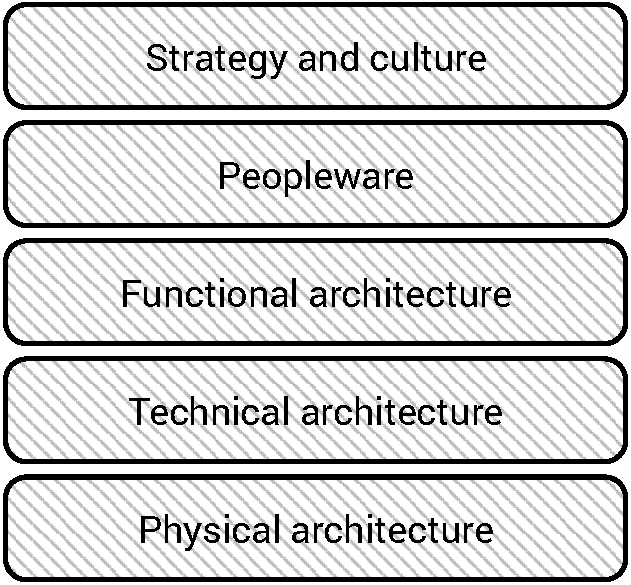
\includegraphics[width=\linewidth]{stack.pdf}
		\caption{Organisatsiooni kihiline mudel}
		\label{fig:stack}
	\end{center}
\end{marginfigure}

Peamine sõnum auditooriumist: tuleb leida tasakaal lihtsa käsutäitmise ning täiesti paindliku lahenduse vahel, kumbki ei ole soovitav.

\TODO vajab viidet N juhtumile ja stacki põhjalikku lahtikirjutust koos arutluskäiguga

\subsection{Kuidas juhtida mõistlikult ITd kui organisatsioon kui tervik ei ole mõistlikult juhitud?}
\label{sec:strategy:q3}
Elu näitab, et organisatsioone võib pikalt juhtida viisil, mida kindlasti mõistlikuks pidada ei saa. Kindlasti võib äriettevõtete langus kesta aastaid ning ka avalikus sektoris võivad demokraatlikud mehhanismid tekitada olukorra, mis tingimata juhtimislikult mõistlik ei ole. Seega tekib küsimus, kas ja kuidas mittemõistlikus organisatsioonis on võimalik tegeleda mõistliku IT juhtimisega.

Peamine sõnum auditooriumist: proovime pakkuda paremaid lahendusi (mõisnik ja banaan), seletame otsuste mõju (ajahorisondi küsimus).
\ref{sec:strategy:q1}
\TODO korralikult lahti kirjutada

\chapter{Arhitektuur}
\section{Arhitektuuri ajaloost}
Inimesed on aastatuhandeid maju ehitanud. Ja sama vana on arhietkuuri mõiste. Ka meie esivanematel oli väga selge ettekujutus, kui suur üks hea rehetare peaks olema, mis ilmakaarde vaatama ning kuidas paiknema vee suhtes. Mis see muu on, kui arhitektuur?

\begin{marginfigure}
	\begin{center}
		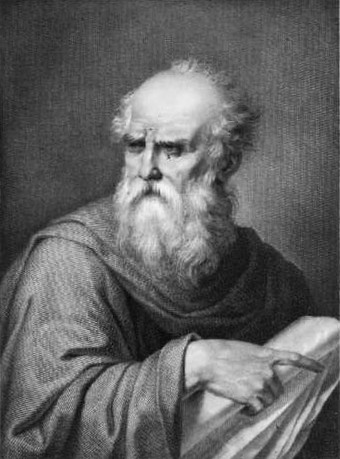
\includegraphics[width=.84\linewidth]{vitruvio.jpg}
		\caption{Marcus Vitruvius Pollio, 80-70 eKr.- 15 pKr}
		\label{fig:vitruvius}
	\end{center}
\end{marginfigure}

Siinkandis\sidenote{Induse orus tekkisid linnastud juba 2600 e.k., ilmselt tegeldi seal ka arhitektuuriga} ehk kõige kuulsamad majaehitajad olid kreeklased. Rooma impeeriumi laienemisega oli kõikjale vaja luua uusi asundusi ja kindlustatud tugipunkte. Seega oli suur vajadus ka arhitektide järele. Meie ajaarvamise alguse Rooma riigist pärinebki ehk esimene terviklik kästilus arhitektuurist\cite{pollio1914vitruvius}. 

Too Vitruviuse teos on tänaseni märkimisväärselt loetav ja aktuaalne. Samm-sammult kirjeldatakse eritüübiliste hoonete planeerimise ja konstrueerimise detaile alates üldisetest põhimõtetest (Alati ehita linna peatänav risti talviste tuulte peamise suunaga) kuni sammaste täpsete mõõtmeteni. Sellisena on tegemist tavapärasest arhitektuurist oluliselt laiema kandepinnaga teosega. Rõhk kasutaja vajadustel, juhised konteksti arvestamiseks ning tugev seos insenerikunstiga on kõik asjad, mis on tänasele tarkvaraarhitektile täpselt sama olulised kui toonasele majaehitejale. 

Ehk kõige olulisem Vitruviuse pärand on tema kolm üldist printsiipi, millele kõik ruumiga tegelevad kunstid alluma peaksid\index{Arhitektuur!Printsiibid}: tugevus (püsivus), otstarbekus, ilu.\cite{vitruviusest}. Tol ajal arvuteid polnud kuid samade printsiipide rakenduvuse vastu tänapäevases tarkvara arhitektuuris on raske vaielda. 

Viimase paarisaja aasta jooksul on arhitektuurimõte küll edasi arenenud, kuid, huvitaval kombel, ei ole esile kerkinud ühtset arhitektuuri definitsiooni. Enamasti mõeldakse arhikektuuri all millegi osiste ning nende seoste skemaatilist kirjeldust. Selline lähenemine on aga piiratud, sest räägib vähe tolle kirjelduse tekkeprotsessist või ka arhitektuuri kui sellise väärtusest. Läheb kaotsi arhitekti töö loominguline komponent. Samuti on nii mõeldes lihtne takerduda valdkondade piiridesse: arhitektuuridokumente toodetakse ju eesmärgiga ühe või teise elukutse esindajale juhiseid anda. Aga kuhu jääb tervik? 

IT strateegia kontekstis on tüüpiliselt objektiks, mida disainida, organisatsiooni tegevust toetav infosüsteem. Et sedalaadi infosüsteemide disain on olulise ärilise tähendusega, on arenenud terve tarkvara arhitektuuri haru, ettevõttearhitektuur\sidenote{Ingl. \emph{Enterprise Architecture}. Tegemist on mõnevõrra eksitava mõistega, kuna tüüpiliselt on tähelepanu ettevõtte infosüsteemide ja mitte ettevõtte kui sellise arhitektuuril}.

\section{Paradigmamuutus ettevõttearhitektuuris}
\label{sec:architecture:paradigm}
Ettevõtte arhitektuuriraamistike\index{EA} ajalugu algab 1987. aastal Zachmani klassikalise paberiga \cite{zachman1987framework}. Sellest alates on toimunud päris oluline areng, mille üldjoontes võtab kokku joonis \ref{fig:architecture:EA}. 

\begin{figure}%
	\begin{center}
		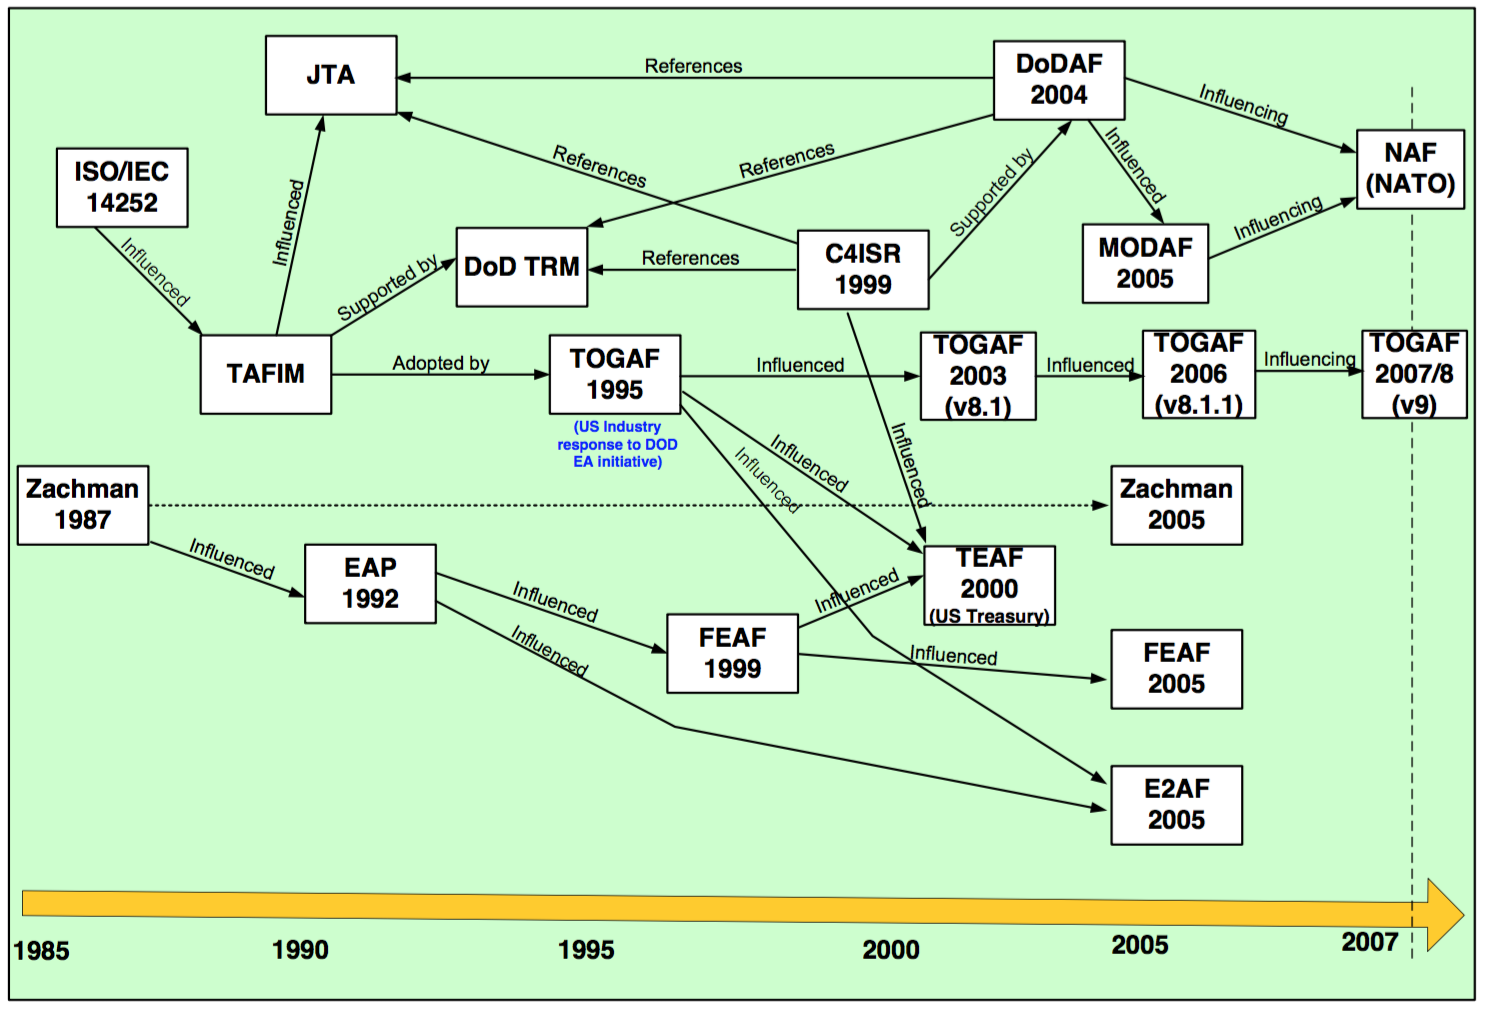
\includegraphics[width=\linewidth]{eaevolution.png}
		\caption{Arhitektuuriraamistike evolutsiooniline kontekst}
		\label{fig:architecture:EA}
	\end{center}
\end{figure}

Siit paistab nii mõndagi huvitavat. Kõigepealt on näha, et raamistikud uuenevad jämedalt viie-aastase kadentsiga. Teiseks on märgatav militaarorganisatsioonide oluline mõju. Kolmandaks näeme, et joonis lõpeb aastaga 2007. 2009. aastal on üllitatud küll DoDAF\index{DoDAF} v. 2.02 aastal 2010 kuid isegi raamistikke võrdlevat kirjandust on sel kümnendil ilmunud vähe. Siit võib järeldada, et ühel või teisel põhjusel liiguvad arhitektuuriraamistikud tehnoloogia arengust oluliselt aeglasemalt ning et valdkond on teatavas mõttes kriisis. Tõenäoliselt saavad üksikud spetsiifiliste vajadustega organisatsioonid nagu NATO või USA kaitseministeerium oma raamistikest väärtust, kuid nende rakendatavus väljaspool militaarvaldkonda on küsitav. 

Põhjusi on ilmselt mitmeid, kuid tõenäoliselt on oma roll nii organisatsioonide kui nende keskkonna keerukuse kasvul. Võib välja tuua neli eeldust, mis raamistike kuldajal sajandivahetuse paiku veel enamasti kehtisid kuid täna on tõesed järjest väiksema hulga ettevõttearhitektuurist kasu saada võivate organisatsioonide puhul.

\textbf{Organisatsioonid on kultuuriliselt, tehniliselt jne. homogeensed}. Isegi, kui tegu oli rahvusvaheliste organisatsioonidega, ei pruukinud eraldiseisvad üksused olla tihedalt integreeritud. Integratsioon eeldab kommunikatsiooni ja seda on ilma internetita keeruline efektiivselt korraldada. \citeauthor{cfmcommnetworks}\cite{cfmcommnetworks} näitab, et keskmine teadmustöötaja USAs suhtles veel sajandivahetuse paiku isegi e-posti olemasolul vaid temast väga piiratud füüsilises raadiuses olevate inimestega. See tähendas, et mitmesuguseid kultuurilisi, tehnilisi vms. piire tuli igapäevases töös ületada suhteliselt harva. Tänapäeval on ka Eestis vähegi edukamate ettevõtete kliendid ja töötajad maailmas laiali ning meie sotsiaalsed, juriidilised ja ärilised suhted on üha enam piiriülesed\sidenote{Maailm tundub üha väiksemaks jäävat. Tavapäraselt arvatakse, et globaalse suhtevõrgustiku keskmine kaugus kahe inimese vahel on kuus. Facebook on leidnud selle numbri aastal 2015 olevat 3.57, sama number aastal 2011 oli 3.74\citep{backstrom2012four}}. Otsuste tegemisel ei saa enam eeldada, et otsuse täideviijat õnnestub efektiivselt mõjutada ning et tollel täideviijal, kui kohaliku konteksti tundjal, ei ole head põhjust otsuse vastu tõrkuda. Samuti on järjest ohtlikum eeldada homogeenset organisatsiooni kultuuri\index{Kultuur} või et selle komponendid oleksid isegi sarnased.

\textbf{Organisatsioonilised ja juriidilised piirid on selgelt määratletud}. Klassikaliselt on organisatsioonide ning rahvusriikide piirid ning vastutusala selgelt määratletud. Iga organisatsioon ajab äri suhteliselt iseseisvalt ning iga rahvusriik omab suveräänset kontrolli oma territooriumi üle. Tänapäevases globaliseeruvas maailmas ei ole kumbki enam tõsi. Ettevõtted on üha enam osad rahvusvahelisest tarnijate ja klientide võrgustikust, mida läbivad tihedalt integreeritud tarneahelad. Rahvusriigid aga üritavad leida oma kohta olukorras, kus kriitiline mass sotsiaalseid, ärilisi ja juriidilisi suhteid on riigipire ületavad. Vaid tõeliselt suured ettevõtted nagu Apple suudavad väärtusahelat pidi üles- ja allapoole märkimisväärset mõju avaldada. Ülejäänud peavad leppima keeruliste sõltuvustega kolmandatest osapooltest. 

\textbf{Organisatsioonid on suhteliselt sõltumatud globaalsetest probleemidest}. Kuigi inimkonna kui terviku ees seisvate probleemide eskaleerumisest on räägitud juba alates möödunud sajandi seitsmekümnendatest \cite{forrester1971world}, hakkavad toona mudelite ennustatud kriisid pärale jõudma alles nüüd. Globaliseeruvas maailmas ei ole rahvastiku kasvu, kliimamuutuse, ökoloogilise katastroofi ning teiste probleemide eest kellelgi pääsu. Kui inimkond probleemidega toime ei tule, kannatavad kõik. Kui aga tuleb, on selge eelis muutustega kaasa läinud ning probleeme õigesti mõttestanud ettevõtetel. 

\textbf{Kasutusel on selgepiirilised kontrollitult toimivad infosüsteemid}. Eestis lõi omal ajal laineid Tiigrihüppe programm, mille oluline rõhk oli inimeste õpetamisel arvutit kasutama. Ja põhjusega: arvutid ja tarkvara olid keerulised ning vajasid vähegi komplekssema ülesannete lahendamiseks eriväljaõppega kasutajaid.  Infosüsteemid täitsid organisatsioonis kindlat rolli ning suhestusid teiste äriprotsessi osadega suhteliselt kitsa tehnoloogiapreestrite kasti vahendusel. Tänapäeval on tiigrihüpe oma rolli täitnud ning nutiseadme kasutamiseks on ka kolme-aastane piisavalt nutikas. Tarkvara ning eri kommunikatsioonitehnoloogiad on üha enam universaalselt kasutatavad ning imbunud organisatsioonide toimimise kõigisse aspektidesse sotsiaalsetest suhetest äriprotsessi juhtimiseni. 

Ehk, ettevõttearhitektuuri kuldajast alates on organisatsioonide toimimise eeldused põhjalikult raputada saanud. Kirjeldatud muutused tähendavad ühest küljest keerukuse olulist kasvu ja teisalt piiride hävustumist ettevõtte kui sellise, teda toetav infosüsteemi ning nende mõlema toimimise füüsilise konteksti vahel. Seega on vaja lähenemist, mis võimaldaks need kolm tervikuks siduda.

\section{Moodne vaade arhitektuurile}
\label{sec:arch:fcc}
Üheks võimaluseks ületada klassikalise lähenemise kitsaskohad on kasutada süsteemimõtlemist\index{Süsteemimõtlemine}. Süsteemimõtlemine\sidenote{Ingl. \emph{system thinking}. Mõtteviisi juured on eelmise sajandi alguse holistiliste mõtlejate töödes kuid oma praeguse kuju on nad saanud Jay Forresteri ja Peter Senge töödes} on lihtsalt mõtlemine olukorrast või probleemist kui süsteemist. Suhteliselt lihtsasti määratletava lähenemise võti on holismis: uuritakse süsteemi kui tervikut sõltumata tehnoloogiatest, distsipliinidest või vastutusvaldkondadest. Kui tavapärane lähenemine tarkvara arhitektuurile seab fookusse tarkvara siis süsteemimõtlemisest tulenev vaade käsitleb tark- ja riistvara, kasutajaid, organisatsioone jms. võrdväärsetena.

\begin{marginfigure}
	\begin{center}
		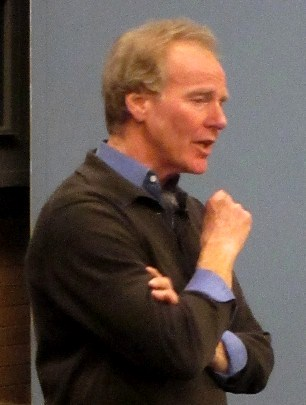
\includegraphics[height=3.3cm]{Peter_Senge_at_Quest_to_Learn.jpg}
		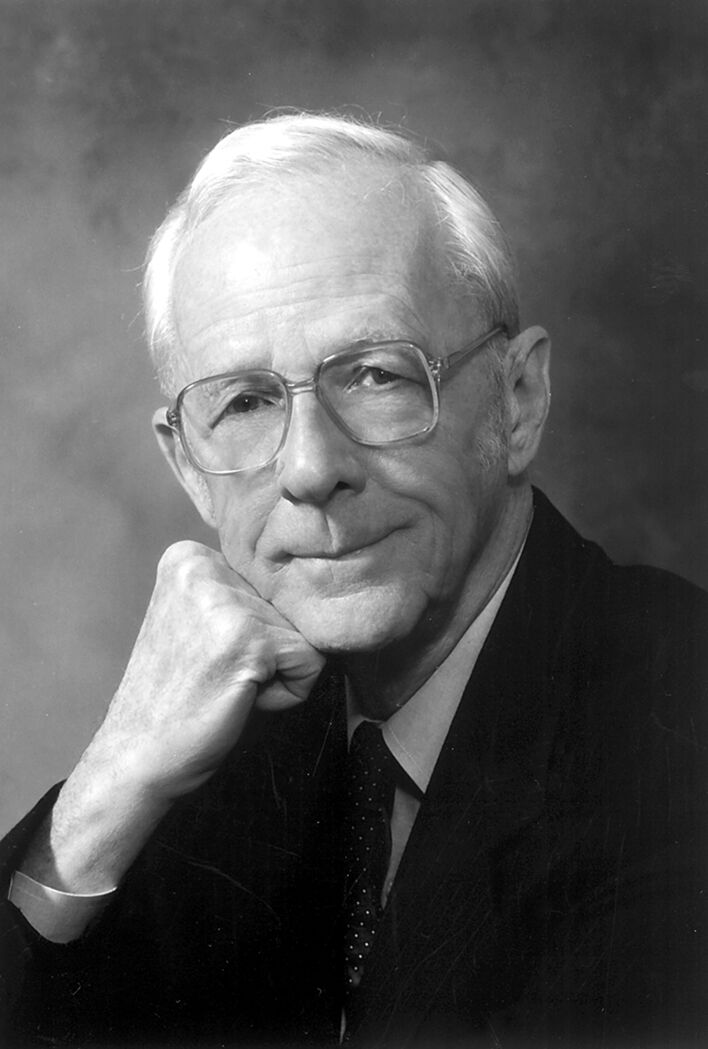
\includegraphics[height=3.3cm]{jayforrester.jpg}
		\caption{Peter Senge\index{Senge, Peter} (By Beyond My Ken - Own work, GFDL, \url{https://commons.wikimedia.org/w/index.php?curid=24627572}) ja Jay Forrester\index{Forrester, Jay}}
		\label{fig:legendid}
	\end{center}
\end{marginfigure}


\begin{marginfigure}
	\begin{center}
		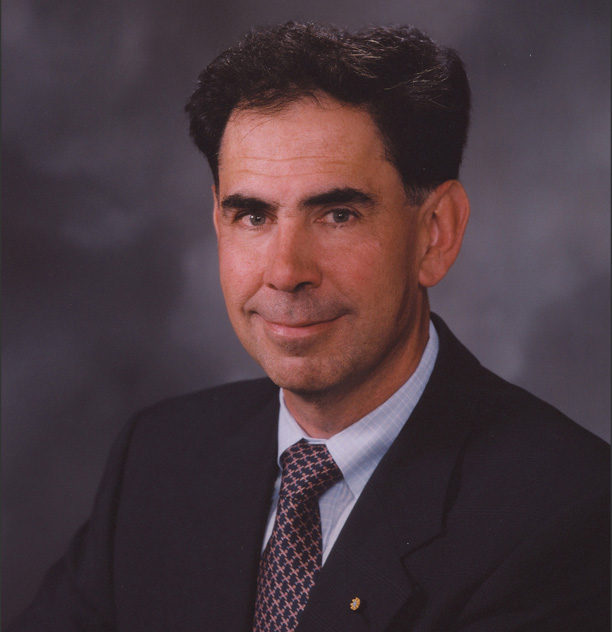
\includegraphics[height=3.3cm]{MIT-Ed-Crawley_0.jpg}
		\caption{Edward Crawley}
		\label{fig:ed}
	\end{center}
	Kauaaegne MIT professor Ed Crawley\index{Crawley, Edward} on töötanud koos NASAga ISSi kallal, asutanud mitmeid ettevõtteid ning olnud Skoltechi esimene rektor. Prof. Crawley süsteemiarhitektuuri üks vaieldamatuid suurkujusid maailmas.
\end{marginfigure}

Edward Crawley defineerib süsteemi arhitektuuri\index{Süsteem!Arhitektuur}\index{Arhitektuur!Definitsioon} nii:
\quote{The embodiment of concept, and the allocation of physical/informational function to elements of form, and definition of interfaces among the elements and with the surrounding context.}

Vaadakem seda definitsiooni lähemalt. 

Esmalt rõhtutatakse kontseptsiooni mõistet. Kontpsetsioon\index{Kontseptsioon!Definitsioon} on süsteemi peamine mõttemudel ja lähenemisviis, mis seob funktsiooni just selle konkreetse lahendusega. On tähenduslik, et seda mainitakse esimesena: just see osis seob definitsiooni tervikuks olles samas ka mainitud mõistetest kõige hoomamatum. Funktsioon\index{Funktsioon!Definitsioon} on see, mida süsteem \emph{teeb}. Siit tuleneb süsteemi kasulikkus ja ta on teenitult paigutatud järgmisele kohale. Vorm\index{Vorm!Definitsioon} on see, mis süsteem \emph{on}. Siit tulenevad süsteemiga seotud kulud. Näeme, et süsteemi puhul on oluline kolmik vorm, funktsioon ja kontseptsioon ning et tegu on üldise definitsiooniga. Ei funktsiooni ega vormi kohta ei öelda muud, kui et neil on mingisugune sisemine struktuur. Järgnevalt mainitakse liideseid\index{Liidesed} elementide vahel. Ehk, süsteemi puhul on oluline ka viis, kuidas tema elemendid suhestuvad nii omavahel kui ka ümbritseva keskkonnaga.

\section{Printsiipidest}
\index{Arhitektuur!Printsiibid}
Arhitektuuriga süvitsi tegelemisel on hea mõte pidada printsiipide päevikut. Arhitektuuris on mõttemudelil oluline koht ja seega on mõistlik tegeleda oma isikliku mõttemudeli arendamise ning dokumenteerimisega. Printsiibipäevik on üks viis seda teha. Printsiip on miski, mis tundub kehtivat alati ning mis ei sõltu teistest. Teatavas mõttes on tegemist universaalse tõega. Üheks näiteks printsiipidest arvutivõrkude vallas on RFC 1925\cite{callon1996rfc}. Printsiibipäeviku mõte on selles, et iga kord, kui igapäevases töös tundub mõni printsiip silma jäävat, kirjutatakse see jalamaid üles. Perioodiliselt vaadatakse päevik üle lootuses destilleerida kirja pandust veel universaalsemaid ja üldisemaid põhimõtteid. Üks näide sellisest päevikust on \cite{archprinciples}. 

Arhitektuuri printsiipide osas tuleb jälle viidata \citeauthor{crawley2015systems} tööle. Ta peab printsiipe nii oluliseks teadmuse jagamise vahendiks, et on need paigutanud raamatu sisekaanele. Üheks näiteks tema printsiipidest on arhitekti rolli printsiip \enquote{Arhitekti roll on vähendada ebamäärasust, fokusseerida loovust ja vähendada keerukust}\cite{crawley2015systems}.

\section{Emergentsusest}
Ingliskeelsel terminil \emph{emergence}\index{Emergents} on eesti keeles vasteks emergentsus\footnote{Vahel öeldakse ka ``ilmnemine``: Emergent behaviour tõlgitakse kui \enquote{ilmnev käitumine}}. Nii tähistatakse süsteemi omadust, mis seisneb millegi ilmnemises tänu mingitele muudele süsteemi omadustele. Arhitektuuri kontekstis on emergentsus süsteemide omadus lisaks disaini kaudu eesmärgiks seatud omadustele ka teiste omaduste ilmnemiseks. Tüüpiline emergentne omadus on võime inimesi tappa: suur hulk tehnoloogiaid alates tulest ja lõpetades tuumareaktsiooniga on mingil hetkel osutunud efektiivseks vaenlastest vabanemise vahendiks. Esimene nuga ei olnud mõledud mõrvaks kuid seda on nii aegade algusest kasutatud. Tüüpiliselt ei ole probleem mitte niivõrd süsteemi enda emergentsed omadused vaid emergents, mis sünnib eri objektide kombinatsioonist. Laua funktsioon on toetada asju. Joonlaua funktsioon on sirgeid jooni tõmmata. Kui aga asetada joonlaud poolenisti lauale, oleme saanud, sõltuvalt vaatepunktist, kas muusikariista või inimeste ärritamise vahendi. 

Mitte kõik emergentsed omadused ei ole lihtsalt ebasoovitavad või ootamatud \cite{emergence} toob häid näiteid sellest, kuidas pilvelõhkujad oma arhitektuuriga lausa inimesi ohustada võivad.

\section{Süsteemi piiride probleem}
\label{sec:boundary}
\index{Süsteem!Piirid}
Kui rääkida süsteemist, tekib alati küsimus süsteemi piiridest: kus algab meie kontrolli all olev ala ja kus ta lõpeb? \cite{wood2013framework} räägib osapoolte kaasamisest ning probleemipüstituse juures küsib õigesti: kuidas saada kontrolli alla konkreetse rakenduse teise ja kolmanda järgu efektid? Ehk, kuidas vältida projekti ebaõnnestumist, sest temast tõusis kahju meie olulise kliendi olulisele partnerile? Lahendusteks pakutakse osapoolte omavaheliste suhete analüüsi sotsiaalvõrkude puhul kasutatavate meetoditega. Siiski ei anta ka siin vastust küsimusele kirjeldatud võrgu piiridest: ei ole selge, kuidas otsustatakse, keda võrku kaasata ja keda mitte (kas kliendi kliendi klient on ka oluline?). 

Lisaks konkreetsele osapoolte kaardistamise raamistikule annab artikkel ka mõningase ülevaate erinevatest EA raamistikest.

	
\section{Küsimusi aruteluks}
\subsection{Millist väärtust loob arhitektuuriga tegelemine?}
Arhitektuur tundub oluline kuid samas on ka selge, et arhitekti mitteilmumine tööle ei põhjusta tavaliselt kohest kadu produktiivsuses. Arhitekti töö väärtust on mõnevõrra keeruline hinnata. 

Peamine sõnum auditooriumist: mõjuanalüüs, suur pilt, optimiseerimine/kulud
\TODO kirjuta lahti

\subsection{Kui palju erineb süsteemimõtlemisele tuginev mudel harjumuspärasest?}
Palju.
\TODO Näide testimise modelleerimisest. Lineaarne vs. mittelineaarne lähenemine

\chapter{Äriplaan}
\section{Arendus- ja halduskuludest}
\label{sec:kulud}
Laias laastus võib öelda, et kulud arendusele jagunevad kuludeks\index{Kulud!Arendus}index{Kulud!Haldus}, mis tarnivad uut funktsionaalsust (ning mida tavaliselt tajutakse kui uut väärtust\index{Väärtus} lisavatena) ning kuludeks, mis lähevad olemasoleva muutmiseks või parandamiseks. Neist esimesed lisavad selgesti halduskoormust ja halduskulusid luues uusi rakendusi, mida tuleb hallata, millede teenustase tuleb tagada. Teised aga võivad (aga ei pruugi) halduskulusid vähendada näiteks tehnilist tehnilist võlga likvideerides. Arenduskulusid võib vaadata ka keerukuse vaatepunktist: esimest liiki kulud suurendavad, teised võivad aga keerukust vähendada. Kokkuvõte kuludest ja nende mõjudest on toodud tabelis \ref{tab:arendus}.

\begin{table}
	\begin{center}
		\begin{tabular}{p{2.8cm}p{1.7cm}p{1.5cm}p{2cm}}
		\toprule
Kulu & Mõju haldus\-kuludele & Mõju tajutud väärtusele & Mõju \mbox{keerukusele} \\
\midrule

Uue funktsionaaluse \mbox{lisamine} & Selgesti \mbox{suurendab} & Selgesti \mbox{suurendab} & Selgesti \mbox{suurendab} \\
\addlinespace
Olemasoleva muutmine või parandamine & Neutraalne või vähendab & Reeglina \mbox{neutraalne} & Neutraalne, \mbox{pigem} vähendab \\

\bottomrule
		\end{tabular}
		\caption{Kokkuvõte arenduskulude mõjust}
		\label{tab:arendus}
	\end{center}
\end{table}

Siit tuleneb oluline tõdemus: arenduskulud, mis suurendavad tajutud väärtust tekitavad juurde ka halduskoormust ja lisavad keerukust viies seega alla organisatsiooni võime tulevikus uut väärtust lisada. Võtmeks tupikust välja on sõna "tajutud". Muutes viisi, kuidas organisatsioon tajub ITst tulenevat väärtust on võiamlik saavutada tellija arusaam IT kulude dünaamikast.

Nagu kõik investeeringud, on investeeringud ITsse finantsjuhtimise objektiks. Investeeringud amortiseeritakse teatud perioodi  jooksul ja kulud kaetakse jooksvast eelarvest. Kui äriorganisatsioonil on fikseeritud aastane kulueelarve IT suunas, tekib kiusatud suuremahulised projektid teha investeeringutena ning hiljem katta vaid amortisatsioonikulusid. Selline lähenemine tuleneb kogemusest materiaalse põhivaraga, kus põhivara haldamiseks tehtavad kulutused on oluliselt väiksemad amortisatsioonikuludest. Investeerides näiteks mõnda masinasse, see kulub kuni ei ole enam mõistlikult kasutatav. Jah, igakuiselt tuleb maksta hooldusarveid, kuid need on tüüpiliselt oluliselt väiksemad, kui liisingmakse. Samuti on hoolduskulud tavaliselt äriplaanis juba toote omahinnana arvesse võetud. 

Infosüsteemide puhul on olukord oluliselt erinev. Pärast algset investeeringut tarkvara loomisse, hakkavad jooksvalt tekkima vähemalt järgmised kulud:
\begin{description}
	\item[Serverid, võrguseadmed ja nende majutus] Serverid amortiseeruvad, neid peab hoidma jahedas valvatavas ruumis ning nad võtavad elektrit
	\item[Süsteemi monitooring] Keerukad infosüsteemid vajavad tüüpiliselt mingit jälgimist, halvemal juhul 24/7. 
	\item[Klienditugi] Reeglina vajab infosüsteem teatud tuge kliendile. Olgu selleks õiguste lisamine ja eemaldamine, finantsaasta vahetusega seotud tegevused, tavapärane tõrkeotsing või lihtne kliendi õpetamine, peab leiduma keegi, kes vajadusel süsteemi kapoti alla vaatab
	\item[Internetiühendus] Infosüsteemi kasutatakse reeglina läbi internetiühenduse. Korralik internetiühendus maksab raha ning see kulu ei pruugi olla väike. Keerukamatel juhtudel lisanduvad veel kulud CDNile\sidenote{CDN - \emph{Content Delivery Network}. Süsteem, mis vähendab kasutaja poolt tajutud latentsi tehes süsteemi osad kättesaadavaks lõppkasutajale interneti topoloogia mõttes soodsates asukohtades} ja muule sellisele
	\item[Turvateenused ja riistvara] Infosüsteemid vajavad kaitset ning vastavat riist- ja tarkvara ning teenuseid on turul saadaval. Turvaseadmed on näiteks tulemüürid ja riistvaralised SSL-kiirendid ning teenusena võib sisse osta kõike alates operatsioonisüsteemi paikamisest kuni teenustõrkerünnete vastasest taristust  
	\item[Infoturve] Lisaks riistvarale ja tarkvarale vajab iga infosüsteem pidevalt infotehnoloogilist tähelepanu. Küberruumis kasutatavad ründevahendid arenevad pidevalt ning nii teie loodud tarkvaras kui seda toetavates süsteemides tuvastatakse pidevalt turvavigu. Nende vigade järgimine ning tarkvara uuendamine vajavad küllalt spetsiifilist kompetentsti.
\end{description}

Kõigil neil kuludel on kolm omadust:
\begin{enumerate}
	\item Nad on üksteisest raskesti konkreetsele süsteemile allkoeeritavad. Kui organisatsioonil juba on 24/7 monitooringuvõimekus, eeldab see hulka hästi organiseeritud inimesi. On üsna keeruline hinnata, kui palju tööd lisab neile iga konkreetne uus lahendus. Inimene on öösel telefonivalves ju igal juhul? Kui suure osa serveriruumi külmast õhust võtavad just konkreetse süsteemi serverid?
	\item Nad on arenduskulude\sidenote{Mis omakorda genereerivad halduskulusid käivitades omaette tagasiside} kaudu tagasisidestatud. Monitooring ja klienditugi võivad avastada süsteemist parandamist vajava vea, infoturve võib leida, et süsteemi riskide aktsepteerivale tasemele viimiseks on vaja teha arendustööd. Süsteemi piisava jõudluse tagamiseks ei pruugi olla võimalik enam riistvara lisada. Kõik muutused tarkvaras aga tekitavad uusi vigu, vajadust klienti toetada, jõnkse monitooringule, tegevust infoturbele jne. 
\end{enumerate}

Kõik need kulud moodustavad tüüpiliselt oluliselt suurema ning raskemini hinnatava\sidenote{Siit tuleb üks olulisi pilveteenuste\index{Pilveteenused} võlusid. Kuna need võimaldavad ressursikasutust täpselt hinnata, on nende abil võimalik süsteemide kulutatavat oluliselt selgemini eristada. Kasu tuleb nii privaat- kui avaliku pilve puhul.} protsendi algsest investeeringust, kui materiaalse põhivara puhul. 

Kui pildile lisada veel asjaolu, et tehnoloogia kipub ajas vananema suurendades halduskulusid\sidenote{Vt. \nameref{sec:rooste}}, siis ei ole üldse selge, milline mõju saab olema arendusprojekti amortiseerimisel (hoides kulubaasi stabiilsena kuid vähendades kulusid jooksvale haldusele ning arendusele) või kohe kulusse kandmisel.

Küsimus arenduskulude juhtimisest on eriti oluline avalikus sektoris. Ühest küljest puudub siin kasumlikkuse surve\sidenote{18f, USA föderaalvalitsuse digitaalagentuuri blog on hea allikas avaliku sektori it-probleeme lahkavate artiklite osas. \url{https://18f.gsa.gov/2016/02/23/software-maintenance-is-an-anti-pattern/} on selle lõigu inspiratsiooniks} ja teisalt on kulud ja investeeringud reeglina rangelt eraldatud. Mõlemad seavad süsteemi hooldamiseks tehtavad kulutused tugeva surve alla: esimene tekitab tunde, et hoolduskulud on ebavajalikud ja teine võimaldab taotleda finantseeringut projektidele, mille hooldamiseks puuduvad vahendid. Nii tekib olukord, kus oluline investeering ei tooda puuduva hoolitsuse tõttu maksumaksjale piisavalt väärtust. 

Probleemi ületamiseks pakub 18f, et igal süsteemil peaks käivitusperioodi lõppedes tekkima eri osapoolte esindajatest (sh. arendajad) koosnev meeskond, mis tegeleb järgmisega
\begin{description}
	\item[Kasutaja vajadus] Kes süsteemi kasutab? Kas kasutajate rühm kattub algse sihtrühmaga? Kui ei, siis kuidas kasutajad oma vajadusi rahuldavad?
	\item[Konkuretsianalüüs] Millised meie omale sarnased süsteemid turul eksisteerivad ning kas me peaksime neid täiendama (ehk, katma funktsionaalsust, mida nemad ei kata), asendama (pakkuma paremat kvaliteeti ja rohkem funktsionaalsust) või kasutama (sulgema oma teenuse ning ostma selle sisse)
	\item[Kasutatavustestid] Kuidas olemasolevad kasutajad meie süsteemi kasutades käituvad, milline on üldine kasutajakogemus ning kas seda saab parandada?
	\item[Arendussaba sugemine]\sidenote{\enquote{Arendussaba} on maakeelne vaste ingliskeelsele terminile \enquote{Backlog}. Mis oma olemuselt on süsteemi teadaolevate defektide, probleemide ja arendussoovide nimekiri. Mida, on ütlematagi selge, on mõistlik pidada ning aegajalt puhastada, ehk sugeda, eemaldades sealt aegunu ning ebavajaliku.}\index{Arendussaba} Millised read nimekirjas on ühe (millise?) probleemi sümptomid? Millised probleemid suudame olemasolevate vahendite raames parandada ja millised mitte?
	\item[Meetrikate järgimine] Kas NPS\index{Net Promoter Score}\sidenote{\emph{NPS - Net Promoter Score} on kõige lihtsamas versioonis kasutajate keskmine vastus küsimusele \enquote{Kui tõenäoliselt soovitaksid käesolevat teenust sõbrale või kolleegile?}} või mõne muu meetrika väärtus vastab meie ootustele, soovidele ja vajadustele?
\end{description}

\section{Arhitektuur ja äri}
Toote või teenuse arhitektuur mõjutab otseselt orgranisatsiooni ärilist positsiooni. Crawley järgi on igal süsteemil kolm olulist aspekti: vorm, funktsioon ja kontseptsioon (vt. \nameref{sec:arch:fcc}).

Toote või teenuse väärtus tuleneb tema funktsioonist: mida täpsemalt vajadust täidetakse ning mida põletavam too vajadus, seda väärtuslikum toode või teenus. Süsteemiga seotud kulud tulenevad aga kogu elutsükli jooksul vormist: vormi loomiseks tuleb hankida materialid, viia läbi tootmine ning lõpuks utiliseerimine. Järelikult tuleneb vormi ja funktsiooni vahekorrast (mida suuresti määratleb kontseptsioon), süsteemi võimekus väärtust lisada. 

\begin{marginfigure}
	\begin{center}
		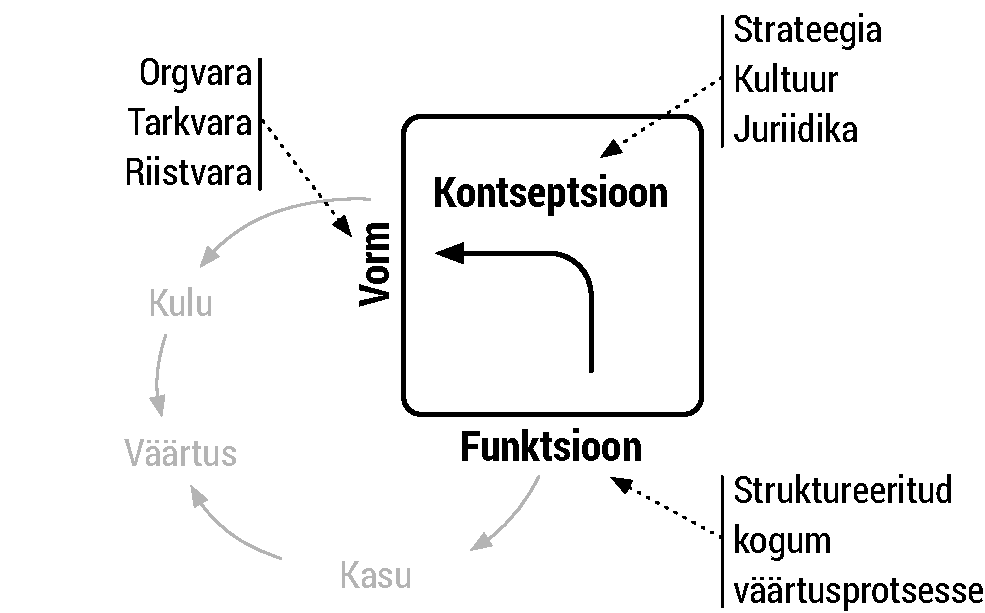
\includegraphics[width=\linewidth]{ffc_profit.pdf}
		\caption{Organisatsiooni eri aspektide seosed omavahel ja organnisatsioon majanduseduga}
		\label{fig:arh}
	\end{center}
\end{marginfigure}

Toote või teenuse võimest väärtust lisada tuleneb aga organisatsiooni kui terviku väärtuse lisamise võime ning seega ka majanduslik jätkusuutlikkus. 

Kasumi ja arhitektuuri seoseid illustreerivaid näiteid on nii kaugemast kui lähemast minevikust mitmeid. Positiivsena tasub esile tuua Black \& Deckeri strateegilist tooteinnovatsiooni seitsmekümnendatel ning Volkswageni platvormistrateegiat. Negatiivsena on üks tuntumaid General Motorsi lähenemine platvormidele. 


\section{Ettevõtte arhitektuurist}
Traditsioonilised EA\footnote{ingl. \emph{Enterprise Architecture}}\index{EA} raamistikud räägivad palju äriarhitektuurist kuid teevad seda abstraktselt. Detailidesse minnakse reeglina vaid infosüsteemide puhul. Paremal juhul eeldadatakse, et muude organisatsiooni aspektide juhtimine võtab üle IT terminoloogia, lähenemise ja mõtteviisi. Organisatsioon koosneb aga liiga paljudest eri taustaga inimeste eri fookusega vastutusaladest, et oleks lootust neile kõigile üht metoodikat rakendada.  Seetõttu on EA kui distsipliin end sageli diskrediteerinud jäädes kageks nii ärist (kes lihtsalt mõtlevad oma probleemidest teisel viisil) kui inseneridest (kes peavad igapäevaselt tegelema ärilise keerukuse valamisega infosüsteemidesse). \sidenote{Vaata ka \nameref{sec:architecture:paradigm}}

Mida siis teha? Soovitusi annab \cite{fowlerlean}. Artiklis on oluline alltekst: kuigi räägitakse arhitekti rollist agiilses organisatsioonis, isegi ei mainita võimalust, et organisatsioon agiilseks \emph{ei muutuks}. Arhitekti roll kaasaegses organisatsioonis peab muutuma. Otsuste tegijast otsuste toetajaks. Suuna andjast sildade ehitajaks. Õpetajast õppiva kogukonna keskmeks. 

\section{Küsimusi aruteluks}
\subsection{Kuidas seletada kliendile, et tema eilsel otsusel on mõju tema tänasele kulubaasile?}
\label{sec:business:q1}
Inimesed, tundub, ei suuda hästi siduda põhjust ja tagajärge. Kindlasti on üheks põhjuseks meie vajadus säilitada positiivset minapilti (\enquote{Ma olen ülekaalus, kuna mu geneetika on selline, mitte seepärast, et ma ei suuda end söömisel ohjeldada}) kuid tõenäoliselt ka evolutsioonilised faktorid. Meid ümbritsev maailm on äärmiselt mittelineaarne ning põhjuse seos tagajärjega muutub aja möödudes järjest ebaselgemaks. 

Kuidas ka ei oleks, inimeste esimene järeldus probleemi põhjuste osas ei ole reeglina endogeenne. Kuigi teooria näitab, et probleemid on harva eksogeensed. 

Ehk, kliendi käitumine ei ole mitte puuduliku personalipoliitika või isikliku küündimatuse tulemus vaid inimesed üldiselt nii käituvadki. Siinkohal olekski lihtne panna punkt, lugeda kogu probleem inimloomuse tõttu lahendamatuks. Siiski on organisatsioon tervikuna keeruline dünaamiline süsteem mille emergentse käitumisena kliendi lühiajalist fookust ka seletada saab. 

\begin{marginfigure}
	\begin{center}
		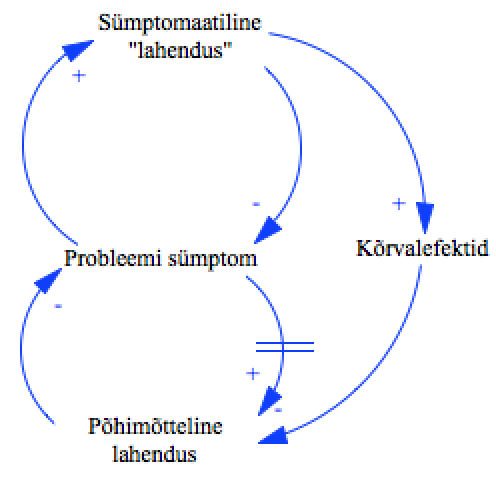
\includegraphics[width=\linewidth]{shiftingburden.png}
		\caption{Koorma nihutamise arhtetüüp.}
		Allikas: Peter Senge
		\label{fig:shifting}
	\end{center}
\end{marginfigure}

Juba viidatud Peter Senge kirjeldab oma raamatus\cite{senge19905th} tervert rida süsteemiarhetüüpe, mis kirjeldavad ettevõtetes ette tulevaid tüüp-probleeme. Üks neist on \enquote{koorma nihutamine}. Juurprobleemiga tegelemise asemel tegeletakse sümptomitega, kuni võimekus päris probleemiga tegeleda või seda isegi ära tunda kaob. Selline käitumine tõesti tihti klienti ka iseloomustab. Kuna juurprobleem (infosüsteemi kõrge hoodlusvajadus elutsükli käigus) ei ole lihtsasti lahendatav, tegeletakse üha uue funktsionaalsuse tellimisega (mis läheb ajas seda kallimaks, mida halvemini hooldatud meie infosüsteem on) kuni kogu kupatus kuulutatakse hallatamatuks, asendatakse uuega ning tsükkel algab otsast.

Senge ütleb, et sellisel puhul ei ole muud väljapääsu, kui tuumprobleemile silma vaatamine. Äriplaanid on liiga optimistlikud (sest jooksvad kulud on nende keerulise struktuuri tõttu raskesti hinnatavad ja ebameeldivalt suured) ja organisatsiooni kulujuhtimine ebapiisav (sest paljud materiaalse põhivara puhul toimivad skeemid immateriaalse puhul hästi ei toimi). Infosüsteem on pigem loom, kelle eest sa taltsutamise järel vastutad, mitte oma amortisatsiooni lõpu poole tiksuv masin.

\chapter{Tarkvaratehnika}
\section{Kokkuhoiust programmeerijatelt}
\label{sec:kokkuhoid}
Joel ütleb õigesti, et programmeerijate arendamiselt kokku hoida ei ole mõistlik. Sama kehtib ka teiste valdkondade inimeste puhul, kuid programmerijate töö on teiste omast suhteliselt info- ja teadmismahukam.

Valest kohast kokku hoitud raha (või värbamisel tehtud vead) võivad viia järgmise tagasisideni (vt. joonis \ref{fig:kokkuhoid}\footnote{Pluss-märk noolel ei tähenda mitte positiivset mõju vaid seda, et muutujad liiguvad samas suunas: ühe tõusule järgneb teise tõus ja langusele langus}):
\begin{enumerate}
	\item Koodi kvaliteet on madal
	\item Mistõttu kulub suhteliselt rohkem raha vigadega tegelemiseks ja teenitakse vähem
	\item Mis viib alla ettevõtte võimekuse inimestesse investeerida
	\item Mispeale langeb inimeste kompetentsitase veelgi (tehnoloogia ju areneb)
	\item Madalad kompetentsid viivad aga madalale koodi kvaliteedi
\end{enumerate}

Eesti IT-ettevõtted jagunevad ITLi andmetel suhteliselt radikaalselt kaheks: suured ning kasumlikud ning väikesed ja virelevad. Seda veelahet võib seletada läbi selle, kellel on õnnestunud tsükkel mis pidi tööle panna sest, muidugi, kehtib ka vastupidine. Kõrge koodi kvaliteet viib suuremate sissetulekuteni jne.

\begin{marginfigure}
		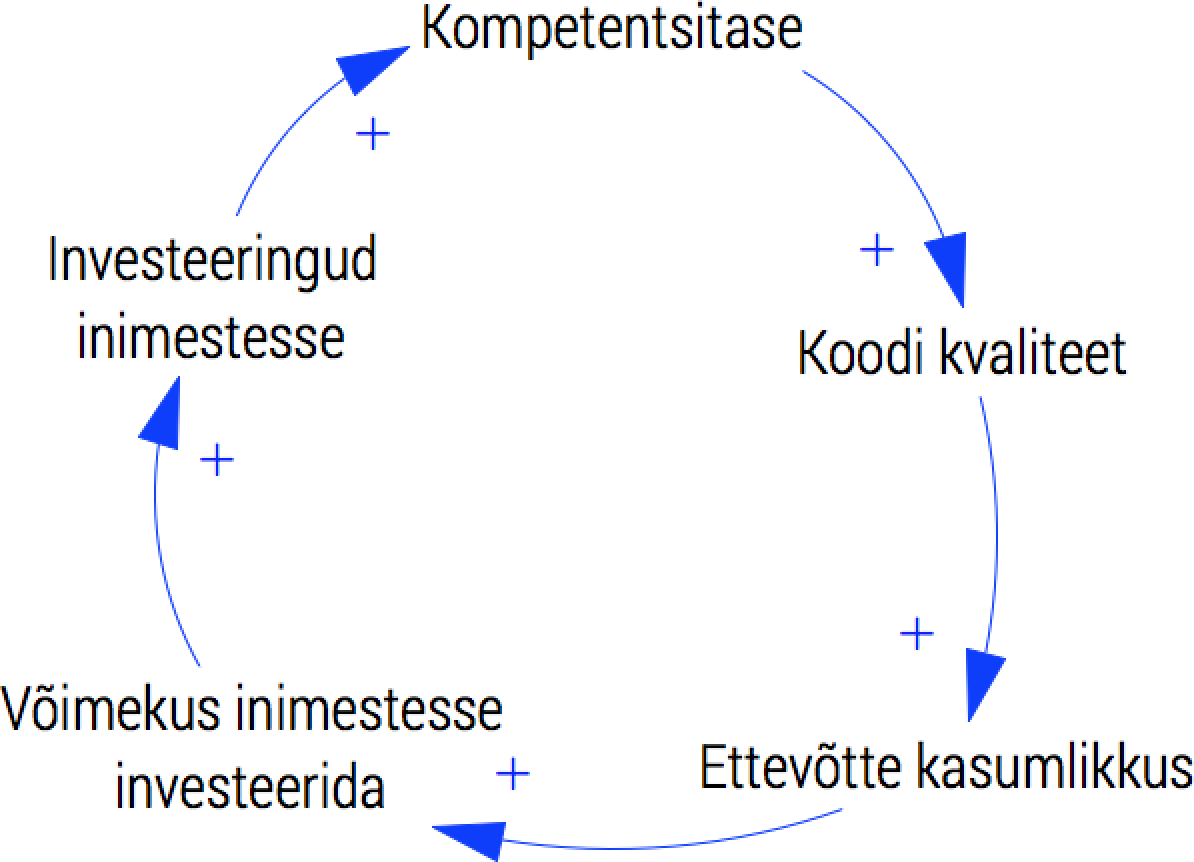
\includegraphics[width=\linewidth]{kvaliteet.png}
		\caption{Kompetentside ja kokkuhoiu seos tagasisides}
		\label{fig:kokkuhoid}
\end{marginfigure}

\section{Kood ei roosteta. Või siiski?}
\label{sec:rooste}
Joel Spolsky\index{Spolsky, Joel} ütleb, et reeglina on väga halb mõte oma koodibaasi ümber kirjutada, sest kood ju "ei roosteta" \citep{joelrust}. Ta toob mitu näidet väga ebameeldivate tagajärgedega ümber-kirjutamis ettevõtmiste kohta ning, tõesti, neid on ka siinkirjutaja praktikas mitmeid ette tulnud. Põhjuseid on mitmeid, peamiseks ehk paratamatu teadmuskadu: iga tükki koodi on juba enne rakenduse valmimist kümneid kui mitte sadu kordi muudetud ja parandatud\sidenote{Seejuures parandatud vigu me teame. Aga mis saab vigadest, mida kunagi eri raporteerita, millest me definitsiooni järgi midagi ei tea kuid millega kasutajad ja partnerid elama on õppinud?} parandamaks vigu, ületamaks nõuete ebatäielikkust jne. Nii kaob igasugune võimalus hinnata, kas kood on selline, nagu ta on, põhjusega või põhjuseta. Rääkimata analüüsist, kas põhjus jätkuvalt kehtib. Miks siis tekib vahel siiski kihu asju ümber teha ning miks on Eestis kehtestatud \emph{no legacy policy}?

Ühest küljest on asja taga kindlasti programmeerijad. Nagu Spolsky õigesti osundab, on koodi lugemine palju keerulisem, kui selle kirjutamine. Seega, eriti kui tegu on kellegi teise koodiga, on programmeerijale oluliselt lihtsam kirjutada uus kood kui üritada vanast aru saada. Loomulikult tõlgitakse vahe rahanumbriks ning uue süsteemi ehitamine võib vana turgutamisest oluliselt odavam näida. Erinevalt uue süsteemi ehitamisest, ei ole vana muutmine kergesti hinnatav ning tellija ees on kas väike fikseeritud number ebamäärase kahjuga või suur riskantne number ebamäärase tuluga. 

Teisalt võib ümberkirjutamissoovi taga olla lihtne äriliste riskide vähendamine. Vana kood peidab endas alati üllatusi ning riskide vähendamiseks võib pakkuja eelistada uue kirjutamist. 

Mõlemal juhul tekib lihtsasti olukord, kus tellijal ja otsuse tegijal ei ole piisavalt tehnilist teadmist ja/või informatsiooni vana süsteemi kohta. Erinevalt koodist teadmus kindlasti kõduneb. Sel puhul on mõistlik käivitada väikesemahuline konkreetsete tulemustega piloot rakenduse kvaliteedi hindamiseks. Selle lõppedes on nii tellijal kui täitjal palju selgem ülevaade, kui keeruline vana koodibaasi putitamine tegelikult on.

Olemasoleva koodi puhul võib tegu olla ka "pusaga": süsteemiga, mis on aja jooksul kas arhitektuuriliselt või tehnoloogiliselt keeruliseks kasvanud. Nii arhitektuuri kui tehnoloogia puhul on kindlasti tegu ka mööduva moega, tehno\-loogiad ning arhitektuurimustrid vananevad. Samas ei ole kindlasti tegu \emph{carte blanche} põhjusega rakendusi ümber kirjutada, COBOLi süsteeme on edukalt veebirakendustega integreeritud. Jällegi on mõistlik läbi viia piloot ning teha otsus kindla teadmise, mitte kellegi arvamuse pinnalt.

\begin{figure}[htp]
	\begin{center}
		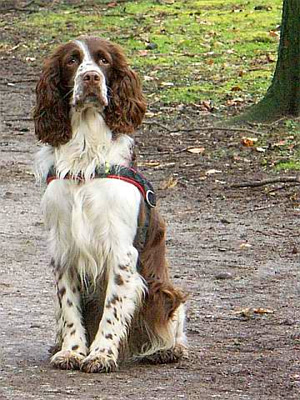
\includegraphics[height=4cm]{spaniel.jpg}
\includegraphics[height=4cm]{wolf.jpg}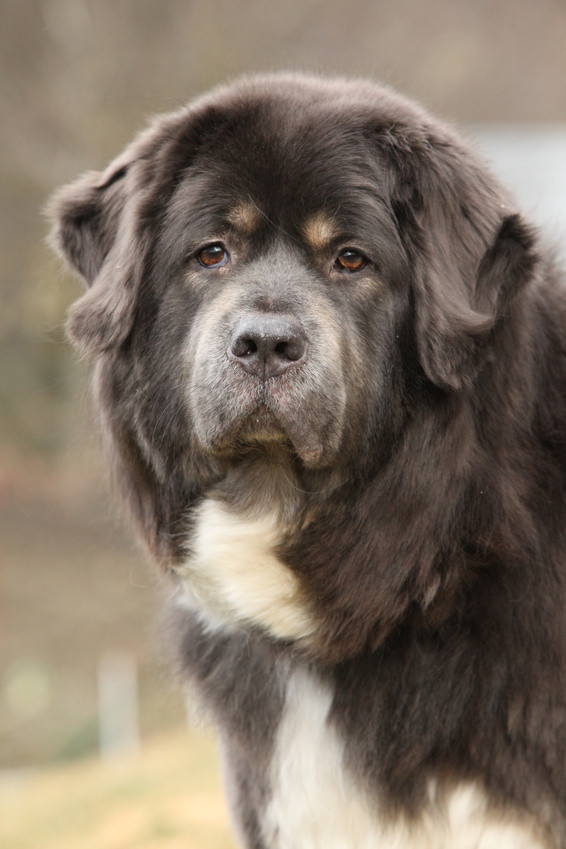
\includegraphics[height=4cm]{mastiff.jpg}
		\caption{Spanjel, hunt ja mastif}
	\end{center}
\end{figure}

Niisiis, koodi ümber kirjutamine on kallis, keeruline ning seotud oluliste riskidega. Samas on olemasoleva rakenduse putitamisel samuti üks oluline puudus: me toimime jätkuvalt kord juba defineeritud arhitektuuri, täpsemalt öeldes kontseptsiooni, raamides. Ehk, asjade ümber kirjutamine annab võimaluse innovatsiooniks ning asjade puhtalt lehelt uuesti mõtestamiseks. Jah, spanjelist on ilmselt võimalik mastifi-laadne elukas aretada aga võibolla on efektiivsem alustada siiski nende ühisest eellasest, hundist? Kindlasti tuleks keskenduda mitte tehnilisele vaid ärilisele innovatsioonile ümber mõtestades äriprotsesse, automatiseerides ning efektiivistades. Seejuures on muidugi eelduseks, et meil on piisavalt aega ja raha seda mõttetööd põhjalikult ette võtta ning et on alust eeldada, et tulemus praegusest olukorrast oluliselt erineb.

Lõpuks tuleb panna kõrvuti süsteemi ümber kirjutamise kulu, olemasoleva muutmise ning mõlema alternatiivi halduskulude nüüdisväärtus. Kui nüüd tundub, et rakenduse uuesti kirjutamine on siiski mõistlik, on oluline aru saada, miks nii läks. Jällegi Joelile toetudes, ei ole mõistlik eeldada, et kui ühel korral ei õnnestunud hankida mõistlikku süsteemi või seda pusaks muutumast hoida, siis teisel korral asjad teisiti lähevad. On oluline, et suudetakse välja tuua konkreetsed tegevused, mille abil hoidutakse vajadusest süsteem uuesti ümber kirjutada. Siinkohal kuuleb ilmselt argumenti \emph{build one to throw away} aga sel juhul peaks olema võimalik vähemalt üles kirjutada, mida esimesest korrast täpselt õpiti.

\TODO:  \cite{nlp}, kontseptsiooni venitamise idee. Kui nii funktsioon kui vorm on arenenud kaugemale algsest kontseptsioonist.

\subsection{Taakvara ja testid}
Taakvara\index{Taakvara} võib määratleda ka tarkvaratehnilisest küljest. \citeauthor{feathers2004working} määratleb taakvara kui lihtsalt testideta koodi. \cite{feathers2004working} Ta arutleb nii: kui koodil ei ole teste, ei saa me teda muuta. Ükskõik kui hästi, puhtalt ja kenasti kood ka kirjutatud ei ole, ei tea me tema käitumisest ilma testideta midagi. Veelgi enam, me ei tea midagi tema \emph{olulisest} käitumisest. Kood võib toimida väga erinevatel viisidel aga ilma testideta ei ole meil võimalik eristada soovitud käitumist soovimatust. Ja kui nii, siis ei ole ilma testideta võimalik hinnata, kas meie kood läheb muutuste järel paremaks või halvemaks. Nii on aga sihipärane koodi muutmine võimatu.

Kui aga koodi muuta ei saa, muutub ta varast kohustuseks. Nii ei ole testimispõhine taakvara definitsioon mitte nii ärikauge, kui algselt paistab: argumentatsiooni juured on ärilise väärtuse\index{Väärtus} lisamises.

\section{Tehniline võlg}
\index{Tehniline võlg}
On kriitiline, et tellija\index{Tellija} saaks aru oma tegevuse tagajärgedest. Mis, arvestades teo ja selle tagajärje ajalist vahet, on väga keeruline. Põhjus on selles, et tehnilise võla likvideerimine tuleb arenduse läbilaskevõime arvelt. Järelikult tähendab tehnilise võla kuhjumine, et arenduse läbilaskevõime ajas kahaneb. Kui tellija ei saa aru, et tema otsus tekitas tehnilise võla, on IT-juhil kaks põhimõttelist otsust. Ta kas keeldub tehnilist võlga tekitamast, näib paindumatu ja lastakse lahti või ta võtab tehnilise võla, asub seda IT võimekust vähendades likvideerima ning ta lastakse lahti. Ehk, häid valikuid ei ole. Järelikult ei ole IT juhil muud valikut peale tellija harimise.

Tehnilise võla oluline aspekt on seotud süsteemi piiride küsimusega. Kuna tehniline võlg on seotud konkreetse süsteemiga kuid, definitsiooni järgi, on süsteemi piirid alati suvalised, võib rääkida tehnilise võla skoobist. On võimalik olukord, kus lokaalsete optimumide saavutamise läbi võetakse süsteemi kui terviku suhtes tehnilist võlga. Näiteks võib ehitada kõik süsteemid tähtajaks kuid mitte arvestades teiste süsteemi osade integratsioonivajadusi. Üksiku süsteemi vaatepunktist võlga ei ole. Süsteem kui tervik aga võib vajada olulist investeeringut oma komponentide suhtluse tagamiseks. 

Tehnilise võla juhtimine on teatavas mõttes sarnane finantsvõla juhtimisega: rahavoogude nüüdisväärtuse abil on võimalik teha otsuseid. Tehnilisel võlal on siiski ka aspekte, mida lihtsasti finantsmudelisse valada ei õnnestu. Teatavast piirist alates hakkab tehniline võlg takistama värbamist ja inimeste hoidmist. Tegemist on raskestivarjatava stressifaktoriga ning üha vähem leidub inimesi, kes \enquote{selle supiga} on nõus tegelema. Nii võib alata lõigus \ref{sec:kokkuhoid} kirjeldatuga sarnane tagasiside, kus kompetentsete inimeste lahkumine viib võla suurenemiseni mis omakorda tõrjub kompetentseid inimesi. 

\section{Tehnilise võla teine külg}
Võlal on alati kaks poolt. Saab võlgu anda ja saab võlgu võtta. Kas tehnilise võlaga on ka nii? Selle koha peal, kardetavasti, saab meie metafoor otsa. Sest päris täpset vastet võla andmisele ei ole. Küll aga võime endale tuleviku ees kohustusi võtta mitte tööd tegemata jättes vaid seda liiga palju tehes\sidenote{Siin suurepärased näited: \url{http://hackingdistributed.com/2016/04/05/how-software-gets-bloated/}}. 

Olgu meil tegu süsteemiga, mis on suur, keeruline ja raskesti muudetav. Sellega toimetavad nutikad ja hästi makstud inimesed. Nutikad ja hästi makstud inimesed suudavad lahendada keerulisi probleeme, seepärast nad hästi makstud ongi. Aga paraku on nutikatel inimestel komme mõnikord ka lihtsaid probleeme natuke keeruliselt lahendada. Ja isegi, kui probleem tõepoolest keerulist lahendust õigustab, tekib küsimus: kas me suudame edaspidi leida piisavalt nutikaid inimesi? Ja kui suudame, siis kas on inimlikult võimalik keeruliste lahenduste kohta käivat teadmust mõistlike kadudega ühest peast teise liigutada? 

Skype kui selline on hea näide sedalaadi keerulisest süsteemist. P2P\index{Skype!P2P} võrk on ülikeeruline ja väga elegantne lahendus keerulisele ärilisele probleemile. Lahenduse hind oli aga, et ainult väike hulk väga häid programmeerijaid suutis tolle võrgu arendamisega tegeleda või isegi sealseid probleeme hoomata. Mõelge näiteks algoritmile, mis suudab paarikümne osalejaga sõnumi-vestluste olekut\sidenote{Sealhulgas nii sõnumid kui ka näiteks lisatud ja eemaldatud osalised. Sõnumeid kirjutada, kasutajaid lisada ja eemaldada jne. on võimalik ka ilma võrguühenduseta. Tegu on ühe eriti keerulist liiki konsensusprotokolliga.} kõigi osapoolte vahel sünkroniseerida. Selle algoritmi kohta oli peamine teadmine ühe inimese peas ning kui too põhjalikku dokumentatsiooni maha jättes lahkus, ei õnnestunudki kogu teadmist üle võtta.

Üks arhitektuuri puhul kehtivatest printsiipidest on, et süsteemi disain ei tohi eeldada kõrgemat tootmisvõimekust, kui planeeritud. Disainides F1 stiilis tolerantsidega mootori ja andes selle toota tavasõidukite mootorite tehasele, ei saa tulemus hea olla. Väga paljud infosüsteemide hädad tulenevad liiga headest arhitektidest, kes loovad efektseid keerulisi süsteeme arvestamata, et neid hakkavad realiseerima täiesti keskmised tavalised programmeerijad. 

Keerukuse kasvu ei saa paraku alati arhitektuursete vahenditega vältida. Programmeerijale jääb reeglina mingi vastutus disainiotsuste üle ja seal võib kergesti olla ruumi äärmiselt keerulistele lahendustele. Kerkinud keerukuse-probleemi lahendamine on reeglina siiski arhitekti ülesanne. 

Jõuame olulise järelduseni, et nii arhitekti töö kui süsteemi jätkusuutlikkus tervikuna sõltuvad mitte ainult kasutatavate programmeerijate kompetentsist vaid ka organisatsiooni võimest seda kompetentsi taset hoida või kasvatada. Järelikult on arhitekti starteegiline huvi mõista asutuse personali- ja koolituspoliitikat.Kui see ebasoovitavas suunas muutuma peaks, tuleb otsustajaid riskidest teavitada kuid kindlasti ka omalt poolt maandamismeetmeid tarvitusele võtta.


\section{Alandlik programmeerija}
\label{humble}
Edsger W. Dijkstra\index{Dijkstra, Edsger W.} on inimene, kes arvuti-inimeste hulgas tutvustamist ei vaja ja kel tiitleid rohkem, kui loetleda jõuab. Muu hulgas on ta 1972. aastal saanud Turingi Auhinna. Nagu kombeks, järgnes auhinnale avalik loeng \citep{yourdon1979classics}, mille pealkirjaks Alandlik Programmeerija. Pika ja tõeliseks nautimiseks mõningast arvutiteaduse tausta vajava jutu peamised teesid on järgmised\footnote{Tõlgitud ja mugandatud aadressilt \url{http://c2.com/cgi/wiki?TheHumbleProgrammer}}:
\begin{itemize}
	\item Kui pürgida töökindla tarkvara ja efektiivse töökorralduse poole, peate leidma viisi vigade vältimiseks nende hilisema otsimise asemel. Selle tulemusena muutub programmeerimine kui protsess odavamaks.
	\item Programmeerijad peaksid tegelema vaid intellektuaalselt hoomatava tarkvaraga
	\item Programmeerijad ei peaks unustama, et nende ülesanne ei ole programmeerida. Nende ülesanne on disainida lahendusi, mis käituvad soovitud viisil
	\item Tavaliselt kirjutatakse programm ja siis seda testitakse. Kuid testimine on paremal juhul efektiivne viis vigade olemasolu tuvastamiseks. Vigade puudumise  tõestamiseks on testimine lootusetu
	\item Kompetentne programmeerija on teadlik oma pea väga piiratud suurusest. Seega läheneb ta programmeerimisülesandele alandlikus meeles ning, muu hulgas, väldib nutikaid trikke nagu katku
	\item Kohmakas tarkvaratehnika on talutav vaid senikaua, kuni riistvara moodustab suurema osa projekti eelarvest
\end{itemize}

\section{Küsimusi aruteluks}
\subsection{Mis teeb programmeerimise keeruliseks?}

Brooks\index{Brooks, Frederick P.} ütleb, et programmeerimine on põhimõtteliselt keeruline\cite{brooks1975mythical}. Ta jagab tarkvaratehnilise keerukuse kaheks, mitteolemuslikuks ja olemuslikuks, ning väidab, et neist esimene on vähendatav ja teine tõenäoliselt mitte. Olemuslik keerukus seisneb peamiselt tarkvara kontseptuaalse mudeli spetsifitseerimises, disainis ja testimises ja mitteolemuslik tolle mudeli võimalikult täpses koodi valamises. 

Kuid Brooks ei seleta väga põhjalikult \emph{miks} töö tarkvara kontseptuaalse mudeliga (mis on sisuliselt seesama, mida me eespool süsteemi kontseptsiooniks nimetasime) põhimõtteliselt keeruline on. Tõenäoliselt on vähemalt üks põhjus arvutite duaalses olemuses. Kogu tänapäevane digitaalne arvutustehnika on üles ehitatud kahevalentsele loogikale. Null ja üks, tõsi ja vale. Täidetakse kas üks koodi haru või teine. Samas pole reaalne maailm sugugi duaalne. Ei leidu ei puhast musta ega valget. Loodus ei tekita ei päris ümmargusi ega päris kandilisi objekte. Ja nii peabki programmeerija suutma konstrueerida mudeli mis ühest küljest peegeldab reaalsuses toimivat ja sellisena ebatäiuslikku äriprotsessi ja teisalt on realiseeritav digitaalarvutiga. Selline tegevus ei ole olemuslikult lineaarne ja tõenäoliselt praeguses tarkvaratehnika paradigmas hästi automatiseeritav ei ole. 

\begin{marginfigure}
		\begin{center}
		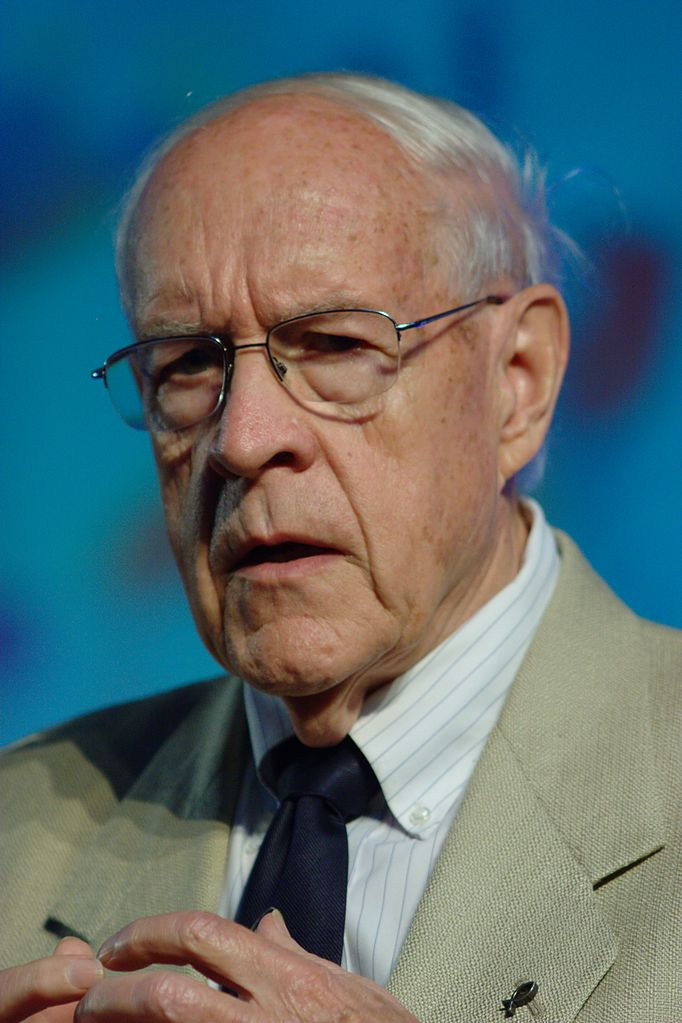
\includegraphics[width=.7\linewidth]{682px-Frederick_Brooks_IMG_2279.jpg}
		\caption{Fred Brooks. Pilt: wikimedia:user:David.Monniaux}
		\label{fig:brooks}
		\end{center}
		Fred Brooks on legendaarne arvutitegelane, kes juhtis IBM\index{IBM} System/360 ja OS/360 arendust. Saadud kogemusest kirjutas ta oma põhiteose, The Mythical Man-Month ning oli hiljem tegev arvutiteadlasena. 
\end{marginfigure}

Kui miski on keeruline, tekitab see kulusid. Kui miski tekitab kulusid, siis on võimalik müüa vahendeid tolle miski vähendamiseks. Ja kuna olemusliku ja mitteolemusliku eristamine mitte lihtne ei ole, siis on läbi ajaloo üritatud üle saada ka tarkvara ehitamise keerukuse probleemist:

\begin{description}
	\item[Nõuete kirjeldamine] Kui me ainult suudaksime nõudeid piisavalt täpselt kirjeldada (ehk oma maailmamudeli võimalikult täpseks ajada), siis on seda võimalik ka üheselt tarkvaras realiseerida. Täna ei leidu vast praktikut, kes sellise väitega nõus oleks. Siiski panustavad mõned metoodikad siiani nõuete ülitäpsesse kirjeldamisse. Mudeli lahutuse tõstmine viib järjest uute detailide esilekerkimiseni mis paratamtult omakorda paljastavad uusi detaile. Kas laud on sile näpuga katsudes, molekuli, aatomi või elektroni tasemel? Äkki peaks rääkima hoopis väljavõrranditest?
	\item[Protsessi järgimine] Kui me ainult suudaksime välja mõelda deterministliku tarkvara loomise protsessi ja panna kõik osapooled seda järgima, peab tulemus olema deterministlik. Paraku ei ole ka parim lineaarne protsess täielik mittelineaarse tegevuse lähend. Nagu ka nõuete juures ilmneb ka parima protsessi puhul järjest uusi nüansse, mida protsessis arvesse võttes paljastub järgmine kiht keerukust
	\item[Artefaktide tootmine] Kui me ainult suudaksime määratleda iga tegevuse täpse tulemi ja sisendi, võiks neid tegevusi vabalt kombineerides saada vähemalt täieliku pildi projektis toimuvast. Ka see tee ei vii suurt kuhugi. Järjest täpsem loova inimese peas toimuva kirjeldamine võtab järjest rohkem aega, viies projekti hilinemiseni, mida ma ju teadupärast lahendame järjest rohkemate ja detailsemalt määratletud artefaktide nõudmise abil
	\item[Protsessist loobumine] Kui me oleme kõike eeltoodut juba proovinud, siis kui me vaid suudaksime kogu selle massi alt programmeerija üles leida ja vabastada, siis hakkaksid ju projektid kohe paremini välja tulema? Selles mõtteviisis on agiilsete meetodite juured. Paraku tavaliselt selgub peagi, et ilma protsessita toimetamine nõuab palju suuremat distsipliini, kui protsessiga ning piiravaks teguriks saab inimeste võimekus omavahel abstraktseid ideid jagada. 
\end{description}

Kõiki neid lahendusi on eri aegadel müüdud kui lahendust tarkvara keerukusele ning ilmsel toob tulevik uusi sedalaadseid. Kuid kuni inimene koodi kirjutab, on ja jääb tarkvara tegemine keeruliseks ning mao-õli müüjatesse tasub suhtuda skepsisega.

\subsection{Kuidas seletada juhtkonnale tehnilist võlga?}
Oma otsuste (eeldades, et võlg on võetud ärilistel põhjustel) tagajärgedega silmtsi seismine ei ole kunagi lihtne\sidenote{Osalt on sellest küsimusest juba eelnevalt räägitud, vt. \nameref{sec:business:q1}}. Põhimõtteliselt on probleem selles, et isegi suhteliselt lihtsa dünaamilise mudeli käitumine ei ole intuitiivne ning lihtsasti mõistetav. \citeauthor{ledet1994manufacturing} on tegelenud keeruliste dünaamiliste mudelitega tootmisettevõtetes\cite{ledet1994manufacturing}. Nad leidsid, et probleemi tuvastamine arvutimudelite abil on suhteliselt lihtne kuid tulemuse presenteerimine viisil, mis ka organisatsioonilise muutuse esile kutsuks, on keerukas. Nad proovisid kolme lähenemisviisi.

Esmalt üritasid nad seletada mudelit, selle eeldusi ning näidata tulemusi. Tulemus oli pettumustvalmistav. Kuna mudeli tulemus on reeglina suhteliselt triviaalne, tekkis tihti küsimus \enquote{kas tõesti pidi mudel teile seda ütlema?} ning eelduste selgitamine oli kõigile osapooltele frustreeriv.

Teiseks presenteeriti mudeli tulemusi seletamata nende saamise viisi. Tegu oli küllalt efektiivse lähenemisega, mille tulemused kergesti omaks võeti. Kuna, jällegi, mudeli tulemus on triviaalne kostis tihti kommentaare stiilis \enquote{ma olen seda juba aastaid rääkinud!}.\sidenote{Tekib siiski küsimus, kust ja miks said analüütikud nende tõsiselt võtmiseks piisava usalduskrediidi}

Kolmandaks loodi simulatsioonimäng ja mängiti see multidistsiplinaarse meeskonnaga ka läbi. Nii oli osalistel võimalik mitte ainult modelleerimise tulemust näha vaid selleni ka iseseisvalt ja ohutus keskkonnas jõuda. 

Sarnaste tulemusteni on jõutud ka mujal. MIT Sloan School of Management uurijad arendasid kuuekümnendatel välja \enquote{õllemängu}\cite{sterman1984instructions}. Mängu mõte on demonstreerida osalistele ka lihtsate tarneahelate kõrget dünaamilist keerukust ning võimaldada kasutada erinevaid sellega toime tuleku strateegiaid. Mängus osalejad simuleerivad poest, hulgimüüjast ja tootjast koosnevat õlle tarneahelat, kus iga sammu vahel on ajaline nihe. Tuleb välja, et ka mõne käigu kaugusele ulatuv vahe põhjuse ja tagajärje vahel ei ole lihtsasti hoomatav ning osapooled kipuvad kergesti pankrotti minema. Seda ka pärast põhjalikku mängu ja tema olemusega tutvumist. 

Ehk, tulles tagasi algse probleemipüstituse juurde, ei ole juhkonnale tehnilise võla selgitamine lihtne ülesanne. Enamasti ei ole IT juhi kästuses ei mänguvõimalust ega ka modellerimisvõimekust. Mida tavaliselt siiski teha õnnestub, on tehnilise võla läbipaistvaks muutmine näiteks arendussaba\index{Arendussaba} nähtavaks muutmise läbi. Seda saab omakorda teha tavalise veahaldustarkvara abil. Oluline on silmas pidada, et too saba siis ka tõesti soetud oleks ning sisaldaks igal hetkel selgelt markeerituna asju, mida on eksplitsiitselt otsustatud mitte teha. 

\chapter{IT valitsemine}
\section{Parimatest praktikatest}
\label{sec:governance:bp}
IT valdkonnas on käibel suur hulk kõivõimalikke metoodikaid ja raamistikke. Osa neist on ühel või teisel viisil kogumid parimatest praktikatest: grupp ettevõtteid on kokku leppinud, et mingisugune konkreetne viis mingisugust konkreetset probleemi lahendada on parim. Sellised on näiteks ITIL\index{ITIL} ja TOGAF\index{TOGAF} aga ka PMBOK\index{PMBOK}. Teataval määral on ka käesolev kogumik - kuigi tugineb vaid ühele inimesele - samast puust. 

Kindlasti on parimatel praktikatel oma väärtus, tegemist on ju õitsva äriga. ITIL annab väga hea ülevaate erinevatest IT juhtimisega seotud valdkondadest, PMBOK teeb sama projektijuhtimisega. Samas tuleb neisse suhtuda teatava ettevaatusega. Asi on selles, et parim praktika on tahes tahtmata keskmine. Leitakse hulk viise probleemi lahendada ning mõõdetakse nende edukust. Raamistikku jõuab miski, mis on nii laialt levinud kui edukas. Kuid organisatsioon, mis järgib keskmisi praktikaid saab paratamatult olla vaid keskmine. Samuti ei tähenda mõne praktika populaarsust, et tegemist on \emph{parima} praktikaga\sidenote{\quote{If majority is always right - let's eat shit... millions of flies can't be wrong.}\\Waldemar Łysiak}. Tegu on vaid parima teadaoleva praktikaga valimis. Kui suur hurk turuosalisi teeb näiteks konfiguratsioonjuhtimist ühel viisil, siis ei saa konfiguratsioonijuhtimine pakkuda ühele neist võimalust eristuda. 

Veelgi enam, seda keskmist ei olegi olemas\cite{averages}. On hulk organisatsioone, mis järgivad \emph{igaüht} neist praktikatest kuid ei ole organisatsiooni, mis järgib neist \emph{kõiki}. Ei ole mõistlik üritada olla nagu teised, sest, paradoksaalselt, mitte keegi ei ole selline nagu teised. Tuleks üritada leida lahendus oma probleemile ning määratleda just konkreetsele organisatsioonile sobiv tasakaal standardsete strateegiliste eeliste vahel.

Loomulikult on hulk valdkondi, kus eristuma ei peagi, mille kallal pea murdmine ei loo piisavalt väärtust. Kuid tänapäeval on üha väiksem hulk neist infotehnoloogias sest efektiivset eristumisvõijust otsitakse järjest enam just ITst.

\section{Poliitikavastasus. Hundid ja jänesed}
\index{Poliitikavastasus}

Kujutlegem lihtsat ökosüsteemi, mis koosneb huntidest ja jänestest. Hundid söövad jäneseid, jänesed elavad õhust ja armastusest (mida mõlemat on piisavalt). Loomade omavahelisi seoseid illustreerib joonis \ref{fig:wolves}. Oletagem, et meil on soov tõsta huntide arvukust. Seepärast tuuakse mujalt ja lastakse metsa lahti viis emast ja viis isast hunti. Mis juhtub? 
\begin{itemize}
	\item Huntide arvukus tõuseb kümne lisandunud hundi võrra
	\item Kuna kümme lisandunud hunti tahavad süüa, siis väheneb jäneste arvukus. Ajaühikus ära söödavate jäneste hulk ju suureneb
	\item Kuna jäneseid on vähem, väheneb ka jäneste juurdekasvu kiirus. Ära söödud jänesed ju uusi jäneseid ei tee. Samuti tahavad uued hundid ka homme süüa
	\item Seega hakkab jäneste arvukus vähenema
	\item Misjärel hakkavad hundid nälga jääma, sest kõigile enam jäneseid ei jagu
	\item Mistõttu saavad hundid vähem järglasi ja langeb nende juurdekasvu kiirus
	\item Kuna hundid surevad vanadusse ikka sama tempoga, hakkab huntide arvukus vähenema
	\item Kui huntide arvukus on jõudnud esialgsele tasemele, on kõigile jälle piisavalt jäneseid 
\end{itemize}

\begin{marginfigure}
		\begin{center}
		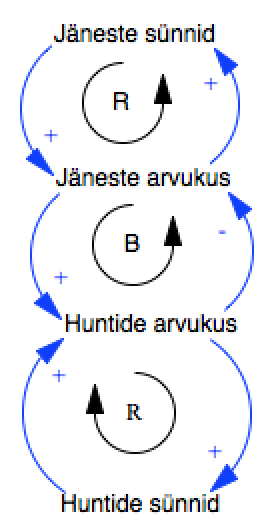
\includegraphics[width=.7\linewidth]{hundid.png}
		\caption{Huntide ja jäneste arvukuse seos}
		\label{fig:wolves}
		\end{center}
	Huntide ja jäneste arvukuse seos. Nii huntide kui jäneste puhul viib rohkem loomi rohkemate sündide ja seega rohkemate loomadeni. Kuid huntide arvukuse kasv viib alla jäneste arvukuse ning jäneste arvukuse langus viib alla huntide arvukuse.
\end{marginfigure}

Nii taastub esialgne olukord, algne huntide lisamine ei ole andnud soovitud tulemust. Huntide arvukus võiks tõusta hoopis tõstes jäneselaste arvu jäneseperekonnas ehk nende juurdekasvu kiiruse tõstmisega. 

\section{Inimeste valitsemine}
Valitsemise üsna lahutamatu osa on paraku vajadus inimesed organisatsioonist eemaldada. Jättes kõrvale juriidilised ja muud nüansid, on oluline aru saada, et mõtteliidri (\emph{thought leader}) lahkumine on meeskonna dünaamika jaoks oluline sündmus. Samuti on oluline mõista, et tegu on vältimatu protsessiga, mis seega on mõistlik läbi viia kontrollitult ja minimaalsete kadudega. Järgnevas selleks mõned näpunäited: 

\begin{itemize}
	\item Vii inimene organisatsioonist välja enne, kui tema vastuolud muutuvad meeskonna vastuoluks. Definistiooni järgi inimesed järgnevad liidrile ning kui tollel on kellegagi vastuolud, kanduvad nood paratamatult varem või hiljem meeskonda. Kui hiljaks jääda lahkuvad (või tuleb vastuseisu tõttu eemaldada) ka teised tiimi liikmed peale juhi. Nii võib oskamatu käitumisega vallandada lumepalliefekti, mis organisatsiooni kiiresti ajudest tühjendab.
	\item Väike (!) hulk võtmeisikuid peab plaanist ette teadma, sealhulgas muidugi ka eemaldatav ise. Nii on neil ühest küljest võimalik tulevaseks kriisiks valmistuda kuid teisalt saab nii vältida emotsionaalset avalikku käitumist ning muidu üllatusi. Etteteatamisaeg võib ulatuda mõnest päevast mõne tunnini. Pikem aeg tekitab permanentse kriisi olukorra ja kommunikatsioon väljub kontrolli alt
	\item Kommunikatsiooni kolm sammu. Kõik sammud läbitakse väga lühikeste (kõige rohkem mõned tunnid) intervallidega vältimaks uudiste lekkimist (ingl. \emph{techcrunch meltdown} tuntud tehnoloogiauudiste portalli järgi) ning minimeerimaks kriisi kestvust. 
		\begin{enumerate}
			\item "Vanaisa"\footnote{Juhi juht. Selles kontekstis isik, kes teeb otsuse inimene välja viia.} teade. Nii antakse teada, kes olukorda kontrollib. Sisaldab
				\begin{itemize}
					\item Kes lahkub millal ja miks. Tekst olgu viisakas, inimesed kas teavad niigi või suudavad ridade vahelt lugeda
					\item Mis juhtub järgmisena ja millal. Inimestele ei meeldi ebakindlus, hirmud tuleb maha võtta. Oluline punkt siin: kes ja millal asendab lahkuja?
					\item Muutused organisatsiooni toimimises. Lahkuja oli kindlasti osaline mingites äriprotsessides (koodi ülevaatused, tarnete vastu võtmine jms.), kuidas need edasi toimima hakkavad?
				\end{itemize}
			\item Lahkuja teade. Tavaliselt suunatud lähematele kolleegidele. Võib olla suhteliselt otsekohene aga kui on karta midagi mürgist, võib (viisakalt) paluda teksti kooskõlastamist
			\item Avalik teade. Kui vähegi usutav, võiks tekst olla kiitvas, positiivses ja tänulikus toonis. Kui mitte, siis lakooniline kuiv tekst.
		\end{enumerate}
\end{itemize}

\section{Ressursijuhtimine}
Järgnev on üks võimalik vaade asjadele: selgesti on avaliku- ja erasektori suhtumine rahasse erinev. Ainus põhjus, miks maksumaksja riigile raha annab, on, et selle raha eest osutataks avalikku teenust. Kui nüüd riik korjab raha kokku, kuid selle eest mõistlikku avalikku teenust ei osuta (ka reservide kogumine on avalik teenus), siis on tegu maksumaksja asjatu koormamisega. Erasektoris jaotatakse kasum omanike vahel, riigis selle mehhanismi ekvivalenti ei eksisteeri. Järelikult on erasektoris pigem surve raha mitte kulutada samas kui riigisektoris on pigem surve raha eest võimalikult palju teenust osutada.  

\section{Surnumere efekt}
Miks on Surnumeri soolane? Põhjus on lihtne: sinna lisandub küll suhteliselt soolast vett aga füüsikaseaduste tõttu aurab ära  vaid puhas $H_2O$. Nii võib kergesti juhtuda ka organisatsioonidega\sidenote{Loe lähemalt \url{http://brucefwebster.com/2008/04/11/the-wetware-crisis-the-dead-sea-effect/}}, eriti IT omadega. Lühidalt öeldes, organisatsiooni sisenevate ja sealt väljuvate inimeste talendi, hariduse, suhtumise, kogemuse ja oskuste tase ei lange kokku. Värvata õnnestub tõenäoliselt suhteliselt normaaljaotuse lähedast kontingenti kuid lahkuvad reeglina paremad. Ja nii tekib tagasiside: mida hullem on olukord organisatsioonis, seda nõrgemaid kandidaate õnnestub värvata, seda kiiremini filtreeruvad välja halvimatest parimad ja seda hullem on olukord. 

Kuidas tsükkel tekib ning kuidas sellest vabaneda? Tegu on olemuselt juhtimisprobleemiga. Kui vesi soolaseks läheb, on keegi on kuskil teinud juhtimisvea. Kuid käivitajaks võib olla ka viga personalitöös\index{Personal}. Näiteks võib kiire laienemise käigus organisatsiooni sisse tulla olemasolevatest oluliselt nõrgemaid inimesi või on kasutusel ebakompetentsuse suhtes tolerantne hindamissüsteem. Kuidas ka ei oleks, on oluline pidada silmas nii tulijate kui lahkujate oskusi. Kui me kaotame rohkem nutikaid inimesi (näiteks tiheda turusituatsiooni tõttu), peame ka palkamise sinnapoole kallutama. Vatupidine olukord - kaotame pigem keskmisest vähemnutikaid - võib tunduda isegi soovitavana kuid ka siin on omad ohud. Vaid staaridest koosnevad meeskonna koos hoidmine nõuab oluliselt kõrgemat juhtimiskompetentsi ning kindlasti tuleb silmas pidada ka palgataseme mõju ärimudelile.

Eriti sagedasti võib surnumere laadset mõistuslikku elu mitte toetavat keskkonda leida riigiasutuste IT-osakondades. IT organisatsioonid on efektile suhteliselt vastuvõtlikumad, kuna seal on isikliku panuse ja tulemuse seos tugev, tööjõuturgu teeb pakkuja ning inimeste omavahelised suhted on tihedad. Teisalt on riigiasutuses tavaliselt suhteliselt jäigad personaliga seotud reeglid, mis teevad inimestest organisatsiooni initsitatiivil vabanemise keeruliseks. 

\section{Protsesside juhtimine}
\subsection{Organisatsiooni kiirendamine}
Suurepärane näide organisatsiooni kiirendamisest on Singapur. Joonisel \ref{fig:kasv} on toodud viie riigi GNI aastatel 1995 kuni 2012. On näha, kuidas USA, Eesti, Läti ja Vene Föderatsioon kasvavavad suuresti samas rütmis, kuigi absoluutnumbrites on USA teistest kaugel ees. Singapur aga on suutnud aastast 2002 näidata teistest oluliselt kiiremat kasvu. Isegi arvestades 2008. aasta kriisi mõju, on kasv teistest oluliselt kiirem. Lühike järeldus joonisest on, et ühel või teisel viisil on Singapur suutnud mitte ainult kasvada, vaid kasvada teistest kiiremini. Kui Eesti aga ka jätkab senist stabiilset kasvu, ei õnnestu meil ilmselt kunagi USAle järele jõuda. 

\begin{figure}[h]
	\begin{center}
		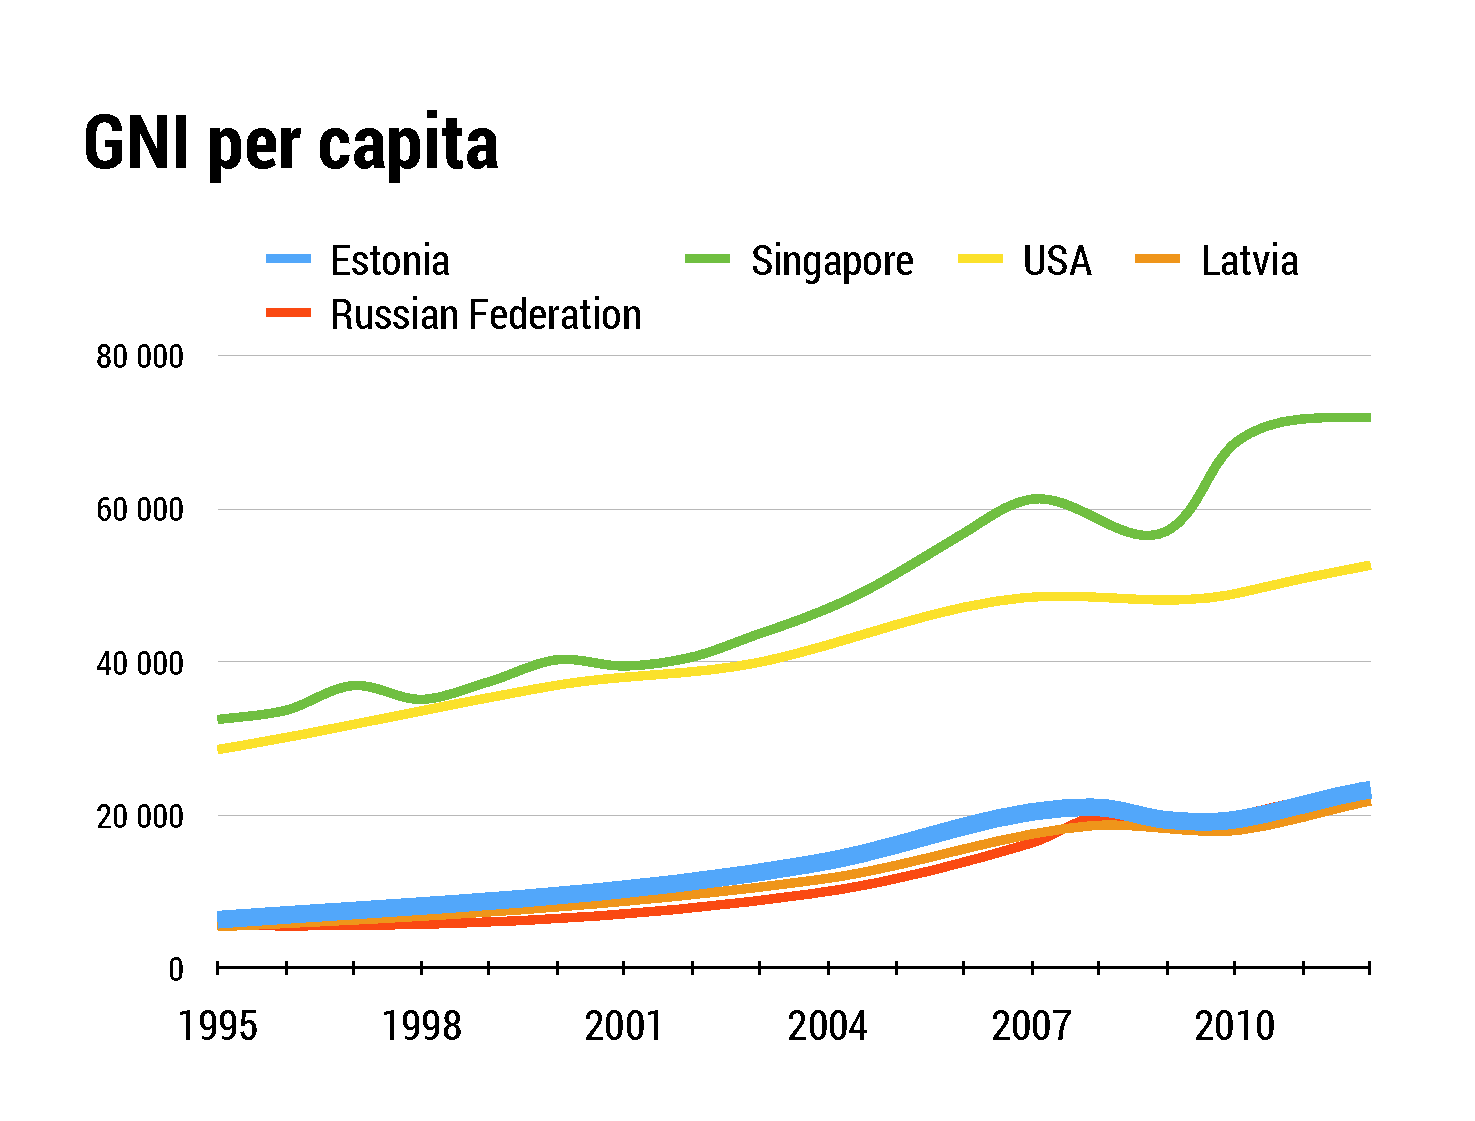
\includegraphics[width=\textwidth]{kasv.pdf}
		\caption{Riikide GNI võrdlus. Maailmapanga andmed.}
		\label{fig:kasv}
	\end{center}
\end{figure}

\subsection{Arenduse ootejärjekorra juhtimine}
Infotehnoloogia on tavaliselt põimunud sügavale organisatsiooni protsessidesse. Samuti on IT peamine protsesside efektiivistamise vahend. Järelikult on igas organisatsioonis suur hulk erinevaid arendusvajadusi. Samas on ressursid alati piiratud\footnote{Rangelt võttes võib probleemiks olla ka võimekus ressursside omavaheline vahetus. Näiteks on suurettevõtetes või avalikus sektoris tihti piiratud täistööajaga töötajate hulk, samuti võib saadaolev finantseering olla seotud pirangutega (selle kulutamine teatud riigis või teatud tegevusteks)} ning seega ületab organisatsiooni arendusvajadus reeglina IT-organisatsiooni võimekust seda vajadust täita\footnote{Vt. ka lõik \ref{sec:kulud} organisatsiooni võimekuse arengu kohta}. Järelikult kerkib küsimus tööülesannete järjestamisest. Mis järjekorras töid ette võtta?

Ootejärjekorral on järgnevad omadused:
\begin{itemize}
	\item Kuna töid tekib definitsiooni järgi kiiremini, kui neid täita suudetakse, siis järjekord kasvab. Kui vannist voolab vesi aeglasemalt, kui seda sinna lisandub, hakkab vee tase tõusma
	\item Mida pikem on ootejärjekord, seda paindumatum on organisatsioon. Kui järjekorras on x aasta jagu projekte, siis jõuab järjekorra viimane tegemisse kõige kiiremini x aastaga
	\item Kuna organisatsiooni äritulemuste saavutamine sõltub sageli ITst, eksisteerib ootejärjekorrale tugev poliitiline surve. Otsus mõnda projekti teha ja teist mitte võib omada mõne osalise jaoks omada isiklikku väljundit tulemustasu näol
\end{itemize}

Et ootejärjekord on pikk, tuleb ühel või teisel viisil sealt kas projekte välja jätta või vähendada organisatsiooni võimekust sinna asju lisada. Et otsused on seotud konfliktiga, minnakse sageli just ootejärjekorra barjääri tõstmise teed. Oma rolli mängib siin ka soov olemasolevat võimalikult efektiivselt kasutada suunates klienti võimalikult põhjalikku eeltööd tegema. IT kliendiks oleva keskastme juhi vaatenurgast vaadates tekib nii olukord, kus tema (organisatsiooni perspektiivist väheoluline, kuid tema jaoks kriitiline) arendusvajadus vajab ebaproportsionaalselt palju panust ning omab ikkagi väikest shanssi töösse minna. Eriti drastiline on probleem harukontorite puhul, millede probleemistikust ei pruugi lõpuni aru saada ka peakontori inimesed. Kui nüüd tollel juhil on initsiatiivi, juhtub tavaliselt üks kahest. Kui käepärast on krediitkaart, siis võidakse probleemi lahendamiseks hankida marginaalse hinna eest teenust mõnelt SaaS\footnote{\emph{Software as a Service} tarkvara kui teenus. Lahendus, kus tarkvara hallatakse keskselt ning lõppkasutaja maksab teenuse eest perioodiliselt proportsionaalselt teenuse kasutamisega} pakkujalt. Mispuhul tekib reeglina kohe riskijuhtimislik probleem sest kaob kontroll organisatsiooni andmete üle. Kui aga käepärast on IT-kompetentsi kas Exceli makrode või PHP tundja näol, luuakse tõenäoliselt kohalik infosüsteem. Sedalaadi infosüsteem ei vasta tavaliselt ühelegi keskse IT standardile, muutub ühel hetkel tellija jaoks kriitiliseks, kaotab oma ainsa arendaja (vahel kõike korraga) ning paneb keskse IT fakti ette: üle tuleb võtta dokumenteerimata, ebaturvaline ja profiilist välja jääv ärikriitiline tehniline lahendus. Tekitatud pusa ümber kirjutamiseks (kui isegi leidub keegi, kes suudaks sellise ülesande pädevalt püstitada) reeglina finantseeringut leida ei õnnestu. 

Taoliste olukordade vältimiseks on kriitiline, et järjekorrast projektide välja jäätmine oleks põhjalikult dokumenteeritud kui \enquote{sellega-me-ei-tegele-siin-majas} otsus ning et eksisteeriks ülevaade barjääri taga toimuvast. Samuti võib soovitada eraldi protsessi väikesemahulisteks arendusteks, mille abil on võimalik väikesed kuid olulised asjad tehtud saada. Tavaliselt on abi ka heast suhtest klientorganisatsiooni kõigi osadega, siin on abiks tugev ning suhtlemisaldis valdkonnajuht.

\TODO Faktorid, mis tekitavad tagasiside ootejärjekorraga:
\begin{itemize}
	\item Programmeerija context switch
	\item Paberimäärimine
	\item Isearendus
	\item Mikrojuhtimine
	\item Viide arhetüübile
\end{itemize}

\section{Küsimused aruteluks}
\subsection{Milline on põhimõtteline vahe IT juhtimise ja IT valitsemise vahel?}
Leadership vs. Management.

\subsection{Kuidas ja miks mõõta programmeerija tulemust?}
Auditooriumist
\begin{itemize}
	\item Kvaliteet
	\item Ajahinnangute hajuvus
\end{itemize}

Juhtum projektide boonustega, \enquote{saad, mida mõõdad}.

\subsection{Mida teha, kui klient ei kuula?}
Auditooriumist: karjuda. Kirjuta lahti põhimõttelise väärtuskonflikti küsimus. Newtoni essee lõik. 

\chapter{Jätkusuutlik areng}
\section{Konteksti kaardistamine}
Jätkusuutmatus on tihti ühel või teisel viisil seotud ressursi lõppemisega. Miski, millest me sõltume, saab otsa. Järelikult on oluline aru saada, millistest ressurssidest me sõltume ning kes sõltub meist. Seejärel on võimalik uurida, milline on meie jaoks oluliste ressursiallikate taastootmisvõime, kas nad võivad lõppeda ning kuidas me tolles lõppemisest teada võiksime saada\sidenote{Siit järeldub muu hulgas, et meie jaoks liiga keeruliste\index{Keerukus} süsteemide puhul on keeruline rääkida jätkusuutlikkusest. Me lihtsalt ei tea, millest nad sõltuvad ja mil määral}.

Väärtusahel\index{Väärtusahel} on ikka olnud üheks viisiks ärimudelit visualiseerida ja sellest mõelda. Tegu on siiski ka makrotasandil kasuliku vahendiga keeruliste suhtevõrgustike analüüsimiseks. Meetod on lõtv ja vabalt kohaldatav, kuid laias laastus saab talle siiski struktuuri anda. Kontekstikaardistus käib nii. 

Grupp inimesi viib valge tahvliga ruumis läbi järgmised sammud:
\begin{enumerate}
	\item Joonistame üles kõik huvitatud osapooled\sidenote{Sisuliselt kaardistame süsteemi kõik elemendid. Tegemist on \cite{crawley2015systems} kirjeldatud süsteemianalüüsi esimese sammuga: loetleme süsteemi elemendid}. Rahulikult võib ignoreerida osapoolte tüüpe ja omavahelisi hierarhilisi sõltuvusi. Keerukamatel juhtudel võib need eraldi, näiteks teise värviga, välja tuua. Samal pildil võivad eraldi kehad olla töötaja ja tööandja. 
	\item Lähtudes meid kõige enam huvitavast (tavaliselt konkreetse kokkusaamise algataja ning kasusaaja), küsime iga osapoolte paari kohta
		\begin{itemize}
			\item Mida saab osapool A osapoolelt B?
			\item Mida saab osapool B osapoolelt A?
		\end{itemize}
	\item Kõik seosed joonistame üles õiges suunas näitavate nooltega 
	\item Valideerime pildi küsides iga osapoole kohta: "kust na saavad seda, mida nad ära annavad?"
	\item Analüüsime pilti. Näiteks on oluline tuvastada "väravavahid" ehk kahte omavahel tihedalt seotud ökosüsteemi ühendavad graafi tipud
\end{enumerate}

\begin{figure}[h]
	\begin{center}
		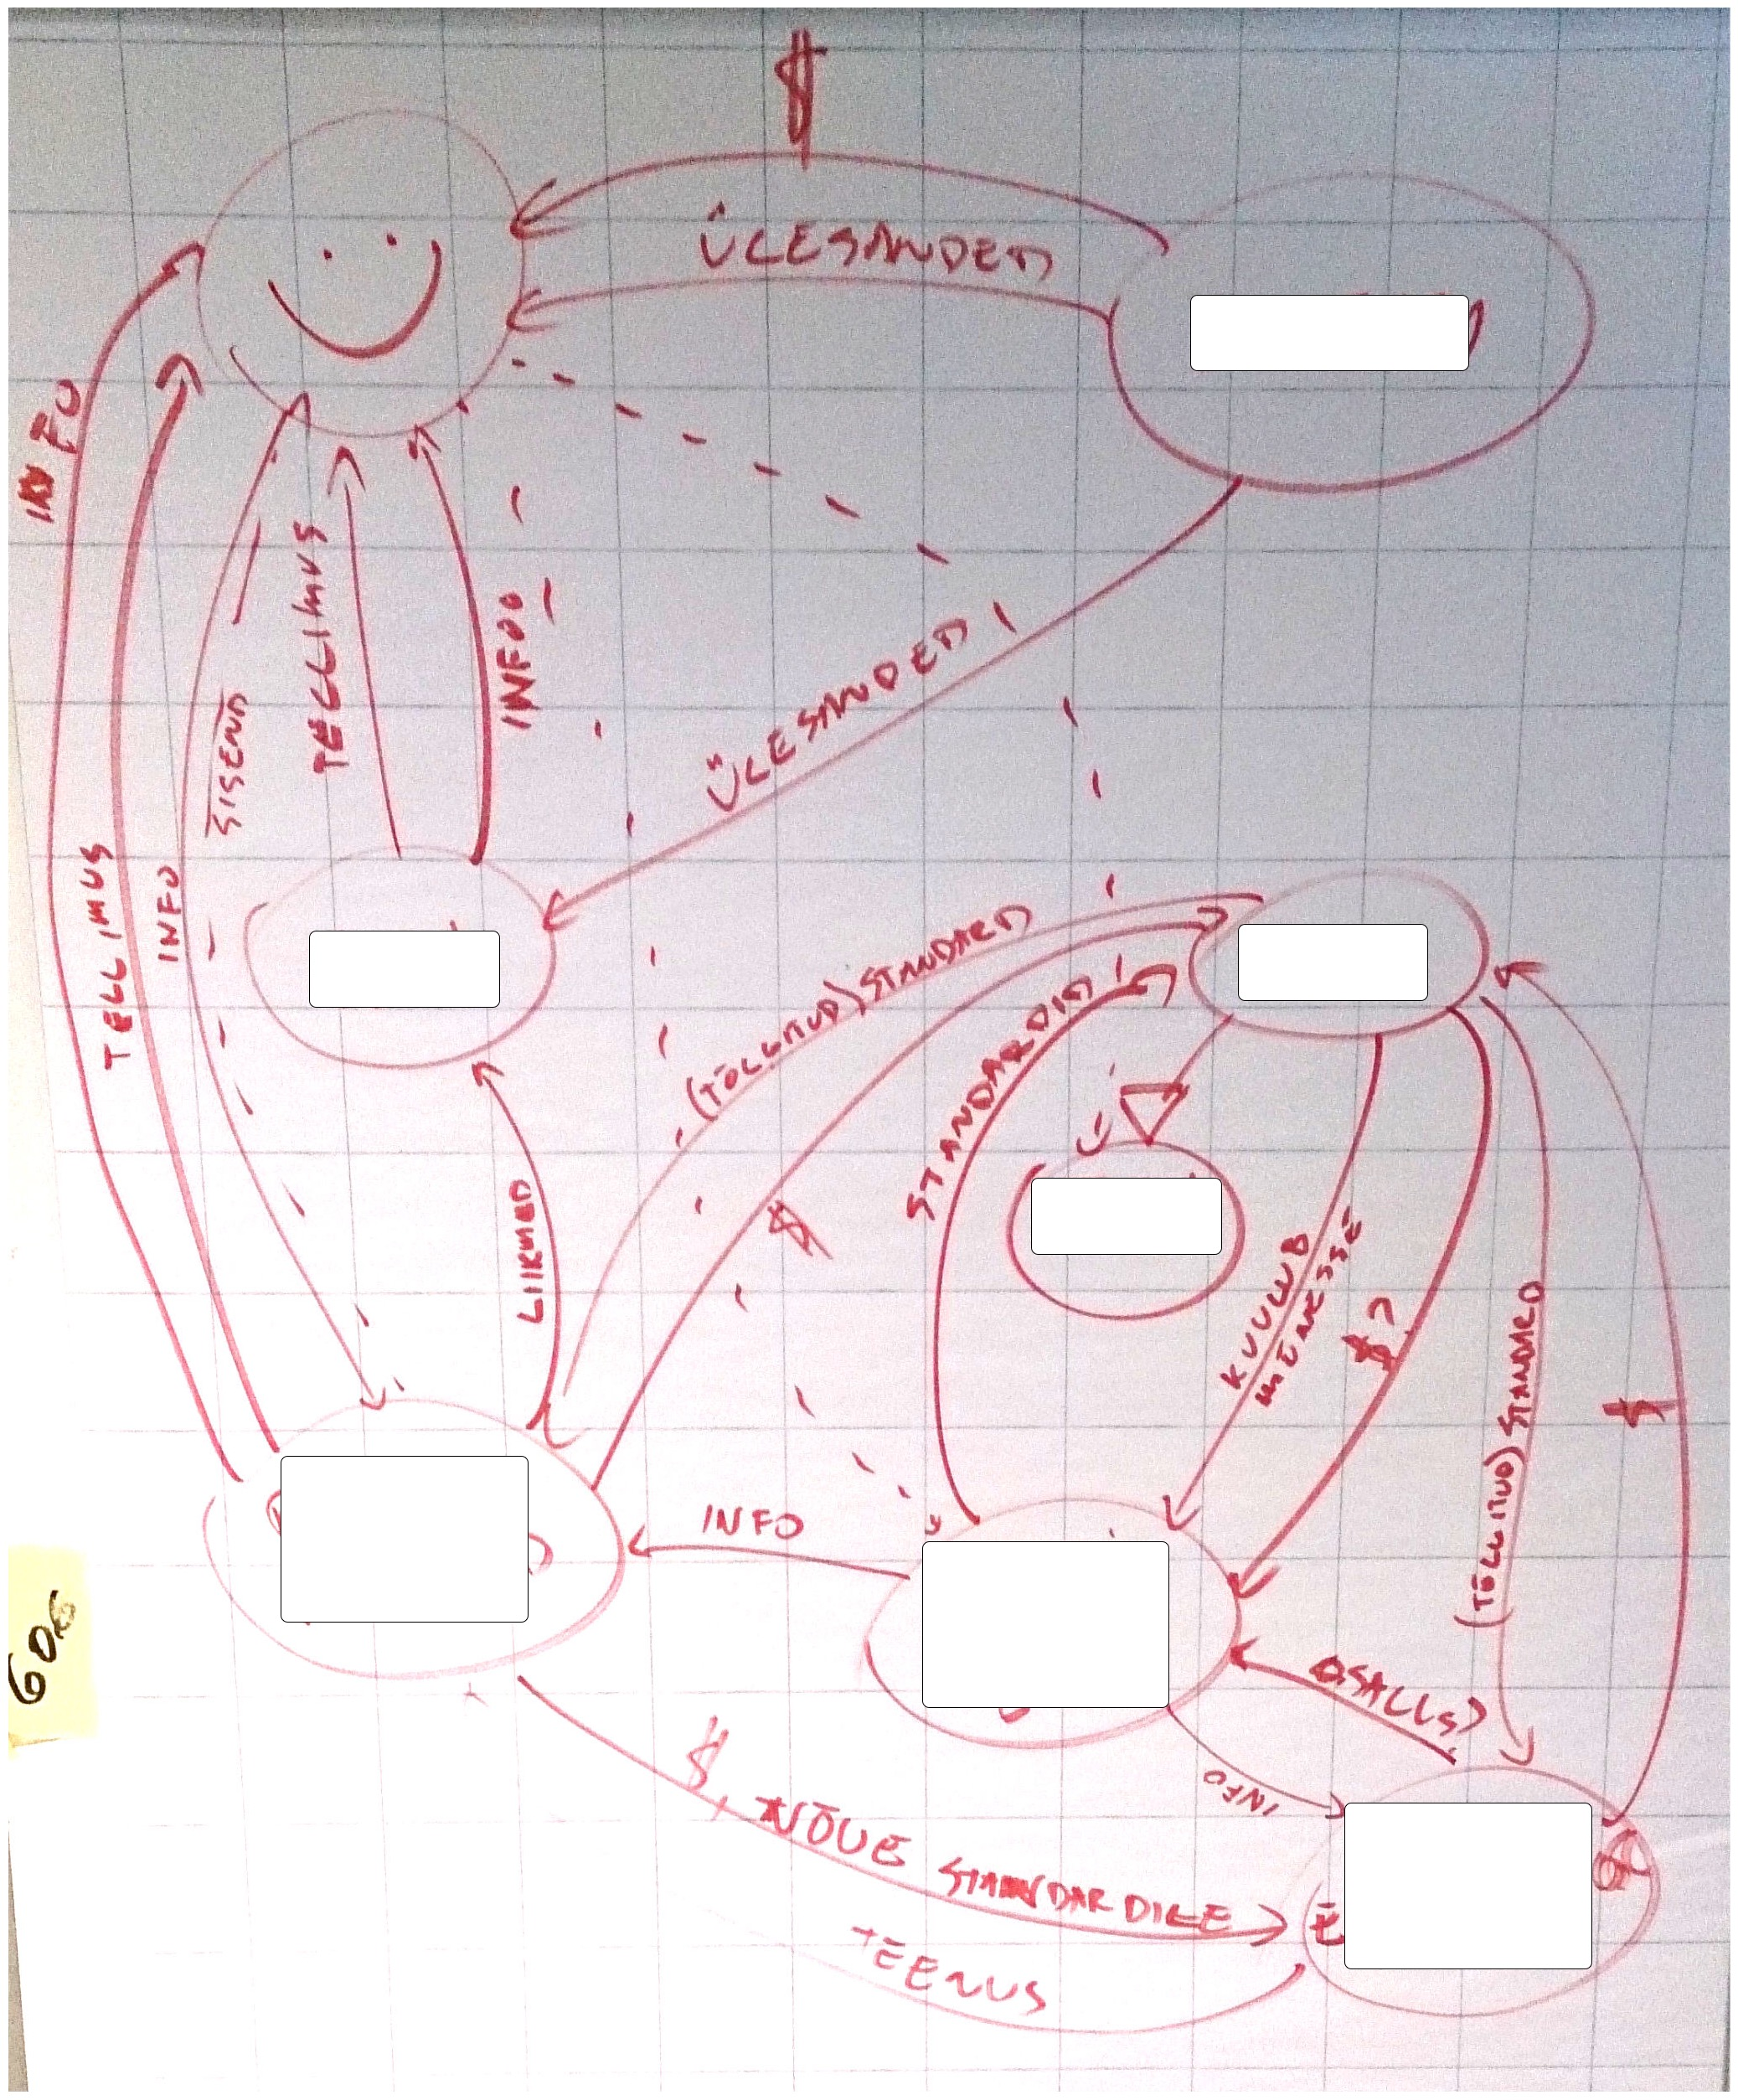
\includegraphics[width=.6\textwidth]{seosed.jpg}
		\caption{Näide seoste diagrammist}
		\label{fig:seosed}
	\end{center}
\end{figure}




\section{Piiridest ja nende ületamisest}
Eelmise sajandi seitsmekümnendatel töötas Jay Forrester Rooma Klubi tellimusel välja mudeli maailma rahvastiku kasvu uurimiseks. Forresteri õpilased on mudelit hiljem täiendanud, hetkel on ehk parim lugemismaterial \cite{meadows1992beyond}. Ennustused ei ole roosilised, pigem vastupidi. Ühe tõenäolise võimalusena nähakse ette, et rahavastik ületab suurelt piirid, mida tehnoloogia võimaldab planeedil Maa ära toita ning mahutada ja et järgneb mõõdukas kollaps. Rahvastik kahaneb kiiresti ning palju ning toimub tugev konkurents ressursside pärast (sest kõigile lihtsalt ei jätku). 

\section{Trammifaktor}
\index{Truck number}
Jätkusuutlikkust võib ka vaadata riskijuhtimise nurga alt. Sel viisil mõeldes on jätkusuutmatu olukord, kus organisatsiooni jaoks kriitiline risk on maandamata. Riskide ignoreerimine võib hästi lõppeda vaid piiratud aja jooksul.

Üheks tüüpiliseks IT-organisatsioonide riskiks on inimrisk. Ikka ja jälle leiame end olukorrast, kus kogu teadmine mingi valdkonna või süsteemi kohta on koondunud ühe inimese pähe\sidenote{Tüüpiliselt on tegemist tagasisidega: Kuna inimene teab süsteemist kõige rohkem, pöördutakse murega tema juurde. Mure lahenemise läbi suureneb tema teadmine süsteemist ja seega ka suhteline kompetents võrreldes teistega. Ja suureneb ka tõenäosus, et ka järgmine kord minnakse probleemiga tema juurde. Ta teab süsteemist seda rohkem, mida rohkem ta süsteemist teab.}. Tegu on niivõrd tüüpilise riskiga, et agiilses arenduses on olemas spetsiaalne termin - \emph{truck number}\cite{coplien2004organizational}. Eesti keelde võiks selle ehk tõlkida kui \enquote{trammifaktori}. Trammifaktor on maksimaalne tiimi liikmete arv, kelle trammi alla jäämine mõjutaks meeskonna jõudlust lineaarselt. Kui trammifaktor on üks, siis mõjutab õnnetus võtmeisiku oluliselt rohkem, kui lihtsalt tema panuse puudumine. Ideaalis on N-liikmelise meeskonna trammifaktor N-1, kuid praktikas nii hästi juhitud meeskondi tihti ei kohta. 

\section{Küsimused aruteluks}
\subsection{Miks on kõrge PUE oluline?}
PUE\sidenote{PUE - \emph{Power usage effectiveness} näitab, milline osa kogu kulutatavast energiast kulutatakse arvutustehnika käitamisele}\index{PUE} on küllalt populaarne viis andmekeskuste efektiivsuse hindamiseks. Kõige ilmselgemalt on tema maksimeerimine kasulik majanduslikult: kui PUE on üks, kulub kogu elektriarve arvutamiseks ja seega väärtuse loomiseks. Samas on PUE kasvatamine ka selgesti kahaneva piirkasulikkusega protsess\sidenote{Iga järgmine ühik PUEd tuleb kallimalt kui eelmine. Tegemist on dünaamiliste süsteemide puhul tavapärase asümptootilise lähenemisega sihile. Ehk, PUE küll saab ideaalile, ühikule, läheneda kuid ei saa ealeski kohale jõuda}. Järelikult nõuab PUE kasvatamine investeeringut. Loogiliselt võttes ei ole mõistlik investeerida rohkem, kui läbi energiasäästu tagasi tuleb\sidenote{Formaalselt tuleb lahendada võrrand $I_0=\sum_{t} \frac{C_t(I_0)}{(1+r)^t}$ $I_0$ jaoks. Ehk, igakuine sääst elektriarvelt peab meid huvitava perioodi jooksul intressimäära r juures võrduma algse investeeringuga. Paraku, nagu öeldud, on $C_t$ mittelineaarne funktsioon ja seega eeldab tasakaalupunkti leidmine tavaliselt suhteliselt keerukat stsenaariumide läbi arvutamist.}. Igasugune nüüdisväärtuse arvutus sõltub olemuslikult ka ajaperioodist ning seega oleme saanud seose ettevõtte toimetamise ajalise perspektiivi ning jätkusuutlikkuse vahel. 

Teine PUE kasvatamise põhjus võib olla keskkonnast tulenev. Kui kogu energia kulutatakse arvutamisele, peaks see ju vähendama organisatsiooni ökoloogilist jalajälge, vähendama koormust keskkonnale? Kindlasti on tegemist olulise põhjusega kuid tuleb teha vahet keskkonnasõbraliku maine ja reaalse keskkonnasõbralikkuse vahel. Nimelt mõõdab PUE energiaefektiivsust vaid andmekeskuse sees. Tuletades meelde diskussiooni süsteemi piiridest\index{Süsteem!Piirid} on lihtne näha probleemi. Nimelt võib küll andmekeskus toimida äärmiselt efektiivselt juhtides arvutamise käigus tekkivad jääksoojust keskkonda, kuid ta ei ütle midagi keskkonnas toimuva kohta. On suhteliselt lihtne disainida soojusvahetusele tuginev süsteem, mis talvel eraldab väga efektiivselt keskkonnas ruumide kütmiseks piisavalt soojust ning suvel viib liigsoojuse sinnasamma tagasi. Kuid kuna arvuti on ikkagi kütteallikas, võib maasse pumbatav energiahulk oluliselt ületada sealt võetava. Põhimõtteliselt köetakse serveriruumi ümbritsevat pinnast ning see ei pruugi ökosüsteemi vaatepunktist kasulik olla. 

Kui nüüd regulaator otsustab näiteks seada PUEle teatud sihtväärtused kuid ei rakenda piiranguid keskkonna mõjutamisele, saame täiesti ebasoovitava tulemuse. Energiatõhususe läbi keskkonnasäästu soovides tekitame keskkonnale koormuse, mille suhe saavutatud kokkuhoidu ei ole sugugi ilmne. Ettevõtte kuvand käitub sarnaselt regulaatoriga. Ka avalikkusel on teatav ootus ettevõtte teatud käitumise suhtes ning oodatud käitumise ning tegeliku kekskonnamõju vahel ei pruugi olla üksühest seost.

Juba suhteliselt lihtsa arutluse käigus ühest serveriruumi efektiivsusnäitaja üle tõusid esile keeruline mittelineaarne optimiseerimisülesanne, dünaamiline keerukus, küsimus ajahorisonidst ja avalikkussuhted. Küsimus terve ettevõtte jätkusuutlikkusest on veelgi keerulisem. 


\subsection{Kuidas tuvastada jätkusuutmatust?}
Lähtudes jätkusuutlikkuse definitsioonist \enquote{jätkusuutlik on tegevus, mida võib mingites ajaraamides sarnaste tulemustega jätkata} on jätkusuutmatuse täielik tuvastamine keeruline. Selleks on definitsioon liiga üldine. Küll aga võib suhteliselt kergesti tuvastada konkreetseid käitumisi, mille jätkusuutmatus tuleneb nende olemusest. Eksponentsiaalne kasv, näiteks, ei saa lõputult jätkuda, varem või hiljem saavad mingid ressursid otsa. Ülesande teeb lihtsamaks asjaolu, et süsteemide probleemid on reeglina endogeensed, seega võime välised tegurid rahulikult kõrvale jätta.

Millised siis on käitumised, mis ei ole olemuslikult jätkusuutlikud? Toetudes Senge\cite{senge19905th} süsteemiarhetüüpidele võib välja joonistada järgmised peamised jätkusuutmatud mustrid
\begin{description}
	\item[Piiratud kasv] Protsess toidab iseennast viies kiireneva kasvu või ekspansioonini. Ühel hetkel hakkab kasv aeglustuma kuni peatub või (ülereageerimise korral) muutub kiirenevaks kahanemiseks. Põhjuseks on üks või mitu välist tasakaalustavat mehhanismi. Näitena võib tuua MySpace'i\sidenote{Asutati 2003. aastal, oli 2005-2008 suurim sotsiaalvõrk maailmas} sotsiaalvõrgustiku. Mida rohkem seal inimesi käis, seda kasulikum oli kontot omada ja seda rohkem inimesi keskkonda ka külastas. Võrgustiku populaarsus aga tekitas järjest kasvava innovatsioonihuvi konkurentide poolt. Kuni ühel hetkel kerkis esile Facebook ning algne kasv pöördus. Mida vähem inimesi MySpace kasutajaks jäi, seda vähem oli seal põhjust käia.
	\item[Eskalatsioon] Kaks osapoolt näevad oma edu suhtelise ülekaaluna teisest. Mida paremaid tulemusi üks osapool saavutab, seda rohkem teine pingutab tõstes oma tulemust mis viib omakorda suurema pingutuseni esimeselt osapoolelt. On selge, et ühel hetkel sekkub piiratud kasvu stsenaarium ning olukord ei ole jätkusuutlik. Siiski on tavaliselt enne lõppu kulutatud palju rohkem ressursse, kui mõistlik oleks. Heaks näiteks eskalatsioonist on külma sõja aegne tuuma-arsenali kuhjamine. Hetkeks, kui Nõukogude süsteemi piirid kätte jõudsid, oli valmis ehitatud oluliselt rohkem relvastust, kui võiks eales sisulist väärtust omada.
	\item[Jagatud ressursi tragöödia] Osapooled kasutavad ühist kuid piiratud ressurssi. Seejuures on ressursikasutus end taastootev. Mida vähemaks jääb ressurssi, seda rohkem pingutatakse selle kasutamiseks ning seda intensiivsemaks ressursikasutus kõigi osapoolte poolt muutub. Lõpuks saab ühine ressurss otsa. Näitena võib tuua IT arenduse. Tavaliselt on tegemist eri osakondade jaoks jagatud ressursiga. Mida rohkem mõni osakond arendust vajab, seda edukam ta on ja seda suurem huvi on majasisese konkurentsi tingimustes ka teistel oma süsteeme arendada. Tulemuseks on IT-arenduse \enquote{pikali jooksmine} ning kõigi osapoolte võimekus midagi tehtud saada.
	
\end{description}

Kindlasti on erisuguseid jätkusuutmatuse näiteid veel, kuid kirjeldatud kolm katavad ära peamised süsteemide tüübid, mis oma käitumist lõputult jätkata ei saa.


\chapter{Muutused äris}

\section{Struktuursed ja mittestruktuursed muutused}
Analüüsides ärimuutust on oluline mõista, millistes organisatsiooni kihtides (Vt. joonis \ref{fig:stack} leheküljel \pageref{fig:stack}) on tegemist struktuurse ja millistes mittestruktuurse muutusega. Struktuurne on muutus, mis muudab kihi arhitektuuri samas kui mittestruktuurne jätab selle muutmata. Küsimus on oluline, sest arhitektuuri muutmine on, vastupidiselt olemasoleva arhitektuuri raames toimetamisega, reeglina kallis.

Võtkem näiteks ettevõtte, kes müüb oma teenuseid e-poe kaudu. Tehakse otsus, et veebilehele tuleb lisada võimalus klienditoega sõnumivahetusse asuda. Sellist funktsionaalsust pakkuvaid tarkvarapakette on palju ning nende integreerimine olemasolevasse tehnilisse lahendusse reeglina ei ole probleem. Tegu ei ole struktuurse muutusega, olemasolev arhitektuur jääb paika. Samas on organisatsioonis 24/7 toimiva klienditoe funktsiooni arendamine äriprotsesside ja organisatsiooni struktuuri mõttes üsna keeruline ettevõtmine. Tuleb palgata ööpäevaringse valve mehitamiseks piisav hulk inimesi ning nende juht, organiseerida juurdepääs kontoripinnale, tõeäoliselt tegeleda tööseadusandlusest tulenevate piirangutega jne. jne. Selgesti on tegemist arhitektuurse muutusega. 

Tüüpilisemad on vastupidised näited kus organisatsiooni vaatest triviaalne muutus võib osutuda tehnilises mõttes uut arhitektuuri nõudvaks. Otsused tulevad just organisatsiooni vaadet omavatelt inimestelt kes lihtsa muutuse palju suurema tõenäosusega ette võtavad kui keerulise. 

Et arhitektuuri mõiste ei ole hästi defineeritud ei ole ka struktuurne ja mittestruktuurne muutus selgepiirilised mõisted. Selge on siiski, et erinevad muudatused vajavad erineva hulga olemasoleva välja vahetamist ning just see on küsimuse iva.

\section{Keerukus ja keerulisus}
\TODO Kirjuta slaidide alusel lahti. Keerulisuse juures võimude pilt

\section{Kuidas mõõta infosüsteemi keerukust?}
\label{sec:complexity}
\cite{mitchell2009complexity} toob välja rea keerukuse mõõtmise viise. \citeauthor{crawley2015systems}\cite{crawley2015systems} toob välja mitmeid konkreetseid valemeid keerukuse arvutamiseks. Kuna variatsioone teema ümber on arvukalt ning nende erivused ei ole siinkohal määrava tähtsusega, kasutame keerukuse hindamisel järgmist valemit. 

\begin{equation}
	C = \sqrt[3]{N_e + N_et + N_s + N_st}
	\label{eq:complexity}
\end{equation}

\begin{itemize}
	\item $N_e$ on elementide hulk süsteemis
	\item $N_{et}$ on elementide tüüpide hulk süsteemis
	\item $N_s$ on elementidevaheliste seoste hulk süsteemis
	\item $N_{st}$ on elementidevaheliste seoste hulk süsteemis
\end{itemize}

Valemi sisu on lihtne: süsteemi keerukus määratletakse kui lineaarsest aeglasemalt kasvavat summat elementidest, seostest ja nende liikidest. 

Vaatleme selle valemi rakendamist lihta ülesande näitel. Olgu meil ülesanne liiklust läbi kahest komponendi - turvaserverist ja infosüsteemist - koosnevas süsteemis. Turvaserver saab väliskeskkonnast päringu ja edastab selle infosüsteemile töötlemiseks. Süsteemi põhimõtteline paigaldusskeem on toodud jooonisel \ref{fig:complexity:pure}.

\begin{figure}[htp]
	\begin{center}
		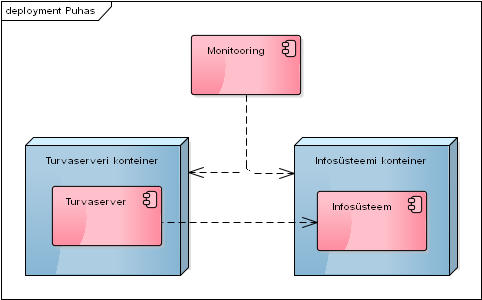
\includegraphics[width=.6\textwidth]{puhas.png}
		\caption{Jälgitava süsteemi põhimõtteline paigaldusskeem}
		\label{fig:complexity:pure}
	\end{center}
\end{figure}

Süvenemata realisatsiooni detailidesse võib öelda, et leidub kaks põhimõttelist viisi liikluse jälgimiseks. Esimene koosneb eraldi paigaldatavast vahendajast turvaserveri ja infosüsteemi vahel. Vahendaja pakub sama liidest, mis infosüsteem ja edastab ühele poole päringuid ja teisele vastuseid. Teine koosneb turvaserveri ümber mässitavast lahendusest, mis jälgib turvaserverisse sisenevat liiklust ning edastab selle turvaserverile. Peamine vahe alternatiivide vahel on eraldi (virtuaal)serveri vajadus esimesel juhul. Alternatiivid on toodud joonisel \ref{fig:complexity:added}.


\begin{figure}[ht]
		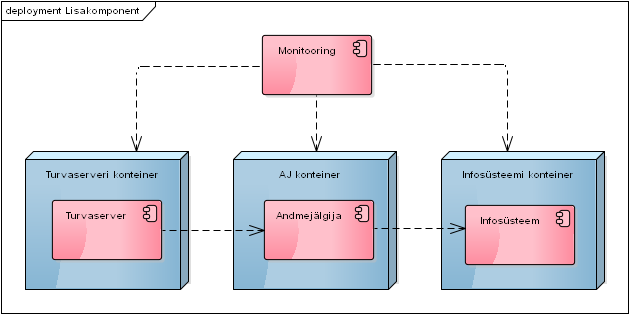
\includegraphics[width=8cm]{lisakomponent.png}
		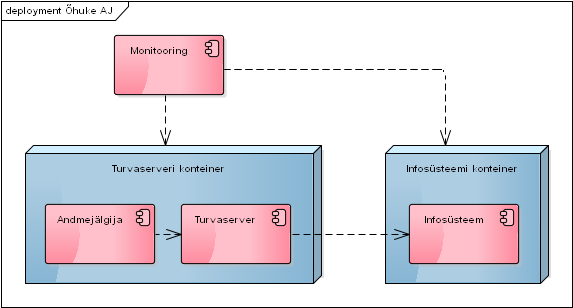
\includegraphics[width=8cm]{ohuke.png}
		\caption{Kaks alternatiivi andmete jälgimiseks}
		\label{fig:complexity:added}
\end{figure}

Esmapilgul ei ole alternativiide erinevus keerukuse mõttes ilmselged. Loendades valemi \ref{eq:complexity} muutujate väärutsi ilma andmejälgijata leiame, et süsteemis on viis elementi (kaks konteinerit ja kolm tarkvarakomponenti), neli liidest (turvaserveri sisenev, infosüsteemi sisenev ning monitooringuliidesed) ning et nii elemente kui liideseid on kahte tüüpi. Eraldi paigaldatava andmejälgija puhul saame vastavalt väärtused 7, 7, 2 ja 2. Õhukese lahenduse puhul väheneb küll elementide arv kuid lisandub uus liidese tüüp protsesside vaheliseks suhtluseks konteineri sees. Tulemused võtab kokku tabel \ref{tab:complexity}. 

Näeme, et andmejälgija iseenesest lisab süsteemi oluliselt keerukust. Samas on alternatiivne, turvaserveriga kokku paigaldatav, lahendus õige pisut väiksema keerukusega. Loomulikult on tegu lihtsustatud näitega kuid tegu on reaalse viisiga kvantifitseerida arhitektuursete lahenduste erinevusi. Tasub ka tähele panna, et süsteemi piiride määratlemisel on oluline mõju: kui lugeda süsteemi keerukuse hulka ka turvaserverisse sisenev liides, suureneb alternatiivide poolt jagatud liideste hulk ning seega väheneb suhteline erinevus. 

\begin{table}
	\begin{center}
		\begin{tabular}{p{3.6 cm}rrr}
		\toprule
& Puhas & Eraldi AJ & Õhuke AJ \\
		\midrule
Elemente ($N_e$) &	5 &	7 &	6\\
Liideseid  ($N_s$)	& 4 &	7 &	6\\
Elementide liike  ($N_{et}$)&	2	&2	&2\\
Liideste liike  ($N_{st}$)&	2 &	2 &	3\\
		\midrule
Keerukus &	2.35 &	2.62	 &2.57\\
		\bottomrule
		\end{tabular}
		\caption{Kokkuvõte alternatiivide keerukusest}
		\label{tab:complexity}

	\end{center}
\end{table}


\section{Küsimused aruteluks}
\subsection{Kas IT saab algatada organisatsiooni äri muutuse? Kui jah, siis kuidas?}
Üheks viisiks küsimuse üle arutleda on tagasipöördumine süsteemi kolme aspekti - vormi, funktsiooni ja kontseptsiooni - juurde. Nagu räägitud, annab kontseptsioon aluse vajaliku funktsionaalsuse realiseerimiseks konkreetse vormi abil. Kuna sama funktsiooni võib täita mitu vormi ja vastupidi, vajame kontseptsiooni, mis kahe hulga vahele seose tekitaks. 

Siit järeldub, et ka konkreetset funktsiooni realiseeriv vorm võib täita erinevaid funktsioone. Nuga loodi algul ilmselt tööriistana kuid võeti kiiresti kasutusele relvana. Ja siit tulebki üks IT võimalustest äri muuta: kui olemasolev vorm suudaks lisaks planeeritule veel midagi, saaks tolle miski äriks keerata investeerimata sentigi vormi muutusse ning kohandades vaid kontseptsiooni. 

Heaks näiteks on e-residentsus\index{E-residentsus}. Kuna kogu ID-kaarti ja e-teenuseid toetav taristu on igal juhul olemas (ning koormuse mõttes väga kaugel skaleeruvusprobleemidest) ei nõua paljut nonde kaartide välja andmine kellele iganes. Muutes riigi kodaniku kontseptsiooni\index{Kontseptsioon}, saab sama vormi abil realiseerida oluliselt laiemat funktsiooni. 

Siit ei tulene, et kogu loodav vorm peaks olema nii laia kasutusvõimalusega, kui võimalik. Tihti nii mõeldakse ja tulemuseks on kasutud platvormid, üliabstraktsed \enquote{konfigureeritavad} süsteemid ja, laias plaanis, üleinvesteerimine ITsse. Vorm peab olema optimaalne olemasoleva kontseptsiooni piirides. Järelikult on IT ülesanne lisaks potentsiaalsete uute funktsioonide tuvastamisele ka sellise süstemi kontseptsiooni arendamine, mis viiks võimalikult \enquote{lahtiste} ja mitmekülgsete vormideni. Kuigi kontseptsioon tuleneb suurel määral organisatsiooni kultuurist, on teda konkreetsetel juhtudel siiski võimalik mõjutada peegeldades kliendile tagasi sisendist mõnevõrra üldisemaid kontseptsioone. 

Ka siin tuleb loomulikult silmas pidada arenduse-halduse-äri kolmikut ning anda endale aru, millal soov kontseptsiooni arendada on tegelikult maskeeritud soov endale monumenti ehitada.

\subsection{Mida teha, kui ees olev muutus viib organisatsiooni teisele poole oma võimete piiri?}
Keerukusel\index{Keerukus} on komme eksponentsiaalselt kasvada (vt. joonis \ref{fig:complexity:growth}) ja nii võib kergesti juhtuda, et seni edukalt astutud sammudest järgmine viib meid teisele poole meie võimete piiri. Tulemuseks on meie võimetus süsteemi (nii tehnilist kui organisatsioonilist) hoomata ning seega ka juhtida. 

\begin{marginfigure}
		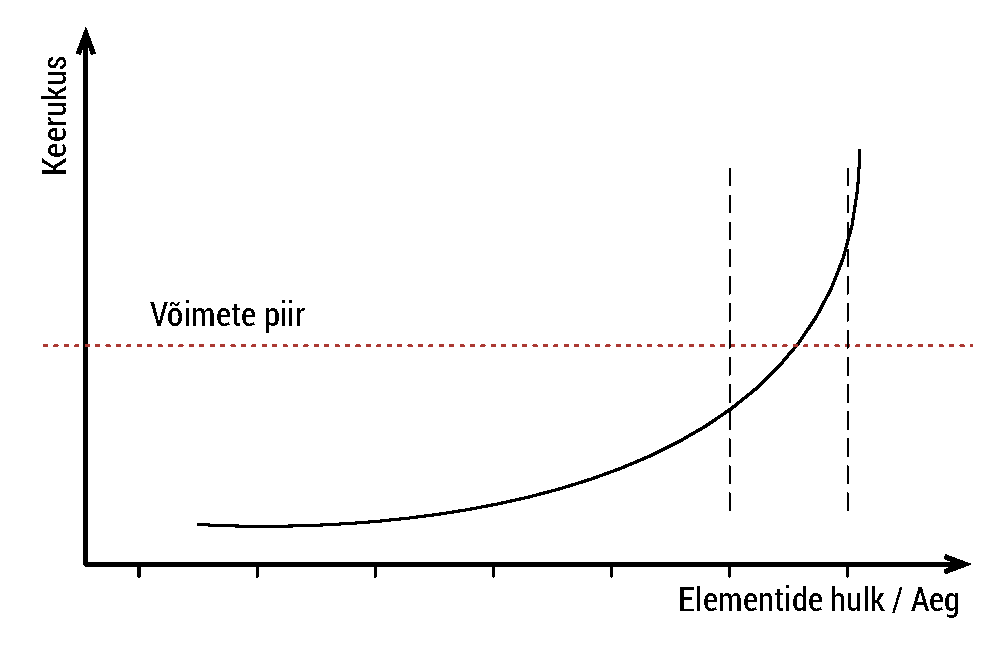
\includegraphics[width=\linewidth]{keerukus.pdf}
		\caption{Keerukuse eksponentsiaalne kasv teisele poole võimete piiri}
		\label{fig:complexity:growth}
\end{marginfigure}


Püstitatud küsimus on oluline, sest, eriti avalikus sektoris, ei ole muutus äris tihti ei välditav ega mõjutatav. Kui demokraatlik protsess on mingi tulemuse andnud, tuleb sellega leppida. Seda ka siis, kui organisatsioon seda välja ei kannata. Ideaalis muidugi võetakse organisatsiooni võimekust muudatust algatades arvesse kuid ei avalikus- ega erasektoris seda reeglina ei juhtu. Põhjuseks enamasti, et ei suudeta eristada objektiivset subjektiivsest. Ehk, kas läks vussi seepärast, et elluviijad osutusid saamatuks või seepärast, et ülesanne oligi antud kontekstis lahendamatu? Esimene variant on kindlasti käepärasem ning tavaliselt on otsustajate puhul mängus olulised positiivset mõtlemist soodustavad tegurid. 

Kuidas ka ei oleks, oleme me vastakuti muutusega, mis ei saa hästi lõppeda. Valgus tunneli lõpus on rong. Mida siis teha? 

Keerukuse juhtimiseks on meil juba mudelist tulenevalt kolm põhimõttelist strateegiat:
	\begin{description}
		\item[Google mudel:] \index{Google}Joone tõusu vähendamine. Me mõtleme välja, kuidas iga järgmine samm meie keerukust järjest vähem suurendaks. Kui google lisab oma farmi järgmise serveri, ei muuda see nende jaoks suurt midagi\sidenote{Google tarvitab oma serverite jaoks suurusjärgus 260 gigavatti võimsust (\url{https://www.technologyreview.com/s/425384/what-it-takes-to-power-google/}), ka massiivse gigavatise serveriruumi käivitamine ei muuda suurt midagi}. Ka järgmise teenuse või isegi äriliini käivitamine on tehtud suhteliselt lihtsaks. Google kogu äriedu tugineb nende võimel teha asju väga suurtes mastaapides, hoida oma keerukuskõver lamedana.
		\item[Morgani mudel:]\index{Morgan Motor Company} Peatumine horisontaalteljel. Briti autotootja Morgan on teinud põhimõttelise otsuse mitte areneda. Kasvu, keerukama tehnoloogia ja seega suurema tehnilise ja organisatsioonilise keerukuse asemel on jäädud piiratud mahtude ja käsitsi puust raamile loodavate autode juurde. Kindlasti on nii seatud piirid käibele (Morgan on perefirma ja seega täpseid arve saadaval ei ole) kuid kapitali tootluse mõttes ei pruugi tulemus olla sugugi halb
		\item[Skype mudel:]\index{Skype} Võimete piiri tõstmine. Nagu ka Google puhul, ei tähenda ka sadade miljonite uute klientide lisandumine Skype jaoks suurt midagi. Saavutatud on see aga teisiti. Skype on investeerinud äärmiselt keerulisse \emph{peer-to-peer} võrku\sidenote{Mille kohta on tänaseni vähe avalikult kättesaadavat pädevat informatsiooni. Lühidalt öeldes suudavad eri seadmetes käivitatud Skype kliendid omavahel suhelda ilma kekserveri vahenduseta. Kahe Skype kliendi vahel leitakse alati interneti mõttes lühim tee.}. Selle võrgu arendamiseks ja juhtimiseks piisab väga väikesest meeskonnast kuid kasutatav tehnoloogia on ülikeeruline ja seega on kõrged ka nõudmised kompetentsile.
	\end{description}

Kui muutus on juba meie poole teel, ei ole ükski neist paraku enam rakendatav. Skype ja Google mudelid eeldavad teadlikke arhitektuurseid otsuseid organisatsioonide varases arengufaasis ja Morgani mudel (sisuliselt vastuhakk muutusele) ei pruugi olla praktiline. \sidenote{Eestis on siiski vastav näide olemas. Eesti ühinemisel Euroopa Liiduga 2004. aastal kasvas maksu- ja tollivaldkondade infosüsteemide hulk kahelt neljateistkümnele. Kindlasti oleks tulemus olnud väljaspool kummagi ameti taluvuspiire. Seetõttu loodi uus organisatsioon, maksu- ja tolliameti ühine IT osakond, mis uued süsteemid ehitama ning omavahel siduma pidi. Ehk, tekkis võimalus disainida uus, juba suurema keerukuse taluvuse võimega, organisatsioon.}

Järelikult tuleb valmistuda tegelema meie võimeid ületava keerukusega. Definitsiooni järgi ei saa meie tegevus olla lõpuni edukas, kuid \enquote{küüsi maasse lüüa} õnnestub kindlasti. Mida siis saab teha 
\begin{description}
	\item[Dokumenteeri] Kuigi me ei pruugi olla võimelised süsteemi hoomata, võime vähemalt üles kirjutada, kuidas ta toimib. Kuigi tervikpilt on kadunud, on üksikute elementide toimimisest võimalik saada faktidele toetuv ülevaade. Seejuures tuleb vältida dokumentatsioon hoomamatuks ei kasvamist ning dokumenteerida ka mittetehnilisi süsteemi osi nagu äriprotsessid või suhtevõrgustikud
	\item[Lihtsusta] Süsteemi lihtsustamine (ehk, joone allapoole surumine) ei ole tavaliselt piisavalt kiiresti võimalik kuid kindlasti on võimalik oma keerukuse allikatele otsa vaadata ning mõnedega ka tegeleda. Näiteks võime teha otsuse loobuda majas arendatud rakendusest standardse lahenduse kasuks või asendada efektiivne kuid keeruline äriprotsess kuluka kuid suhteliselt lihtsa käsitööga
	\item[Planeeri] Muutus on võimalik kindlasti hoolikalt ette valmistada pöörates lahenduse disainil erilist tähelepanu lihtsusele. Samuti on võimalik muutust täide viiv projekt üles ehitada tavalisest konservatiivsemalt jagades tegevuse väikesteks etappideks, monitoorides riske ning jättes raha- ja ajalisi puhvreid. Oluline on siinkohal, et projekt kui selline ei pruugigi keskkonna keerukuskollapsit riskina tajuda: samalaadseid muutusi on ju varem probleemideta läbi viidud. 
	\item[Plaan B] Üheks liig keeruliste muutuste omaduseks on, et neid ei pruugi olla võimalik lõpuni läbi viia. Liigne keerukus võib edasise muutmise kas keeruliseks või hoopis võimatuks teha. Selleks puhuks on mõistlik omada alternatiivset plaani: mida me teeme, kui vältimatu ärilise muutuse tehniline realiseerimine (tähtaegselt) ei õnnestu?
\end{description}

\subsection{Kas strateegilised otsused peaksid olema ratsionaalsed?}
\TODO: täida sisuga
Ei, ei pea. Ja ka ei ole. Teatud piirini. Kui on paradigmamuutusega tegemist, siis ei saagi tihti ratsionaalne olla. Ja organisatsiooni kultuur ei pruugi ratsionaalseid otsuseid toetada. Ja meie võimekus ennustada ei pruugi olla suur ja järelikult me ei saa võtta vastu lõpuni ratsionaalseid otsuseid (tänane ratio ei pruugi homme seda enam olla). Mugavustsoon: kui olen miski asja juba ratsionaliseerinud, on tulemust hea kasutada. Kuigi tehtud eeldused enam ei kehti.

\chapter{Riskijuhtimine ja infoturve}
Järgnevas on olulisel määral toetutud Riigi Infosüsteemi Ameti spetsialistide sisendile, mille eest autor on põhjatult tänulik.

\section{Paradigmamuutus}
Riskijuhtimise paradigmamuutust tingivad järgmised trendid:
	\begin{itemize}
		\item BCP\footnote{\emph{Business Continuity Plan}} keerukus/hind kasvab eksponendina süsteemi keerukusest
			\begin{itemize}
		\item Facebookil ei ole kuskil teist andmekeskust igaks juhuks jõude seismas. See oleks liiga kallis
		\item Väliste partnerite puhul ei ole alati võimalik alternatiivi leida
		\item Äriprotsesside toimimisele ei ole vahel enam mitte-elektroonilist alternatiivi
	\end{itemize}

		\item BCP efektiivsus kahaneb eksponendina süsteemi keerukusest
			\begin{itemize}
		\item Kuidas taastub pilveteenusepakkuja täielikust andmekaost?
		\item Keerulist süsteemi ei pruugi õnnestuda ka mitte ajuti taastada, kui palju ka ei kulutaks. Kui Skype p2p võrk päriselt maha kukub, seda sisuliselt ei olnud võimalik taastada
		\item Äriplaanid, kliendiandmed, ideed, dokumentatsioon on üha enam immateriaalne ja seega kergesti teisaldatav
	\end{itemize}

		\item Üksikute riskisündmuste asemel peame rääkima pidevast, kasvavast ja kuju muutvast survest
			\begin{itemize}
		\item Ka kuritegevuses on edukas see, kes suudab oma ärimudeli võimalikult efektiivselt võimalikult suureks skaleerida
		\item Keerulises süsteemis on väga palju elemente ja nende interaktsioone, mõne katki mineku tõenäosus on suur
		\item Inimese kognitiivset võimet ületavate süsteemide puhul kasvab kiiresti operaatori vigade tõenäosus. Mistõttu ma olen suhteliselt ettevaatlik Eesti Vabariigi infosüsteemi torkimisega
	\end{itemize}

		\item Riskifaktoreid ei saa enam suruda aktsepteeritavale tasemele
			\begin{itemize}
		\item Riik suudab tagada, et tänaval ei jookse nagaaniga vehkiv jõuk, internetis ei ole see võimalik
		\item Süsteemi kõik elemendid ei ole kontrolli all. Vt. esimese kontakti slaidid Yosemite intsidendist
		\item Kuna info liigub, kerkib kiiresti esile uusi (Google: \emph{"ATM gas attacks"})
		\item Turvalist ega vigadeta tarkvara ei ole reaalne toota. Heartbleed istus aastaid laialt kasutatud open source tarkvarateegis kõigi silmade all
	\end{itemize}

\end{itemize}

\section{Süsteemiohutuse vaatenurk}
Eelnevalt loetletu kõrvale seab \cite{leveson2011engineering} oma nimekirja asjaoludest, mis sunnivad loobuma senistest süsteemide ohutust käsitlevatest mudelitest:
\begin{itemize}
	\item Kiire tehnoloogiline muutus
	\item Vähenev õppmisvõimekus, mida põhjustab järjest lühenev toote elutsükkel
	\item Õnnetuste iseloom on muutumas, eriti tänu tarkvara tihedasse integreerumisse igapäevaellu
	\item Uued ohtude tüübid. Nanotehnoloogia, keemia, antibiootikumid jne.
	\item Suurenev keerukus ja seotus
	\item Vähenev tolerants üksik-õnnetuste suhtes, mis tuleneb süsteemide suurusest ning meie suurenevast sõltuvusest tehnoloogiast
	\item Prioriteetide seadmise ja valikute tegemise keerukus
	\item Inimeste ja automaatide järjest keerulisemad suhted
	\item Muutuv regulatiivne ja avalikkuse vaade ohutusele. Üksikindiviid ei ole enam suuteline oma vahetu keskkonna ohutust kontrollima
\end{itemize}

Ta jõuab järeldusele, et süsteemi ohutus ja turvalisus on süsteemi emergentsed omadused. Seejuures tuleb süsteemi all mõista terviklikku sotsiotehnilist süsteemi\footnote{Süsteemi piiride kohta vt. \nameref{sec:boundary}}, mis sisaldab hulka omavahel suhestuvaid tehnilisi ja mittetehnilisi elemente. Sedalaadi mõtteviisi\footnote{Süsteemiohutuse kohta loe lähemalt kolmanda loengu slaididest} juured on sügaval ulatudes USA ICBM\footnote{Intercontinental Ballistic Missile - Mandritevaheline ballistiline rakett} programmi algusaegadesse. Tegu ei ole teoreetilise mõlgutusega, just tänu süsteemiohutusele on USA tuumalaevastikul seljataga 5400 reaktori-aastat intsidentideta tööd \cite{navy}. 

Süsteemiohutust rakendatakse edukalt ka küberturvalisuse valdkonnas. \citeauthor{hbrcyber} kirjeldavad just USA tuumalaevastiku kogemusele viidates, kuidas süsteemi turvalisus sõltub mitte ainult tehnilistest süsteemidest vaid ka inimeste koolitusest, neid sisaldavast organisatsioonistruktuurist, organisatsioonis toimivatest protsesidest jne. Ehk, tegeletakse süsteemi kui terviku turvalisusega.\cite{hbrcyber} 

Cook \citep{cook1998complex} võtab 18 punktis kokku keerulist süsteemide katki mineku olemuse. Eriti oluline on aru saada punktist 2: Rikke tõsised tagajärjed viivad selleni, et aja jooksul lisatakse järjest uusi kihte rikkekaitse mehhanisme. Tõepoolest: kuna ohutus on süsteemi emergentne omadus ei ole võimalik kõiki rikkeid ennustada ning kas rikked või rikkelähedased olukorrad viivad aja jooksul parema arusaamani võimalikest riketest. Siit tuleneb kaks olulist järeldust:
\begin{itemize}
	\item Kuna rikkekaitse mehhanismid on süsteemi osad, siis nende lisamisega süsteemi keerukus vältimatult kasvab (vt. ka peatükk \ref{sec:complexity}). Kuid süsteemi keerukus ja süsteemi ohutus on reeglina pöördvõrdelises seoses: keerukuse kasvades kasvab võimalike rikkestsenaariumide hulk. Ehk, kõikvõimalike kaitsemehhanismide lisamine suurendab süsteemi ohutust eksponenti mööda. Teatud piirist edasi ei suuda ka väga hästi konstrueeritud mehhanism süsteemi ohutust tõsta
	\item Eksisteerib konkreetne ja inimeste ohutusest tulenev surve süsteemi arendada lähtudes mitte selle algsest funktsioonist (ja seega ka arhitektuurist) vaid lähtudes ohutusest. Tegu on olulise ja juhtimist vajava survega süsteemi arhitektuuri terviklusele
\end{itemize} 

\section{Kaos ja ahvid}
Üks suurimaid probleeme slaididel ja loengus kirjeldatud paradigmamuutusega toime tulekul on inimeste hoiakud. Kui ühe serveri puhul võis loota, et see niipea katki ei lähe ja kui läheb, siis on teine varuks, siis 1000 serveri puhul läheb iga päev mõni katki. Sama lugu on küberrünnetega. Inimeste mõttemudel muutub aga aeglaselt. Probleemi on huvitavalt lahendanud Netflix \cite{monkey}. Nende vahend lihtsalt käib ja lülitab servereid välja, kõik teavad seda. Ehk, iga teenus peab olema suuteline sellist käitumist taluma. Sisuliselt on Netflix teadmata parameetritega rikete mürafooni asendanud palju tugevama kuid tuntud parameetritega signaaliga.   

\section{Küsimusi aruteluks}
\subsection{Milline on ohutu süsteem?}
\TODO: täida sisuga
Sellist asja ei ole olemas. 


\chapter{Infoturve}

\section{Korea isikukoodi näide}
2014. aastal tehti Lõuna-Koreas otsus vahetada välja isikukoodid\footnote{Lühike kokkuvõte ja edasisi viiteid saadaval siin \url{https://www.ria.ee/riigiarhitektuur/blog/2014/10/18/south-korea-about-to-overhaul-their-id-card/}}. Põhjuseks asjaolu, et sealne süstem oli üles ehitatud isikukoodi salajasusele. See viimane oli aga disainitud toetuma suhteliselt triviaalsetele turvameetmetele. Tulemuseks oli, et ühest küljest muutus isikukood ahvatlevaks ründeobjektiks ja teisalt olid rea intsidentide tulemusena kümne aasta jooksul sisuliselt kõigi kodanike isikukoodid lekkinud. Ja kuna identiteedivargus on üleüldine, tuleb isikukoodid välja vahetada.

\section{Infoturbe strateegiast}
Meid ümbritsevad infosüsteemid on muutunud ülimalt keeruliseks, organisatsioonid on erisugusest riist- ja tarkvarast põhjalikult läbi imbunud. Seetõttu on sisuliselt võimatuks muutunud täielik kontroll süsteemi üle. Heaks näiteks on väljakutsed BYOD\sidenote{\emph{Bring Your Own Device}, Too Oma Seade. Praktika, kus töötajad kasutavad töökeskkonnas isiklikke seadmeid. Tuntud ka kui \emph{Bring Your Own Disaster}, Too Oma Õnnetus} ümber ning sisuline võimekus tagada kogu organisatsioonis liikuva info varundamine. 

Samuti on tõsiasi, et kõigist paljudest komponentidest on mõni kogu aeg kas katki või siis ründele haavatav. Lahenduseks tundub olevat terviklik riskikäsitlus, sealhulgas süsteemi turvaliseks disainimine. Kuidas seda aga päriselt ilma kontolli omamata teostada? Head vastust anda ei ole, kui ehk võib abiks olla \citeauthor{leveson2011engineering}\cite{leveson2011engineering} ja tema mõtteviis ning arusaam, et keeruliste süsteemide puhul ei saa strateegiliselt eesmärgiks võtta totaalkaitset. Ehk, me ei ürita mitte kõiki süsteemi osa täielikult kontrollida ja kaitsta vaid maandame riskid \emph{piisavale} tasemele jättes teatud riskid teadlikult üles\sidenote{Avalikus sektoris on olukord teine. Seal ei saa asutus teadlikult aktsepteerida riski seadust rikkuda. Loomulikult jääb alati jääkrisk, millest me midagi ei tea, aga teadaolevat riski aktpseteerida ei saa. Kui me näiteks teame, et teatud krüptoalgoritm võib tulevikus murutud saada ja teame, et internetiliiklust salvestatakse, ei saa me näiteks rahvastikuregistrit selle algoritmi abil krüpteerituna internetti pidi edastada. Sest nii tehes võtame me riski avaldada isikuandmeid kolmandatele isikutele.}. 

Sedalaadi lähenemine eeldab aga ülevaadet süsteemi osadest, nende olulisusest süsteemi jaoks ning suhtelisest nõrkustest. Siit tuleneb aga jällegi küsimus süsteemi piiridest\index{Süsteem!Piirid}. Infoturbes lahendatakse probleem tüüpiliselt pragmaatiliselt: kui miski on oluliseks riski allikaks sellega ka tegeletakse.

Väga suurel määral sõltub infoturbega tegelemine infost (vt. ka \nameref{sec:valemid}). Järelikult on strateegiliselt oluline tegeleda riskide seirega. Ühest küljest tuleb jälgida oma süsteeme kuid vähemalt sama oluline on pidada silmas lähiümbruses (mis interneti mõistes ei tähenda loomulikult geograafilist lähedust) toimuvat. Siin on olulisel kohal mittetehniline seire: valdkonna kas avalikult või muul moel saada olev info tuleb pidevalt ohuhinnangute uuendamiseks ja prognooside tegemiseks läbi töötada. 

Eelnevat arvestades on selge, et infoturbe strateegia on tihedalt seotud paljude erinevate organisatsiooni toimimise aspektidega. OSA\sidenote{\emph{Open Security Architecture} on initsitatiiv, mis on eesmärgiks seadnud infoturbealase teadmuse avatud ja lihtsasti kasutatavateks mustriteks destilleerimise. Vt. \url{http://www.opensecurityarchitecture.org/cms/foundations/osa-taxonomy}} taksonoomia, kujutatud joonisel \ref{fig:osa} illustreerib seoseid ettevõtte strateegia, IT strateegia ja erinevate infoturbealaste tegevuste vahel. Tulemuseks on mõistete taksonoomia, mis võimaldab mõttestada infoturbe kohta organisatsioonilises kontekstis. Vaade on antud infosüsteemi vaatest, seega on näiteks kommunikatsioon pildilt puudu. 

\begin{figure}[h]
	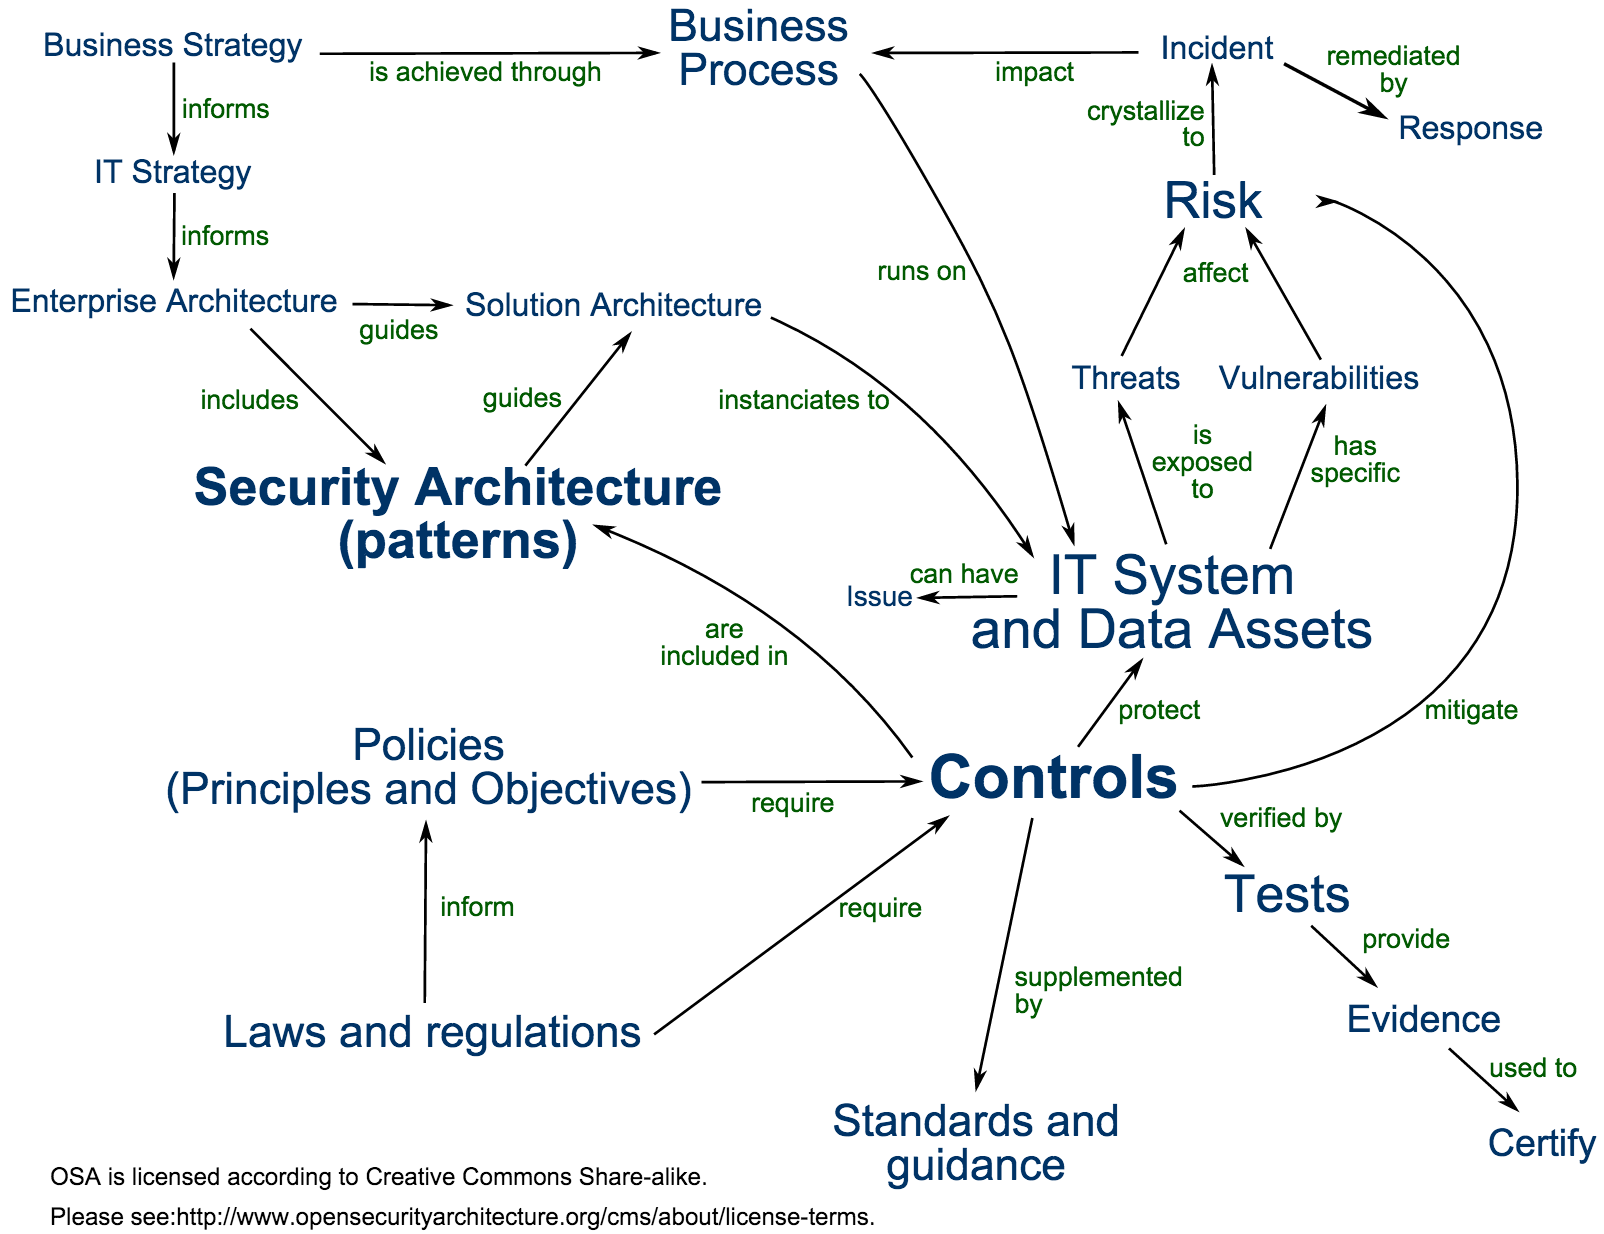
\includegraphics[width=\linewidth]{osa.png}%
	\caption{Seos äristrateegia ja infoturbe vahel OSA taksonoomia järgi} 
	\label{fig:osa}
\end{figure}

Sellel pildil on küll kesksel kohal infoturbe meetmed (\emph{Controls}), kuid sama olulised on erinevad infoturbe mustrid. Muster siinkohal on tavalisest üldisem mõiste tähendades suhteliselt üldist korratavat lahendust. Idee disainimustritest toodi esmakordselt välja füüsilise arhitektuuri valdkonnas\sidenote{\cite{alexander1977pattern} Paralleele infosüsteemide ja füüsilise ruumi planeerimise vahel on leitud ikka ja jälle. Mõnel juhul on nii üles ehitatud terveid metoodikaid:\cite{longepe2003enterprise}} ning OSA lähenemises on kesksel kohal infoturbe mustrite kataloog. Teine oluline tähelepanek on, et äristrateegiast tuleneb kaks olulist taksonoomia elementi: äriprotsessid, mida realiseerivad infosüsteemid ning EA\index{EA}, mis sisaldab infoturbe mustreid. Järelikult eeldab võimekus kaitsta infosüsteeme kooskõla äriprotsesside ja süsteemi arhitektuuri vahel. Mõistliku koostöö puudumine viib tõenäoliselt vastuolulini kus äriprotsess ei ole infoturbe mõistes kaitstav ärilises mõttes mõistliku määrani.

\section{Kuvandi olulisus infoturbes}
Nii valemi \ref{eq:tasuvus} (vt. lk \pageref{eq:tasuvus}) kui teiste riskimudelite puhul on olulisel kohal hinnangulisus. Ründajal on võimalik hinnata kohtuniku käitumist, õiguskaitse tõhusust ning kaitse taga asuva väärtust. Kuid tal ei ole võimalik neid teada. Järelikult on olulisel kohal infoturbes valemi parameetritest ebasoodsa mulje jätmine. Bütsantsi riik kasutas sama taktikat juba aastatuhandete eest, see toimib ka täna. Piltlikult öeldes võib seif olla valmistatud papist, kuid kuni kui kõik usuvad ta olevat läbimatust terasest, keegi talle kääridega ei lähene. Loomulikult on mulje ajutine ning raskesti juhitav ning seetõttu tuleb valmis olla selle purunemiseks. Kui levib info papist seifist, on maailmas kääre küllaga. Samuti ei ole ilmselt mõistlik tekitada kõrge väärtusega sihtmärgi kuvandit lisades ründest oodatavale kasule "feimi" komponendi. 

Jättes kõrvale pideva automatiseeritud ründevoo, võetakse järgmised sihtmärgid kõige tõenäolisemalt ette:
\begin{itemize}
	\item Ettevõtted, millede ründamine on moraalselt õigustatav, mis kuuluvad \emph{fair game} kategooriasse
	\item Ettevõtted, millede kohta on alust arvata, et küberrünne võib teha märkimisväärset kahju
	\item Ettevõtted, millede ründamisel võib olla laiemaid tagajärgi väljaspool sihtmärki
\end{itemize}

\section{Rünnete tõsidus}
Eri liiki ründed võib tõsiduse järgi jagada neljaks tasemeks, iga järgnev on eelmisest tõsisem

\begin{enumerate}
	\item Käitlustõrge (näiteks (D)DoS\footnote{\emph{(Distributed) Denial of Service} on rünne, mille käigus ülekoormatakse tahtlikult teenust pakkuv taristu kas ühesest või hajutatud allikast}. Samas on tegemist kõige kõrgema profiiliga ründega, sest paistab lihtsasti välja. Kui teenus puudub, on see kohe kõigile näha
	\item Teenuste ja äritegevuse toimimine mittesoovitud moel. Näiteks Stuxnet, mis ei seisanud rünnatavaid seadmeid, vaid muutis nende tööre\v{z}iimi ning kuvas juhtimismoodulile ebakorrektset infot. Samasse kategooriasse kuulub rünne haigla infosüsteemi vastu millega muudetakse haigete diagnoose, veregruppe jne. 
	\item Teenuse ja äritegevuse usaldusväärsuse langetamine. Kui teenuse usaldusväärsus langeb alla kriitilise piiri, teenust ei kasutata. Seejuures ei ole oluline, kas ja mil määral andmete terviklus või konfidentsiaalsus tegelikult ohus on. Eesti e-riik on selles osas suurepäraseks näiteks: meie riigi toimimine sõltub suurel määral usaldusest terve e-ökosüsteemi (riiklikud institutsioonid, pangad, id-kaart, tehnilised lahendused jne) vastu 
	\item Kontrolli kaotamine teenuse või äritegevuse üle. Sel puhul võetakse üle andmed, kaob kontroll äriprotsesside toimimise üle, teenuste käideldavus kõigub jne.
\end{enumerate}

Arusaam rünnete tõsidusastmest on oluline eriti tänases pidevate rünnete kontekstis. Kuna keegi kogu aeg ründab on oluline keskendada ressursid tegelemaks kõrgema taseme rünnetega. Madalama taseme ründeid võib kas lihtsalt ignoreerida (kui oluline ikkagi on asutuse veebilehe kadumine internetist?) või rahuldaval määral automatiseerimise abil kontrolli alla võttes näiteks paigutades niigi avaliku veebilehe mõne teenusepakkuja elastsesse pilve.

\section{Infoturbe valemid} 
\label{sec:valemid}
\subsection{Ründe tasuvus}
\begin{equation}
		S_p>P_f(S_a + P_c S_c)
		\label{eq:tasuvus}
\end{equation}

	\begin{description}
		\item[$S_p$] Ründest oodatav kasu
		\item[$P_f$] Ründe ebaõnnestumise tõenäosus
		\item[$S_a$] Ründe läbi viimise kulu
		\item[$P_c$] Vahele jäämise tõenäosus
		\item[$S_c$] Vahele jäämise kulu
	\end{description}

Toodud valemi puhul on oluline silmas pidada kahte asjaolu. 

Esiteks, et ründe ebaõnnestumise tõenäosus on reaalselt alati väiksem kui üks. Põhjuseks lihtsalt sotsiotehniliste süsteemide ülikeerukas olemus. Sihitud ja hoolikalt kavandatud ründe puhul ei ole küsimus selles, kas kaitsest suudetakse läbi murda. Küsimus on selleks kuluvas ajas ja ressursis ning läbimurde sügavuses. Silmas tuleb pidada ka ründevektori "ülevoolavust": alati valitakse ründeks kõige madalama kulu/tulu suhtega vektor. Süsteemide turvalisuse tõstmisega teatud piirist edasi suureneb lihtsalt sotsiaalrünnete surve ning süsteemi kui terviku turvalisus ei tõuse. 

Teiseks, muutujad on alati hinnangulised, neid ei ole ründajal võimalik otseselt mõõta. Siit tuleneb vajadus mõista ründajaid. Tegu on ju lõpuks nende poolt antud hinnangutega. Et eri osapoolte suhtelised võimekused ja huvid on erinevad, on erinevad ka nende hinnangud kulule ning ründest oodatavale kasule. On ju vahe, kas ründajaks on grupp internetiotsingut valdavaid teismelisi või mõne riigi APT\footnote{\emph{Advanced Persistent Threat} on varjatud ja pideva kübersurve oht, mis on suunatud konkreetse ospoole vastu} spetsialistid. 

Kuna evolutsioon dikteerib kõigi osapoolte huvi maksimeerida kasu minimeerides kahju võimaldab ründe tasuvuse analüüs hinnata kõige tõenäolisemaid sihtmärke ning seega planeerida kaitset: kuhu ja kui kõrged müürid ehitada. 

\subsection{Riski hinnang}

\begin{equation}
	RISK(Threat) = Threat \times Consequence \times Vulnerabilities
	\label{eq:risk}
\end{equation}

\begin{description}
	\item[RISK] hinnang riskile
	\item[Threat] hinnang ohule
	\item[Consequence] hinnang riski ohu realiseerumise tagajärgedele
	\item[Vulnerabilities] hinnang süsteemi haavatavusele
\end{description}

Valem \ref{eq:risk} ütleb, et risk on mittelineaarses sõltuvuses ohust, selle realiseerumise tõenäosusest ning süsteemi haavatavusest. Ehk, madala tõenäosuse kuid suure mõjuga oht, millele ollakse haavatavad on sama oluline kui kõrge tõenäosuse ja suure mõjuga oht, mille vastu ollakse hästi kaitstud. Samuti nähtub siit, et iga elemendi nulli viimine viib nulli ka riski. 

Nagu ka valemi \ref{eq:tasuvus} puhul, on siin tegu hinnangutega. Kuid erinevalt ründe tasuvusest on siin ebatäpne mulje pigem probleem, kui lahendus. Kui, eelnevalt kasutatud analoogiat jätkates, seif on papist, on seda kasulik teada ning mitte uskuda teda terasest olevat. Vastasel juhul on oht haavatavust alahinnata. Sama kehtib ka tagajärgede ja ohu kohta. Järelikult on täpne ning teadmistepõhine teadmine olukorrast adekvaatse riskijuhtimise puhul ülioluline.

Absoluutskaalade asemel võib valemi muutujate hindamisel kasutada suhtelisi. Näiteks võib toimida nii:

\begin{enumerate}
	\item Loetle ohud
	\item Anna igale ohule ohuhinnang skaalal 1-10
	\item Anna igale ohule sama skaalat kasutades tagajärje hinnang. Seejuures kata kinni ohuhinnang tagamaks muutujate sõltumatus
	\item Anna igale ohule haavatavushinnang kasutades jällegi sama skaalat ja kattes teised hinnangud kinni
\end{enumerate}

Nüüd oled igale ohule saanud suhtelise riskihinnangu, mis võimaldab neid sorteerida, valida maandamiseks jne.  

\subsection{Alternatiivide kaalumine}
\begin{equation}
	(B_1 - E_1) - (B_2 - E_2) > RISK(\varepsilon_1)-RISK(\varepsilon_2)
	\label{eq:alternative}
\end{equation}

\begin{description}
	\item[B] Kasu alternatiivi rakendamisest
	\item[E] Alternatiivi rakendamisega seotud kulud, sealhulgas riskide maandamiseks tehtavad kulud 
	\item[$\varepsilon$] Jääkoht, ehk ohud mis säilivad pärast kõigi meetmete rakendamist
\end{description}

Kuigi tavaliselt kasutatakse samalaadset valemit äriprojektide hindamisel (kasu peab üles kaaluma riskid) siis valemit \ref{eq:alternative} saab kasutada alternavtiivide hindamiseks. Siinjuures on oluline aru saada, et riski saab liigutada võrratuse paremalt poolelt vasakule ja vastupidi tehes või vähendades kulutusi jääkriski vähendamiseks või suurendamiseks. Teine kriitiline punkt siinkohal on ajaline mõõde: nii $B$, $E$ kui $RISK(\varepsilon)$ tuleb arvutada nüüdisväärtusena.

Olgu meil näiteks küsimus, kas võime oma andmeid hoida avaliku pilveteenuse pakkuja juures. Sel juhul 
\begin{itemize}
	\item $B_1-E_1$ on hinnang oma serverite pidamisest saadud kasule, millest on lahutatud serverite majutamise kulud (sealhulgas riskide maandamisele tehtavad kulutused). Kui oma serverite hoidmine iseensest tulu ei teeni, siis võib arvestada, et $B_1=0$. 
	\item $B_2-E_2$ on hinnang pilveteenusest saadavale kasule, millest on lahutatud tehtavad kulutused mis jällegi koosnevad nii riskide maandamiseks tehtavatest kuludest kui ka perioodilisest arvest. Jällegi, kui pilveteenus iseensest näiteks läbi parema käideldavuse kasu ei too, siis $B_2=0$
	\item $\varepsilon_1$ on jääkoht juhul, kui servereid majutatakse ise
	\item $\varepsilon_2$ on jääkoht pilveteenuse majutamise puhul
\end{itemize}

Pilve puhul me tõenäoliselt leiame, et riskid suurenevad, tekib teatav lisandväärtus ja kulud vähenevad. Küsimust pilve kasutamisest saab aga positiivselt otsustada vaid juhul, kui võrratus kehtib ning meie tegevuse tulud ületavad jätkuvalt riske.


\subsection{Oodatav kahju} 

	\begin{align}
		Annualised\ Expected\ Loss &= Frequency\ of\ a\ given\ attack\ type \label{eq:loss}\\
		&\times Potential\ Loss \nonumber \\
		&\times Extent\ to\ which\ the\ loss\ occurs \nonumber
	\end{align}


\begin{description}
	\item[Annualised Expected Loss] Oodatav aastane kahju
	\item[Frequency of a given attack type] Konkreetset liiki ründe esinemissagedus
	\item[Potential loss] Potentsiaalne kahju ründest
	\item[Extent to which the loss occurs] Potentsiaalne kahju keskmine realiseerumise määr
\end{description}

Valem \ref{eq:loss} võimaldab hinnata oodatavat kahju ründest. Teades, kui tihti ründed esinevad\footnote{Rünnete esinemise jaotus ning selle hindamine sisuliselt pidevate rünnete tingimustes on keeruline valdkond, millesse siinkohal liigne süveneda}, mis on neist tekkida võiv kahju ning mil määral kahju tavaliselt realiseerub, võib hinnata tekkivat kogukahju. Näiteks, kui meil on keskmiselt kaks tõsisemat teenustõrkerünnet aastas, mis kumbki võivad tekitada 10 000.- \euro kahju ning eelnev kogemus võimaldab hinnata, et kümmekond protsenti kahju õnnestub ära hoida on oodatav kahju $E(L)=2 \times 10000 \times .9 = 18 000$. 

Tegu ei ole infoturbespetsiifilise valemiga, täpselt samuti hinnatakse näiteks krediidiriske.



\section{Küsimusi aruteluks}
\subsection{Kuidas tellida turvalist tarkvara?}
\TODO: täida sisuga
Kui turvalisus ei ole süsteemi funktsioon vaid emergentne omadus, siis mida see tähendab tellimise jaoks? Emergents ei ole ju lõpuni ennustatav.


\chapter{Juhtimine}
\section{Partnerite juhtimine}
Enne, kui asuda end lahutamatult sisse söönud partnerist, "puugist", lahutama, on kasulik veidi mõelda. Asi võib olla selles, et koostöö võib parasiitluse asemel siiski sümbioosiks osutuda. 

On hea teha järgnevat:
\begin{itemize}
	\item Vii kas ise läbi või telli audit hindamaks süsteemi kvaliteeti ning strateegilist positsiooni. Hinnata tuleks nii koodi kui sellist, arhitektuurset lahendust kui ka süsteemi üldist avatust (dokumentatsiooni tase, APIde olemasolu jne.). Audit on kasulik ka sõltumatu argumendina põhjendamaks potentsiaalselt kõrgeid kulusid, mis süsteemide ümber kirjutamise või asendamisega paratamatult kaasnevad (vt. ka \ref{sec:rooste})
	\item Hinda alternatiive. ``Puugist`` lahti saamine ei ole väga mõistlik, kui järgmisel hankel jälle vaid seesama ettevõte tõsiseltvõetava pakkumise suudab esitada  
\end{itemize}

\section{Kvaliteedi juhtimine}
Kuna süsteemide puhul on reeglina tegemist sotsiotehniliste süsteemidega (st. süsteemi osaks loetakse ka lõppkasutaja) on oluliseks süsteemi kvaliteedi parameetriks nende kahe osise omavahaeline koostöö. Samuti väljendub süsteemi kasulikkus reeglina läbi lõppkasutaja. Järelikult on kasutajamugavus ja -kogemus kvaliteedijuhtimise olulised objektid. Reeglina toimub kasutajakogmuse disain süsteemi loomise algfaasis ning kvaliteedi tagamine selle lõpus, mistõttu kaks kompetentsi, paraku, reeglina kokku ei puutu.  

Tulemi kvaliteet sõltub olulisel määral kasutatavast protsessist, nii ka tarkvaras. Vt. \ref{humble}.

\section{Teenustaseme juhtimine}
Tavaliselt on organisatsioonides diskussiooni objektiks teenuse mõiste. Kuna kirjandusest samuti sobilikku määratlust võtta ei ole, siis võivad vaidlused osutuda pikkadeks ja viljatuteks. Seetõttu on oluline välja tuua teenuse definitsiooni kaks peamist struktuurset omadust lisaks slaididel kirjeldatud funktsionaalsetele omadustele:
\begin{itemize}
	\item Definitsioon peab suutma tõmmata selge, organisatsiooni ülevalt alla läbiva, piiri eri teenuste vahele
	\item Definitsioon peab olema vastuvõetav tervele organisatsioonile
\end{itemize}

samas:
\begin{itemize}
	\item Definitsioon ei pea olema täielik, määratletavad teenused ei pea katma kõiki organisatsiooni tegevusvaldkondi
	\item Definitsioon võib olla meelevaldne ("Teenuseks on rakendusse sisse logimine ja meie töötajate füüsiline kohalolu leti taga, miski muu teenus ei ole")
\end{itemize}

Kui esimesed kaks tingimust on täidetavad, võib vaidlused lõppenuks lugeda ning asuda teenustaset jutima.

\section{Projektijuhtimine}
Projektijuhtimine on väga keeruline teema ja sellest on kirjutatud palju. Siiski on mõned IT juhtimise vaatenurgast olulised asjad, millest on oluline aru saada. 

Võtkem näiteks projekti lõpptähtaja hindamise. Hindamine toimub tavaliselt nii, et projekt jagatakse sammudeks, iga sammu eest vastutaja annab oma hinnangu ja tulemus liidetakse kokku. Kõlab mõistlikult, eks? Kuid vaatame lähemalt. Iga vastutaja on tõenäoliselt kogenud inimene. Seega oskab ta anda hinnangu oma sammu mediaankestvust: kestvust, millest pooltel juhtudel õnnestub samm kiiremini läbida ja pooltel aeglasemalt. Eriti kogenud inimesed lisavad ka puhvri andes hinnangu, mis peab vett umbes neljal juhul viiest. Ühe sammu puhul on kõik hästi. Kuid kui samme on kaks? Et projekt ei hilineks, peaks oodatust kiiremini valmis saama \emph{mõlemad} sammud. Ehk, $P_{edu}=P(S_1\cap S_2)=P(S_1)P(S_2)=0.8\times0.8=0.64$. Üldisemalt, projekti hinnatust kiiremaks valmimiseks peab oodatust kiiremini valmima üks rohkem kui pooled sammud. Natuke arvutades saame, et viie sammu puhul on tõenäosus pisut üle poole ning kümne puhul juba veerandi ligi. Kokkuvõte on toodud tabelis \ref{tab:success}. Kuna vähegi keerukam it-projekt sisaldab sadu tegevusi\sidenote{Muidugi tuleb siin silmas pidada kriitilist ahelat, ehk ajaliselt pikimat üksteisest sõltuvate tegevuste jada projektis. Kuni muude tegevuste venimine uut kriitilist ahelat ei tekita, projekti lõpptähtaeg neist ei sõltu.} on üks olulisi projektide venimise põhjusi käes.

Juba paarikümne sammu puhul ütleb statistika, et projekti õigeaegselt või paremini lõppemise tõenäosus langeb kaheksa protsendi juurde. Ja seda eeldades, et sammude kestvuse jaotus on sümmeetriline. Mis aga kindlasti ei pea paika\footnote{\url{http://priceonomics.com/why-are-projects-always-behind-schedule/} toob ära jaotuse, mis põhineb 70 000 projektitundi sisaldava andmehulga analüüsil. Sealt on pärit ka toodud argumentatsiooni idee.}. 

Milles siis asi? Probleem on selles, et tõenäosuslikke muutujaid ei saa niisama lihtsasti liita. Tuleb aru saada, et hinnang projekti kestvusele on samuti tõenäosusjaotus nagu on seda ka üksikute sammude hinnangud. Kuna projekti tegevuste seosed on mittetriviaalsed, läheb jaotuste liitmine kiiresti liig keeruliseks. Agiilsed arendusmetoodikad keelduvadki tolle keerukusega tegelemast ja annavad lubadusi vaid lühikese ajaperioodi kohta. Siiski on ka mitte-agiilsete projektide puhul võimalik rääkida näiteks analüüsi, arenduse ja testimise sammudest millede jaotustega on võimalik tegeleda.  

Kindlasti aga tuleb vältida lihtsat hinnangute liitmist.

\begin{table}
	\begin{center}
\begin{tabular}{lll}

\toprule
Samme & Mediaan & 80\% hinnang \\
\midrule
1 & 0.5 & 0.8 \\
2 & 0.25 & 0.64 \\
3 & 0.25 & 0.64 \\
4 & 0.125 & 0.512 \\
5 & 0.125 & 0.512 \\
6 & 0.0625 & 0.4096 \\
7 & 0.0625 & 0.4096 \\
8 & 0.03125 & 0.32768 \\
9 & 0.03125 & 0.32768 \\
10 & 0.015625 & 0.262144 \\
11 & 0.015625 & 0.262144 \\
12 & 0.0078125 & 0.2097152 \\
13 & 0.0078125 & 0.2097152 \\
14 & 0.00390625 & 0.16777216 \\
15 & 0.00390625 & 0.16777216 \\
16 & 0.001953125 & 0.134217728 \\
17 & 0.001953125 & 0.134217728 \\
18 & 0.000976563 & 0.107374182 \\
19 & 0.000976563 & 0.107374182 \\
20 & 0.000488281 & 0.085899346 \\
21 & 0.000488281 & 0.085899346 \\
22 & 0.000244141 & 0.068719477 \\
23 & 0.000244141 & 0.068719477 \\
24 & 0.00012207 & 0.054975581 \\
25 & 0.00012207 & 0.054975581 \\

\bottomrule
\end{tabular}
		\caption{Projekti edukuse tõenäosus}
		\label{tab:success}

	\end{center}
\end{table}

\section{Reaalsusest, mudelitest ja juhtimisest}
Selleks, et midagi juhtida, peab meil olema mingit liiki mudel juhitavast objektist. Teeme ju eelduse, et muutes mõnda sisendit muutub väljund sobivas suunas. On oluline aru saada, et see mudel eksisteerib vaid meie peas ning on vaid reaalsuse lähendus. \citeauthor{box1976science} ütleb, et kõik mudelid on valed ja mõned mudelid on kasulikud\cite{box1976science}. Tema vana ütlemine on kahtlemata relevantne ka praegu ning artiklis toodud mudelid (kahtlemata valed kuid vahel osutunud kasulikuks) võimaldavad läheneda süstemaatiliselt objektide uurimisele. 

Lühidalt ütleb Box, et me kõigeapelt koostame teooria või mudeli reaalsuse kohta, siis disainime ja viime läbi eksperimendi mudeli valideerimiseks, saame uusi andmeid ning nende abil kohendame mudelit, millest tuleneb uue eksperimendi disain. Artiklis räägitakse küll teadlastest ja statistikutest kuid üldine lähenemine on  väga relevantne üldises keeruliste süsteemide juhtimise kontekstis: kirjeldatakse nii liigset teooriakesksust (vrdl. ``arhitektuursed astronaudid``) kui ka teooriapuudust ning rõhutatakse vajadust püsida kontaktis uuritava objektiga. Olulisimana jääb siiski kõlama vajadus eristada olemuslikult piiratud mudelit tema kirjeldatavast reaalsusest.  

\section{Küsimusi aruteluks}
\subsection{Kuidas vabaneda end sisse söönud ”puugist”?}
\TODO täida sisuga. Viide Aeda legacy tööle eespool. 

\begin{itemize}
	\item Kirjuta kogu asi korstnasse. See ei pruugi olla palju kallim (arvutused ja modelleerimine!)
	\item Osta ära
	\item Investeeri teadlikult muskli kasvatamisse ja arvesta kvaliteedi langusega
\end{itemize}

\subsection{Mida saab teha saamatu kliendiga?}
Eespool juba arutelu "kas saab ITd mõistlikult juhtida, kui klient ei ole mõistlikult juhitud?". Erista teadmiste/oskuste puudus võimete puudmisest (organisatsiooni, mitte isiku tasemel) Lolli tuleb kas kiita või temast lahti saada. Do not try to teach a pig to sing. It wastes your time and annoys the pig. 

\subsection{Millal on tarkvara valmis?}
Tarkvara on valmis siis, kui tehakse vastav otsus. Arendusprotsess vähegi mittetriviaalsel juhul ei koondu. Järelikult
\begin{itemize}
	\item Peab olema võimekus otsust teha
	\item Peab eksisteerima otsustusprotsess
	\item Peab otsustajatel olema mandaat ja pädevus otsustada. Seega peab otsustusprotsess kaasama kõiki osapooli (klient, opsid, ka arendaja) ja olema läbipaistev
\end{itemize}

\subsection{Milline tarkvara on kvaliteetne?}
\TODO täida sisuga

\subsection{Mis on teenus?}
ITIL\index{ITIL} defineerib teenuse mõiste omandi läbi: [teenus on] \enquote{väärtuse pakkumine klientidele võimaldades neil saavutada lõpptulemusi ilma kaasnevaid kulusid ja riske kandmata.}\cite{itil}. Ehk, teenust pakkudes võimaldadatakse kellelgi saada väärtust ilma, et ta peaks teatud kulusid ja riske ise kandma. Mõiste on olemuselt tautoloogiline sisaldades nii abstraktse kui kui konkreetse väärtuse pakkumist: teenuseid pakkudes pakutakse tegelikult kulude ja riskide kandmise teenust. Järelikult on teenuse pakkumise eelduseks võimekus mingil põhjusel pakkuda väiksemaid riske ja kulusid. Kuidas seda saavutatakse ning mis \enquote{teenus} tegelikult on, ei öelda. Siiski on definitsioonis olulisel kohal väärtuse ja seega ka kliendi mõiste, teenust ei saa osutada ilma kliendita.

ISO 20000\index{ISO 20000} on märksa ebamäärasem defineerides teenuse kui vahendid või meetodid, mida organisatsioonid kasutavad klientide poolt väärtustatud ja soovitud tulemuste saavutamiseks. \cite{iso20000}. Kuigi mängus on klient, ei ole enam tehtud eeldust, et klient teenuse tarbimise läbi rohkem väärtust saab kui tulemust ise tekitades. Oluline on ka tähele panna, et kui ITIL keskendub funktsioonile (\enquote{väärtuse pakkumine läbi...}) siis ISO vormile (\enquote{vahendid või meetodid}. 

Kindlasti on mitmesuguseid definitsioone veel, kuid ilmsesti on need kaks kõige levinumad ja osundavad kenasti levinud probleemile. Nimelt on tegemist juhtimise seisukohalt suhteliselt kasutute määratlustega. Neile on võimalik üles ehitada küll keerukas ja kõikehõlmav teoreetiline aparatuur kuid nad on praktiliseks kasutamiseks liiga hägusad. Kui teenus on \enquote{väärtuse pakkumine väärtuse pakkumiseks vajalike vahendite abil}, siis on see kahtlemata õige aga kuidas ja mis otsuseid me selle määratluse abil tegema peaksime? Kogu IT pakutav on vaadeldav kui üks teenus ja kindlasti on ka kuskil serveris käiv \texttt{cron} \enquote{vahend väärtuse pakkumiseks}. 

Mida siis teha? IT juht tegeleb reeglina mitte üksikute teenuste vaid teenuste portfelliga. Portfelli kui terviku ja selle üksikute elementide jõudlust peaks olema võimalik hinnata ning teha otsuseid. On selge, et ühest elemendist koosnev teenusteportfell lükkab teenustega tegelemise lihtsalt kellegi teise õlule. Samuti on ilmselt igal inimesel ja organisatsioonil konkreetses tehnoloogilises kontekstis võimalik hoomata piiratud hulka teenuseid. Rohkemaid teenuseid küll võib defineerida aga sellest ei saa palju kasu olla: juhtimislikke otsuseid on võimalik teha ainult hoomatavuse piires. 

Seega jõuame veidi praktilisema teenuse definitsioonini: \enquote{Teenus on miski, millest ja millesarnastest on võimalik koostada praktiliselt kasulik teenuste portfell}. Seejuures on täitsa ükskõik, kas lähtutakse ITILi, ISO või mõnest kolmandast teenuse definitsioonist. Samuti on oluline mõista, et eri organisatsioonide portfellijuhtimise võimekus on erinev. Hästiarenenud EA\index{Enterprise Architecture} taristu abil on võimalik tegeleda tuhandete teenustega samas kui käsitsi toimetades võib ka kümmekond teenust üle jõu käia. 

\chapter{Lisad}
\section{Tagasisidediagrammide lugemisest}

%%
% The back matter contains appendices, bibliographies, indices, glossaries, etc.



\backmatter
\nocite{*}
\bibliographystyle{plainnat}
\bibliography{it_strateegia} 

\printindex

\end{document}

